% ============================================================================
%  Doc 0 -- SPEAR3 LLRF Upgrade System: System Design Report
%  Build:  powershell -ExecutionPolicy Bypass -File build.ps1 -Doc 0_system_design_report
%  Engine: LuaLaTeX (required -- see the Unicode note in preamble.tex)
% ============================================================================
\documentclass[letterpaper,11pt]{article}
% ============================================================================
%  SPEAR3 RF System documentation -- shared preamble
%  Engine: LuaLaTeX.  Build with build.ps1 (latexmk -lualatex).
% ============================================================================

\usepackage[letterpaper,top=1in,bottom=1in,left=1.05in,right=1.05in]{geometry}

% --- fonts -----------------------------------------------------------------
\usepackage{fontspec}
\setmainfont{TeX Gyre Termes}
\setsansfont{TeX Gyre Heros}
\setmonofont{Consolas}[Scale=0.86]

% --- Unicode safety --------------------------------------------------------
% LuaLaTeX DROPS unmapped glyphs SILENTLY -- an unmapped U+03BC turns "8 uF"
% into "8 F".  Every non-ASCII character used in these documents is mapped
% here.  The build script fails if the log reports "Missing character".
\usepackage{newunicodechar}
\newunicodechar{μ}{\ensuremath{\mu}}      \newunicodechar{µ}{\ensuremath{\mu}}
\newunicodechar{Ω}{\ensuremath{\Omega}}   \newunicodechar{≈}{\ensuremath{\approx}}
\newunicodechar{≥}{\ensuremath{\geq}}     \newunicodechar{≤}{\ensuremath{\leq}}
\newunicodechar{≠}{\ensuremath{\neq}}     \newunicodechar{×}{\ensuremath{\times}}
\newunicodechar{÷}{\ensuremath{\div}}     \newunicodechar{±}{\ensuremath{\pm}}
\newunicodechar{−}{\ensuremath{-}}        \newunicodechar{√}{\ensuremath{\sqrt{}}}
\newunicodechar{α}{\ensuremath{\alpha}}   \newunicodechar{β}{\ensuremath{\beta}}
\newunicodechar{φ}{\ensuremath{\varphi}}  \newunicodechar{ω}{\ensuremath{\omega}}
\newunicodechar{Δ}{\ensuremath{\Delta}}   \newunicodechar{τ}{\ensuremath{\tau}}
\newunicodechar{θ}{\ensuremath{\theta}}   \newunicodechar{λ}{\ensuremath{\lambda}}
\newunicodechar{π}{\ensuremath{\pi}}      \newunicodechar{σ}{\ensuremath{\sigma}}
\newunicodechar{₀}{\ensuremath{_0}}       \newunicodechar{₁}{\ensuremath{_1}}
\newunicodechar{₂}{\ensuremath{_2}}       \newunicodechar{²}{\ensuremath{^2}}
\newunicodechar{³}{\ensuremath{^3}}       \newunicodechar{⁴}{\ensuremath{^4}}
\newunicodechar{⁻}{\ensuremath{^-}}       \newunicodechar{⁺}{\ensuremath{^+}}
\newunicodechar{→}{\ensuremath{\rightarrow}}
\newunicodechar{←}{\ensuremath{\leftarrow}}
\newunicodechar{↔}{\ensuremath{\leftrightarrow}}
\newunicodechar{⇒}{\ensuremath{\Rightarrow}}
\newunicodechar{⊕}{\ensuremath{\oplus}}   \newunicodechar{∥}{\ensuremath{\parallel}}
\newunicodechar{°}{\ensuremath{^\circ}}   \newunicodechar{·}{\ensuremath{\cdot}}
\newunicodechar{≪}{\ensuremath{\ll}}      \newunicodechar{≫}{\ensuremath{\gg}}
\newunicodechar{✓}{\checkmark}            \newunicodechar{⚠}{\textbf{!}}
\newunicodechar{–}{--}                    \newunicodechar{—}{---}

% --- maths and units -------------------------------------------------------
\usepackage{amsmath,amssymb}
\usepackage{siunitx}
\DeclareSIUnit\voltampere{VA}
\DeclareSIUnit\VAR{var}
% range-phrase must not rely on literal spaces (LaTeX strips them from a key
% value, so "{ to }" renders as "10to20") and must force text mode (siunitx
% sets numbers in math, where a bare "--" becomes two minus signs).
\sisetup{per-mode=symbol,range-phrase={\text{--}},range-units=single,
         group-minimum-digits=4,detect-weight=true}

% --- tables ----------------------------------------------------------------
\usepackage{longtable,booktabs,array,tabularx,multirow}
\usepackage{ragged2e}
\setlength{\LTleft}{0pt}\setlength{\LTright}{0pt}
\renewcommand{\arraystretch}{1.18}
% left-aligned, hyphenating paragraph column used by every wide table
\newcolumntype{P}[1]{>{\RaggedRight\arraybackslash}p{#1}}
% Same, but \small: for dense tables.  The size must live in the column type --
% wrapping a longtable in {\small ...} breaks its page-breaking \write.
\newcolumntype{Q}[1]{>{\small\RaggedRight\arraybackslash}p{#1}}

% --- graphics and figures --------------------------------------------------
\usepackage{graphicx}
% Resolved from the document's own folder, which is the working directory.
\graphicspath{{../common/}{../common/photos/}{../common/generated/}}
\usepackage{float}
\usepackage[font=small,labelfont=bf,width=0.92\linewidth]{caption}
\usepackage{comment}

% A figure must not drift out of the section it belongs to.  With 47 floats
% LaTeX will otherwise push them pages away from the text that discusses them.
\usepackage[section]{placeins}

% Default float parameters are tuned for papers with two or three figures.
% This document is figure-dense, so allow more of a page to be float and more
% floats per page; without this, figures queue up and drift several pages.
\renewcommand{\topfraction}{0.88}
\renewcommand{\bottomfraction}{0.70}
\renewcommand{\textfraction}{0.10}
\renewcommand{\floatpagefraction}{0.72}
\setcounter{topnumber}{3}
\setcounter{bottomnumber}{2}
\setcounter{totalnumber}{5}

% Image size policy.  Photographs are capped in BOTH width and height so that
% no figure can ever exceed roughly half a page, whatever its aspect ratio.
\newlength{\photomaxh}\setlength{\photomaxh}{0.34\textheight} % ~1/3 page
\newlength{\widemaxh} \setlength{\widemaxh}{0.46\textheight}  % ~1/2 page

% \photofig{file}{caption}{label}      -- default, about 1/3 page
\newcommand{\photofig}[3]{%
  \begin{figure}[htbp]\centering
    \includegraphics[width=0.62\linewidth,height=\photomaxh,keepaspectratio]{#1}%
    \caption{#2}\label{#3}
  \end{figure}}
% \widefig{file}{caption}{label}       -- for detailed schematics, about 1/2 page
\newcommand{\widefig}[3]{%
  \begin{figure}[htbp]\centering
    \includegraphics[width=0.94\linewidth,height=\widemaxh,keepaspectratio]{#1}%
    \caption{#2}\label{#3}
  \end{figure}}
% \smallfig{file}{caption}{label}      -- for low-resolution sources
\newcommand{\smallfig}[3]{%
  \begin{figure}[htbp]\centering
    \includegraphics[width=0.44\linewidth,height=0.26\textheight,keepaspectratio]{#1}%
    \caption{#2}\label{#3}
  \end{figure}}
% \tallfig{file}{caption}{label}       -- portrait-orientation photographs.
% A tall photo capped at \photomaxh comes out only ~45 mm wide, so these are
% capped by height instead and allowed a narrower column.
\newcommand{\tallfig}[3]{%
  \begin{figure}[tbp]\centering
    \includegraphics[width=0.46\linewidth,height=0.50\textheight,keepaspectratio]{#1}%
    \caption{#2}\label{#3}
  \end{figure}}
% two portrait photographs side by side under one caption:
% \tallpairfig{fileA}{subA}{labA}{fileB}{subB}{labB}{caption}{label}
\newcommand{\tallpairfig}[8]{%
  \begin{figure}[tbp]\centering
    \begin{minipage}[b]{0.46\linewidth}\centering
      \includegraphics[width=\linewidth,height=0.40\textheight,keepaspectratio]{#1}%
      \subcaption{#2}\label{#3}
    \end{minipage}\hfill
    \begin{minipage}[b]{0.46\linewidth}\centering
      \includegraphics[width=\linewidth,height=0.40\textheight,keepaspectratio]{#4}%
      \subcaption{#5}\label{#6}
    \end{minipage}
    \caption{#7}\label{#8}
  \end{figure}}
% two photographs side by side, each about 1/4 page
\newcommand{\pairfig}[6]{%
  \begin{figure}[htbp]\centering
    \begin{minipage}[t]{0.48\linewidth}\centering
      \includegraphics[width=\linewidth,height=0.26\textheight,keepaspectratio]{#1}%
      \subcaption{#2}\label{#3}
    \end{minipage}\hfill
    \begin{minipage}[t]{0.48\linewidth}\centering
      \includegraphics[width=\linewidth,height=0.26\textheight,keepaspectratio]{#4}%
      \subcaption{#5}\label{#6}
    \end{minipage}
  \end{figure}}
\usepackage{subcaption}

% --- diagrams --------------------------------------------------------------
\usepackage{tikz}
\usetikzlibrary{arrows.meta,positioning,fit,backgrounds,calc,shapes.geometric,
                shapes.misc,chains,decorations.pathreplacing,patterns,matrix}
\usepackage{pgfplots}\pgfplotsset{compat=1.18}
\usepackage{rotating}                  % sidewaysfigure, if a portrait page is wanted
\usepackage{pdflscape}                 % landscape: rotates the PAGE in the PDF
\usepackage[export]{adjustbox}         % max width= / max height= on a box

% Shrink a diagram to the text width only if it would otherwise overflow, so
% figures drawn at their natural scale are never enlarged or needlessly shrunk.
\newsavebox{\fitbox}
\newenvironment{fitpicture}
  {\begin{lrbox}{\fitbox}}
  {\end{lrbox}%
   \ifdim\wd\fitbox>\linewidth
     \resizebox{\linewidth}{!}{\usebox{\fitbox}}%
   \else
     \usebox{\fitbox}%
   \fi}

% House diagram style.  Keep every block diagram in these styles so the
% document reads as one drawing set rather than a scrapbook.
\definecolor{cCtrl}{HTML}{1F4E79}   % control / EPICS
\definecolor{cPlc} {HTML}{7F6000}   % PLC / interlock
\definecolor{cPwr} {HTML}{843C0C}   % high power
\definecolor{cRf}  {HTML}{2E6B34}   % RF signal path
\definecolor{cNeut}{HTML}{3B3B3B}
\tikzset{
  blk/.style   ={draw=cNeut,fill=white,rounded corners=1.6pt,align=center,
                 inner sep=4pt,font=\scriptsize,minimum height=8mm},
  ctrl/.style  ={blk,draw=cCtrl,fill=cCtrl!7,text=cCtrl!85!black},
  plc/.style   ={blk,draw=cPlc, fill=cPlc!8, text=cPlc!80!black},
  pwr/.style   ={blk,draw=cPwr, fill=cPwr!7, text=cPwr!85!black},
  rf/.style    ={blk,draw=cRf,  fill=cRf!7,  text=cRf!80!black},
  grp/.style   ={draw=black!35,dashed,rounded corners=3pt,inner sep=7pt},
  lbl/.style   ={font=\scriptsize\itshape,text=black!62},
  sig/.style   ={-{Stealth[length=2.2mm]},draw=cNeut,thick},
  fib/.style   ={sig,densely dashed},
  bus/.style   ={draw=cNeut,line width=1.1pt},
  tag/.style   ={font=\tiny,inner sep=1.4pt,fill=white,text=black!70},
}
% consistent caption for a TikZ figure
\newcommand{\diagcap}[2]{\caption{#1}\label{#2}}

% --- lists, misc -----------------------------------------------------------
\usepackage{enumitem}
\setlist{nosep,leftmargin=1.35em}
\providecommand{\tightlist}{%   emitted by pandoc for compact lists
  \setlength{\itemsep}{0pt}\setlength{\parskip}{0pt}}
\usepackage[table]{xcolor}
\usepackage{soul}
\usepackage{microtype}
\usepackage{fancyhdr}
\usepackage{lastpage}
\usepackage{needspace}

% --- callout box for warnings / key findings -------------------------------
\usepackage[most]{tcolorbox}
\newtcolorbox{keynote}[1][]{colback=black!3,colframe=black!45,boxrule=0.4pt,
  arc=1.5pt,left=5pt,right=5pt,top=4pt,bottom=4pt,fontupper=\small,#1}
\newtcolorbox{warnbox}[1][]{colback=cPwr!5,colframe=cPwr!70,boxrule=0.7pt,
  arc=1.5pt,left=5pt,right=5pt,top=4pt,bottom=4pt,fontupper=\small,#1}

% --- cross references and links --------------------------------------------
\usepackage[hyphens]{url}
\usepackage[hidelinks,pdfusetitle,bookmarksnumbered]{hyperref}
\usepackage[capitalise,nameinlink]{cleveref}
\crefname{section}{\S}{\S\S}
\Crefname{section}{Section}{Sections}
% Spell out "Figure" for \cref too; cleveref's default abbreviates it to "Fig.",
% which reads inconsistently beside \Cref in the same sentence.
\crefname{figure}{Figure}{Figures}
% Lowercase \cref on a section prints "§5.7" / "§§10.2--10.5" -- no space after
% the sign and an en-dash range, matching the hand-written style it replaced.
\crefformat{section}{\S#2#1#3}
\crefrangeformat{section}{\S\S#3#1#4--#5#2#6}
\crefmultiformat{section}{\S#2#1#3}{ and~\S#2#1#3}{, \S#2#1#3}{ and~\S#2#1#3}

% Repository paths are long and unhyphenatable; allow breaks after / and .
% Long file paths and CamelCase document names have no natural break points, so
% url's default break set is not enough: allow a break before any capital and
% after the usual separators.
\newcommand{\fpath}[1]{{\ttfamily\small\Urlmuskip=0mu plus 1mu\relax
  \def\UrlBreaks{\do\/\do\.\do\-\do\_\do\:\do\A\do\B\do\C\do\D\do\E\do\F\do\G
    \do\H\do\I\do\J\do\K\do\L\do\M\do\N\do\O\do\P\do\Q\do\R\do\S\do\T\do\U
    \do\V\do\W\do\X\do\Y\do\Z}%
  \urlstyle{tt}\nolinkurl{#1}}}
\setlength{\emergencystretch}{2em}

% --- headers ---------------------------------------------------------------
\pagestyle{fancy}\fancyhf{}
\renewcommand{\headrulewidth}{0.3pt}
\fancyhead[L]{\footnotesize\nouppercase{\rightmark}}
\fancyhead[R]{\footnotesize\thepage\ / \pageref{LastPage}}
\renewcommand{\sectionmark}[1]{\markright{\thesection\quad #1}}
\fancypagestyle{plain}{\fancyhf{}\renewcommand{\headrulewidth}{0pt}%
  \fancyfoot[C]{\footnotesize\thepage}}

\setcounter{tocdepth}{2}
\setcounter{secnumdepth}{3}


% Marks a heading that exists in the outline but whose content has never been
% written.  Printing the gap is better than printing a bare heading, because a
% bare heading reads as "nothing to say here" rather than "still owed".
\newcommand{\notwritten}{\par\noindent
  \textcolor{cPwr}{\rule{2mm}{2mm}}\hspace{2mm}%
  \textcolor{cPwr!85!black}{\itshape Not yet written.}\par\medskip}

% Marks a statement in the body that is still unconfirmed, provisional or TBD.
% The master list is the Open Items table in the front matter: the tag links
% forward to it, and the table's page column links back here.  The anchor is
% wrapped in a zero-size raisebox so it does not add a line box inside a table
% cell or a list item.
\newcommand{\openitem}[1]{\,%
  \raisebox{0pt}[0pt][0pt]{\hypertarget{open:#1}{}}\label{openp:#1}%
  \hyperlink{openitems}{\textcolor{cPlc}{\bfseries\scriptsize[#1]}}}
% The page column of the Open Items table: links back to the tagged statement.
\newcommand{\openpage}[1]{\hyperlink{open:#1}{p.~\pageref{openp:#1}}}
\newcommand{\openitemlegend}{\textcolor{cPlc}{\bfseries\scriptsize[O\textit{n}]}}

\hypersetup{pdftitle={SPEAR3 LLRF Upgrade System: System Design Report},
  pdfauthor={Faya Wang},pdfsubject={Doc 0 R3 - Released}}

\title{\vspace{-1.4cm}\bfseries SPEAR3 LLRF Upgrade System\\[2mm]
       \Large System Design Report}
\author{}
\date{}

\begin{document}
\maketitle
\thispagestyle{plain}

\begin{center}
\begin{minipage}{0.86\linewidth}\small
\begin{tabular}{@{}ll@{}}
\textbf{Document ID}       & SPEAR3-LLRF-PDR-001 \\
\textbf{Revision}  & R3 \\
\textbf{Status}            & Released \\
\textbf{Author}           & Faya Wang \\
\textbf{Reviewer}         & Jim Sebek \\
\textbf{Classification}    & Tier 1 --- Top-Level System Design Reference \\
\textbf{Affiliation}        & SSRL, Accelerator Directorate, SLAC National Accelerator Laboratory \\
\textbf{Date}             & 25 September 2026 \\
\end{tabular}
\end{minipage}
\end{center}

\vspace{4mm}
\begin{keynote}
This report is the top-level design reference for the SPEAR3 LLRF Upgrade
Project.  It describes the system architecture, the scope and high-level design
of every subsystem in both the legacy and upgraded configurations, and the
interfaces between them.  It is the entry point for the detailed engineering
design of each subsystem, not a substitute for it:
\Cref{appendix-source-document-index} indexes the detailed design documents that
carry the underlying evidence.
\end{keynote}

\clearpage
\tableofcontents
\clearpage
\listoffigures
\clearpage

% !TeX root = 0_system_design_report.tex
%
% Body of the SPEAR3 LLRF Upgrade System Design Report.
% Generated from 0_SYSTEM_DESIGN_REPORT.md, then hand-corrected.  Edit THIS
% file; the Markdown source has been retired.
%
% ===========================================================================
%  REVISION HISTORY -- rendered in this document (the \begin{comment} wrapper
%  is deliberately commented out; the other four documents keep theirs hidden).
%  Add a row when making a substantive change.  Historical rows are frozen:
%  they record what was true at the time, so do not rewrite them.
% ===========================================================================
%\begin{comment}
\section*{Revision History}\markboth{Revision History}{Revision History}\addcontentsline{toc}{section}{Revision History}\label{revision-history}

\begin{longtable}[]{@{}Q{\dimexpr 0.1\linewidth-1.333\tabcolsep\relax}Q{\dimexpr 0.1500\linewidth-1.333\tabcolsep\relax}Q{\dimexpr 0.2100\linewidth-1.333\tabcolsep\relax}Q{\dimexpr 0.540\linewidth-1.333\tabcolsep\relax}@{}}
\toprule\noalign{}
Revision & Date & Scope of Change & Summary \\
\midrule\noalign{}
\endhead
\bottomrule\noalign{}
\endlastfoot
\textbf{R3} & 2026-09-25 & Arc detection re-selection; legacy unit disposition; chassis consolidation; heater vendor & \textbf{Arc detection}: Microstep-MIS abandoned (vendor unresponsive, and it would have required custom CF-flange adapters and a viewport redesign); replaced by the \textbf{AFT microwave GmbH ARC4} vendor chassis, whose fiber inputs mate with the tunnel fibers already installed --- no mechanical work. The custom SSRL Arc Detection Chassis OR/latch design is withdrawn; the Interface Chassis now faces only the 2 ARC4 system modules and the test module. Figure~4 redrawn. \textbf{Legacy units}: Fast Interlock Chassis 340-308, AIM (VXI Slot 12) and Local Panel 340-310 named explicitly as removed with the VXI crate, their functions absorbed by the Interface Chassis. \textbf{Chassis consolidation}: the Waveform Buffer and Interface Chassis share one physical chassis on two PCBs; Waveform Buffer complete (April 2026), Interface Chassis PCB at fabrication since August 2026. \textbf{Heater}: Chroma → \textbf{TDK Lambda}, with an external \qty{60}{\hertz} sync circuit in design. \\
\textbf{R2} & 2026-04-28 & Technical consolidation and drawing update & Finalized system architecture and protection chain. Expanded and corrected arc detection design, refined interface-chassis / MPS responsibilities, corrected cavity gap voltage values, confirmed heater controller approach, and standardized terminology and signal naming across subsystems. \\
\textbf{R1} & 2026-03-17 & Design clarification and corrections & Incorporated review feedback from J. Sebek: clarified HVPS power chain and signal flow, corrected RF signal monitoring assignments, refined software architecture descriptions, and resolved ambiguities in interlock and protection narratives. \\
\textbf{R0} & 2026-03-03 & Initial release & Baseline physical design report documenting the legacy SPEAR3 RF system and the proposed full LLRF upgrade architecture. Established subsystem breakdown, retained vs.~replaced hardware, and initial protection philosophy. \\
\end{longtable}
%\end{comment}

\section*{Open Items --- Still To Be Confirmed}\markboth{Open Items}{Open Items}\addcontentsline{toc}{section}{Open Items --- Still To Be Confirmed}\phantomsection\label{open-items}
\raisebox{0pt}[0pt][0pt]{\hypertarget{openitems}{}}%

Everything in this report that is \textbf{provisional, unverified or explicitly
TBD} is collected here. Each item is tagged \openitemlegend{} at the point in the body where
it matters; the page column links back to that point.

\begin{longtable}[]{@{}Q{\dimexpr 0.050\linewidth-1.6\tabcolsep\relax}Q{\dimexpr 0.215\linewidth-1.6\tabcolsep\relax}Q{\dimexpr 0.395\linewidth-1.6\tabcolsep\relax}Q{\dimexpr 0.250\linewidth-1.6\tabcolsep\relax}Q{\dimexpr 0.090\linewidth-1.6\tabcolsep\relax}@{}}
\toprule\noalign{}
\textbf{ID} & \textbf{Item} & \textbf{What is still needed} & \textbf{Needed before} & \textbf{Page} \\
\midrule\noalign{}
\endhead
\bottomrule\noalign{}
\endlastfoot
O1 & Soft IOC location & Whether the coordinator IOC is hosted in B132 or B137 is not confirmed with the controls group. & Rack and network planning & \openpage{O1} \\
O2 & LLRF9 $\leftrightarrow$ Interface Chassis logic levels & Exact voltage levels for the interlock input and output. The input is selectable (3.3 / 5 / \qty{24}{\volt}); the output is specified as \qty{4.75}{\volt} high through \qty{220}{\ohm}. Both Interface Chassis stages must be designed to match. & Interface Chassis PCB design & \openpage{O2} \\
O3 & PPS connector part number & Field verification: the original Burndy circular 8-pin may already have been replaced by the Souriau Trim Trio equivalent (GOB1208PNE). & PPS Interface Box fabrication & \openpage{O3} \\
O4 & Local Control Chassis disposition & The legacy Local Control Chassis fed the Fast IC 340-308 and has no documented I/O list. Whether any of its wiring is re-terminated on the Interface Chassis or retired with the Fast IC is undecided. & Interface Chassis I/O count freeze & \openpage{O4} \\
O5 & Waveform Buffer RF spare channels & Two of the eight RF channels are unassigned. One is a candidate for a coupled klystron forward power signal feeding the collector power calculation. & Waveform Buffer channel assignment & \openpage{O5} \\
O6 & AFT ARC4 $\rightarrow$ Interface Chassis & The external interface of the two system modules and the test module is not specified from vendor documentation: number of discrete lines, logic levels, whether fired-detector identification is parallel bits or an encoded word, and the latch reset mechanism. & Interface Chassis PCB layout & \openpage{O6} \\
O7 & Klystron heater supply & The TDK Lambda unit is in hand, but the model's ASCII command subset, regulation figure and MTBF figure are not yet recorded here; the ASYN EPICS module does not exist yet; the external \qty{60}{\hertz} sync circuit is in design. & Heater subsystem commissioning & \openpage{O7} \\
O8 & Tuner control split & Whether the tuner loop is closed inside the LLRF9 or run in the coordinator from LLRF9 phase data. & Motion controller acceptance & \openpage{O8} \\
O9 & Network addressing & IP addresses and subnet allocation for both LLRF9 units, both PLCs, the motion controller and the Waveform Buffer are all unassigned. & Any integration testing & \openpage{O9} \\
\end{longtable}

\begin{center}\rule{0.5\linewidth}{0.5pt}\end{center}

\section*{Purpose and Scope}\addcontentsline{toc}{section}{Purpose and Scope}\label{sec:purpose}

This Physical Design Report is the top-level system design reference for the SPEAR3 Low-Level RF (LLRF) Upgrade Project. It describes the overall system architecture, the scope and high-level design of each subsystem in both the current (legacy) and upgraded configurations, and the interfaces and interactions between subsystems.

This document is intended to serve as the entry point for the detailed engineering design of each subsystem. It consolidates physical design information from across the project and provides traceability to the detailed design documents in this project.

\begin{center}\rule{0.5\linewidth}{0.5pt}\end{center}

\section{Executive Summary}\label{executive-summary}

The SPEAR3 RF station provides 476.3 MHz RF power to the SPEAR3 storage ring at the Stanford Synchrotron Radiation Lightsource (SSRL). A single klystron, driven at approximately 800 kW, feeds four single-cell RF cavities through a waveguide distribution network. The combined cavity gap voltage is approximately 2.85 MV.

The LLRF Upgrade Project replaces the entire control electronics chain --- not merely the low-level RF controller, but also the RF machine protection system (RF MPS), HVPS controller, tuner motor controllers, and supporting infrastructure. The project will also modify several systems in the existing system. An Interface Chassis that is required to centralize and coordinate the interlocks between system elements, will be redesigned and replaced to interact with the elements of the system. The klystron cathode heater power supply will be modernized. An expanded Waveform Buffer System is being built to provide better system diagnostic signals. And a new optical arc detection system will be installed to replace a system that did not perform as expected.

\subsection{Key System Parameters}\label{key-system-parameters}

% NOTE: this \footnotesize group deliberately runs all the way to the end of
% the HVPS parameter table in 6.1.  Every pandoc-generated table between here
% and there has column widths tuned for footnotesize and overflows at full
% size.  The closing brace is marked "closes the \footnotesize opened in 1.1".
{\footnotesize
\begin{longtable}[]{@{}P{\dimexpr 0.3867\linewidth-1.00\tabcolsep\relax}P{\dimexpr 0.6133\linewidth-1.00\tabcolsep\relax}@{}}
\toprule\noalign{}
Parameter & Value \\
\midrule\noalign{}
\endhead
\bottomrule\noalign{}
\endlastfoot
RF Frequency & \textasciitilde476.3 MHz \\
Total Gap Voltage & \textasciitilde2.85 MV (sum of 4 cavities) \\
Cavity Gap Voltage & \textasciitilde712 kV each \\
Klystron Power & \textasciitilde1.5 MW rated, \textasciitilde800 kW typical operating \\
HVPS Voltage & up to \textasciitilde90 kV (negative polarity) \\
HVPS Operating Voltage & \textasciitilde74 kV at 500 mA beam \\
Drive Power & \textasciitilde29 W nominal \\
Number of Cavities & 4 (single-cell, individual tuners) \\
LLRF9 Units & 2 active, 2 spare (4 purchased) \\
\end{longtable}

\begin{quote}
\textbf{Source}: Gap voltage and beam current data from LLRF9 commissioning measurements (\fpath{llrf/tests/llrf9Tests.pdf}, J. Sebek, 2021). Klystron rated power from HVPS hazard documentation (\fpath{hvps/documentation/procedures/spear3HvpsHazards.tex}).
\end{quote}

\subsection{Upgrade Drivers}\label{upgrade-drivers}

\begin{itemize}
\tightlist
\item
  \textbf{Hardware obsolescence} --- Commercial VXI, PLC-5, and SLC-500 modules are at end of life and no longer vendor supported. Custom SLAC LLRF processing modules are also end-of-life and no longer supported by SLAC.
\item
  \textbf{PPS compliance} --- Legacy design routes PPS wiring through HVPS controller and has a PLC in the safety chain
\item
  \textbf{Performance improvement} --- Digital FPGA-based feedback (270 ns loop delay) replaces analog processing
\item
  \textbf{Diagnostics} --- 16k-sample waveform capture, circular buffers, first-fault detection for RF signals, 100 ms of waveform capture for HVPS signals
\item
  \textbf{Maintainability} --- Modern hardware, comprehensive documentation, EPICS/MATLAB software
\end{itemize}

\begin{center}\rule{0.5\linewidth}{0.5pt}\end{center}

\section{System-Level Architecture}\label{system-level-architecture}

\subsection{Legacy System Architecture}\label{legacy-system-architecture}

The legacy SPEAR3 LLRF system was originally designed for the PEP-II B-Factory (circa 1997) and later adapted for SPEAR3. It consists of:

\begin{itemize}
\tightlist
\item
  \textbf{LLRF Controller}: Custom PEP-II analog RF Processor (RFP) module in a VXI chassis. The VXI crate contains a CPU, an Allen-Bradley controller, a Clock Module, the RFP module (heart of the fast feedback system), three IQA modules (amplitude/phase monitors), and the Arc/Interlock Module (AIM, Slot 12).
\item
  \textbf{Control Software}: Six SNL (State Notation Language) programs on VxWorks RTOS, compiled into a single \texttt{rfSeq} IOC library:

  \begin{itemize}
  \tightlist
  \item
    \fpath{rf_tuner_loop.st,v} --- Cavity tuner stepper motor control
  \item
    \fpath{rf_hvps_loop.st,v} --- HVPS supervisory control and regulation
  \item
    \fpath{rf_states.st,v} --- RF station state machine control (PEP-II heritage, R. Sass, 1997)
  \item
    \fpath{rf_dac_loop.st,v} --- Drive Power and Gap Voltage RFP/GFF DAC loop (S. Allison, 1997)
  \item
    \fpath{rf_calib.st,v} --- Calibration sequences (R. Claus, SLAC/PEP-II LLRF Group)
  \item
    \fpath{rf_msgs.st,v} --- Message logging and CAMAC TAXI error monitoring
  \item
    See: \fpath{spear-rf-code-legacy/rfApp/src/seq/Makefile,v}, \fpath{spear-rf-code-legacy/rfApp/src/seq/rf_dac_loop_pvs.h,v}
  \end{itemize}
\item
  \textbf{HVPS Controller}: Allen-Bradley SLC-500 PLC (processor: AB-1747-L532, scanner: AB-1747-DCM) with Enerpro SCR gate driver boards, housed in a Hoffman NEMA enclosure in Building B118. It communicates with the VXI crate via an Allen-Bradley serial interface to receive commands and to send readbacks and statuses. It communicates with an interface chassis via fiber optic signals to receive hardware permits and send a hardware status.

  \begin{itemize}
  \tightlist
  \item
    See: \fpath{pps/HoffmanBoxPPSWiring.docx}
  \end{itemize}
\item
  \textbf{RF Machine Protection System (RF MPS)}: Allen-Bradley PLC-5 (1771 series), (since converted to ControlLogix 1756 with the hardware assembled, software written, tested without RF power). Scope: klystron/RF station equipment protection only --- distinct from the facility-wide SPEAR MPS which provides an external permit input.

  \begin{itemize}
  \tightlist
  \item
    See: \fpath{llrf/documentation/mpsWiringDiagrams/}, \fpath{hvps/architecture/designNotes/RFSystemMPSRequirements.docx}
  \end{itemize}
\item
  \textbf{Tuner Motor Controllers}: Allen-Bradley 1746-HSTP1 stepper modules with Superior Electric SS2000MD4-M Slo-Syn PWM drivers (obsolete); stepper motors are Superior Electric Slo-Syn M093-FC11 (NEMA 34D)

  \begin{itemize}
  \tightlist
  \item
    See: \fpath{llrf/tuners/SLO-SYN_SS2000MD4M_Step_Drive_Translator_Manual.pdf}, \fpath{llrf/tuners/SLO-SYN.pdf}
  \end{itemize}
\item
  \textbf{Interlock System}: Distributed across analog modules, PLC I/O, and direct wiring. Some of the wiring is connected in a Local Control Chassis, which connects to the Fast Interlock Chassis 340-308. The interlock chassis also has fiber optic inputs to detect potential arcs in the waveguide system. The interlock chassis summarizes the status of these interlocks and reports them back to the VXI system through the Arc/Interlock Module (AIM, drawing 340-307), located in Slot 12 of the VXI crate. Operator-accessible local control and indication is provided by the Local Panel 340-310.
\item
  \textbf{Communication}: The main intelligence for the existing system is a Kinetics Systems VXI IOC in the system VXI crate. The crate has a VME Allen-Bradley communication module through which it communicates, via a serial link, with the two Allen-Bradley RF MPS crates, the four cavity tuner stepper motor controllers, and the HVPS controller.

  \begin{itemize}
  \tightlist
  \item
    See: \fpath{spear-rf-code-legacy/rfApp/src/seq/rf_msgs.st,v}
  \end{itemize}
\end{itemize}

\subsection{Upgraded System Architecture}\label{upgraded-system-architecture}

The upgraded system replaces all control electronics while retaining the RF plant physical infrastructure (klystron, cavities, waveguide, HVPS power section, tuner mechanical assemblies). The upgraded architecture is:

\begin{figure}[p]
\centering
\begin{fitpicture}% !TeX root = ../0_system_design_report.tex
% Figure 1 -- upgraded system architecture.  Portrait, sized to fill a page.
% The point the drawing must make: machine protection (Interface Chassis) and
% personnel safety (PPS Interface Box) are architecturally separate paths.
%
% Layout rule that keeps every line clear: the lower row is offset by half a
% pitch from the upper row, so each lower-row box sits under a GAP in the upper
% row and each upper-row box sits over a GAP in the lower row.  Every drop is
% therefore straight -- the Channel Access feeds reach the lower row without
% crossing an upper-row box, and the upper row reaches the Interface Chassis
% without crossing a lower-row box.  Only the HVPS PLC is routed sideways,
% down the clear lane to the right of the heater controller.
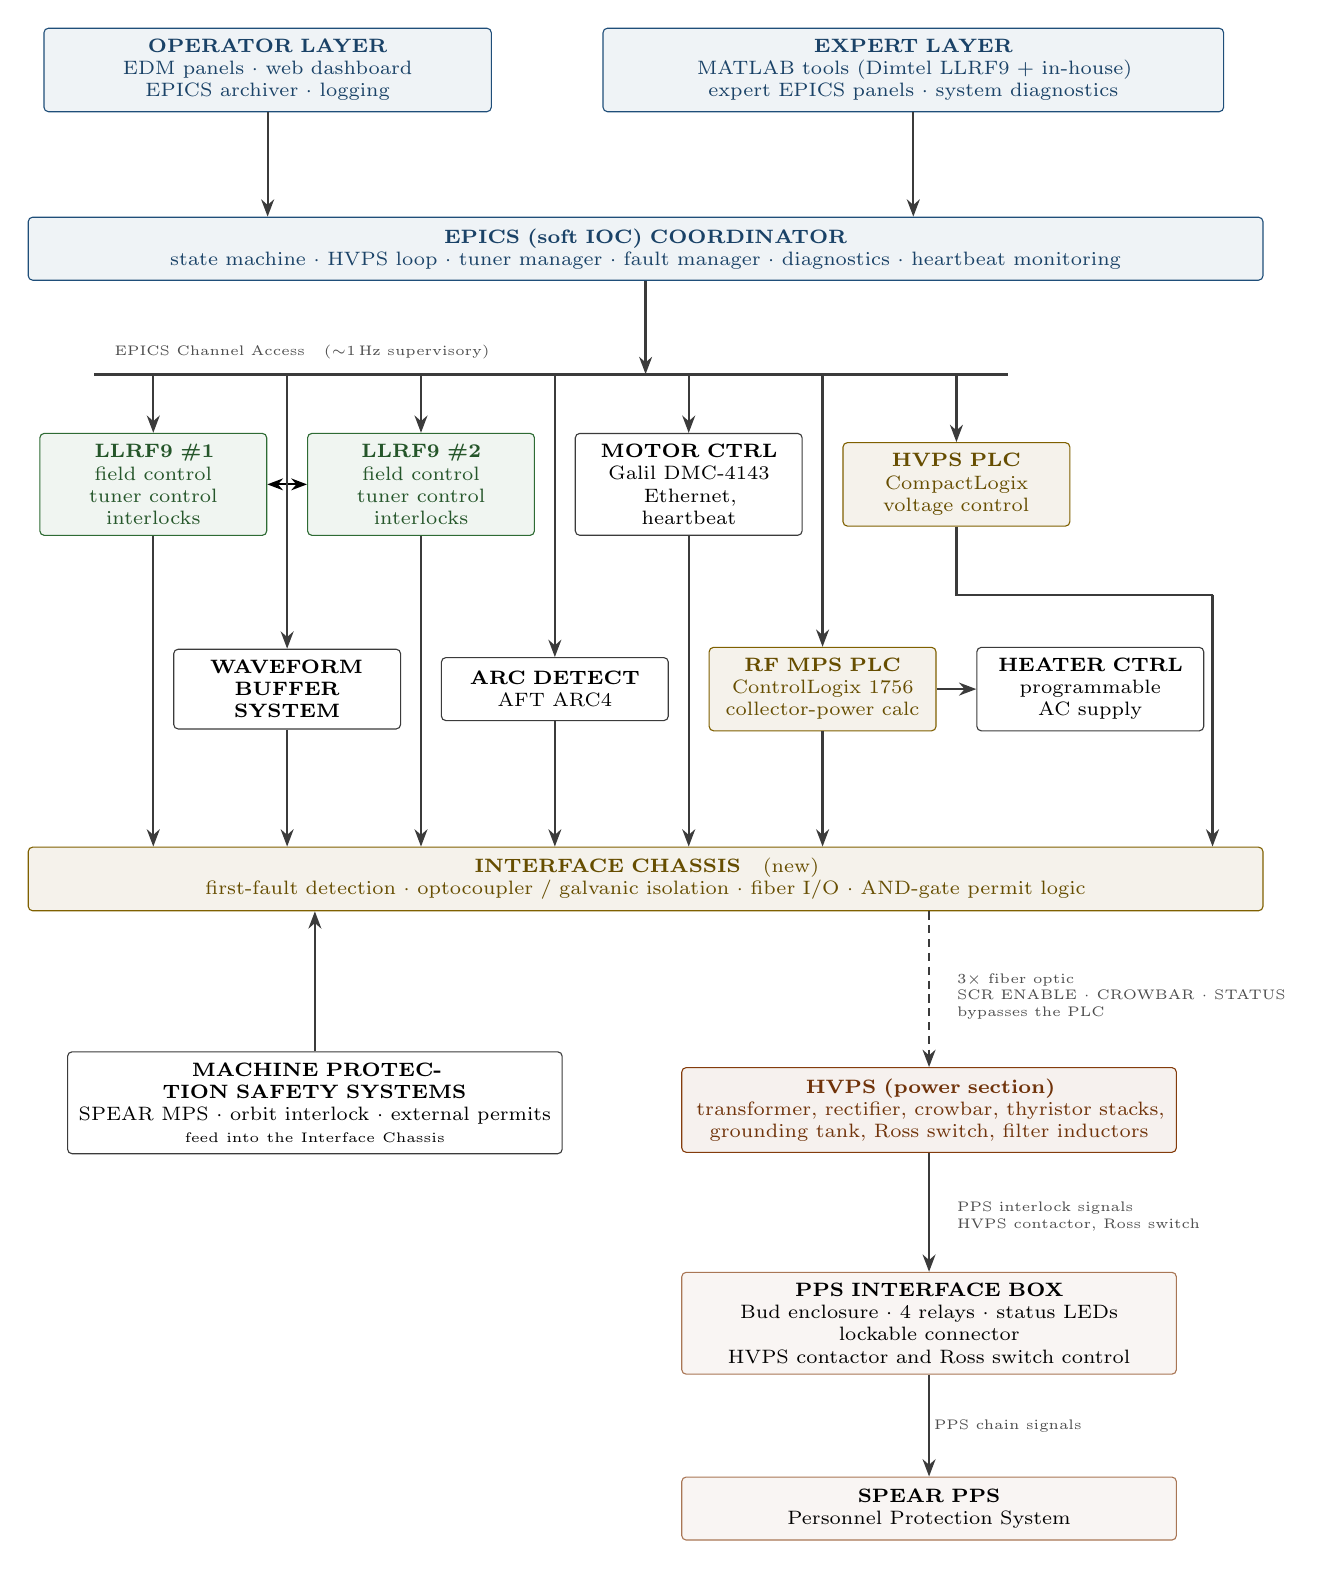
\begin{tikzpicture}[font=\scriptsize, x=1mm, y=1mm]

% ===== operator and expert layers =========================================
\node[ctrl,text width=54mm,anchor=north] (op) at (32,0)
  {\textbf{OPERATOR LAYER}\\
   EDM panels $\cdot$ web dashboard\\ EPICS archiver $\cdot$ logging};
\node[ctrl,text width=76mm,anchor=north] (ex) at (114,0)
  {\textbf{EXPERT LAYER}\\
   MATLAB tools (Dimtel LLRF9 + in-house)\\
   expert EPICS panels $\cdot$ system diagnostics};

% ===== EPICS coordinator ==================================================
\node[ctrl,text width=154mm,anchor=north] (epics) at (80,-24)
  {\textbf{EPICS (soft IOC) COORDINATOR}\\
   state machine $\cdot$ HVPS loop $\cdot$ tuner manager $\cdot$ fault manager
   $\cdot$ diagnostics $\cdot$ heartbeat monitoring};
\draw[sig] (op.south) -- (op.south|-epics.north);
\draw[sig] (ex.south) -- (ex.south|-epics.north);

\def\yCA{-44}
\coordinate (caY) at (0,\yCA);
\draw[bus] (10,\yCA) -- (126,\yCA);
% the rail label sits ABOVE the rail, clear of the coordinator drop at x = 80
\node[tag,anchor=south west,fill=none] at (12,-42.6)
  {EPICS Channel Access\quad($\sim$\qty{1}{\hertz} supervisory)};
\draw[sig] (epics.south) -- (80,\yCA);

% ===== upper subsystem row ================================================
% centres 16 / 50 / 84 / 118, width 26  ->  spans 3-29, 37-63, 71-97, 105-131
\def\yU{-58}
\node[rf,text width=26mm,anchor=west]  (l1)  at (3,\yU)
  {\textbf{LLRF9 \#1}\\ field control\\ tuner control\\ interlocks};
\node[rf,text width=26mm,anchor=west]  (l2)  at (37,\yU)
  {\textbf{LLRF9 \#2}\\ field control\\ tuner control\\ interlocks};
\node[blk,text width=26mm,anchor=west] (mot) at (71,\yU)
  {\textbf{MOTOR CTRL}\\ Galil DMC-4143\\ Ethernet,\\ heartbeat};
\node[plc,text width=26mm,anchor=west] (hp)  at (105,\yU)
  {\textbf{HVPS PLC}\\ CompactLogix\\ voltage control};
\foreach \n in {l1,l2,mot,hp}{\draw[sig] (\n.north|-caY) -- (\n.north);}
% The two LLRF9 interlock chains are wired directly to each other, not via the
% Interface Chassis.  Unlabelled on purpose: the only clear space for a label
% is the lane the Waveform Buffer feed uses.  Explained in the caption.
\draw[{Stealth[length=2mm]}-{Stealth[length=2mm]},thick] (l1.east) -- (l2.west);

% ===== lower subsystem row ================================================
% centres 33 / 67 / 101 / 135, width 26  ->  spans 20-46, 54-80, 88-114, 122-148
\def\yL{-84}
\node[blk,text width=26mm,anchor=west] (wb)   at (20,\yL)
  {\textbf{WAVEFORM}\\\textbf{BUFFER SYSTEM}};
\node[blk,text width=26mm,anchor=west] (arc)  at (54,\yL)
  {\textbf{ARC DETECT}\\ AFT ARC4};
\node[plc,text width=26mm,anchor=west] (mp)   at (88,\yL)
  {\textbf{RF MPS PLC}\\ ControlLogix 1756\\ collector-power calc};
\node[blk,text width=26mm,anchor=west] (heat) at (122,\yL)
  {\textbf{HEATER CTRL}\\ programmable AC supply};
% straight drops: 33, 67 and 101 all fall in gaps of the upper row
\foreach \n in {wb,arc,mp}{\draw[sig] (\n.north|-caY) -- (\n.north);}
\draw[sig] (mp.east) -- (heat.west);

% ===== interface chassis ==================================================
\node[plc,text width=154mm,anchor=north] (ic) at (80,-104)
  {\textbf{INTERFACE CHASSIS}\quad(new)\\
   first-fault detection $\cdot$ optocoupler / galvanic isolation $\cdot$
   fiber I/O $\cdot$ AND-gate permit logic};

% straight drops: 16, 50, 84 all fall in gaps of the lower row
\foreach \n in {l1,l2,mot}{\draw[sig] (\n.south) -- (\n.south|-ic.north);}
\foreach \n in {wb,arc,mp}{\draw[sig] (\n.south) -- (\n.south|-ic.north);}
% HVPS PLC takes the clear lane to the RIGHT of the heater controller
\draw[draw=cNeut,thick] (hp.south) |- (152,-72);
\draw[sig] (152,-72) -- (152,-104);

% ===== external permits ===================================================
\node[blk,text width=60mm,anchor=north] (ext) at (38,-130)
  {\textbf{MACHINE PROTECTION SAFETY SYSTEMS}\\
   SPEAR MPS $\cdot$ orbit interlock $\cdot$ external permits\\
   {\tiny feed into the Interface Chassis}};
\draw[sig] (ext.north) -- (ext.north|-ic.south);

% ===== HVPS power section =================================================
\node[pwr,text width=60mm,anchor=north] (hvps) at (116,-132)
  {\textbf{HVPS (power section)}\\
   transformer, rectifier, crowbar, thyristor stacks,\\
   grounding tank, Ross switch, filter inductors};
% leaves the BOTTOM edge of the Interface Chassis, not its top
\draw[fib] (ic.south -| hvps.north) -- (hvps.north);
\node[tag,anchor=west,align=left] at (119,-123)
  {3$\times$ fiber optic\\ SCR ENABLE $\cdot$ CROWBAR $\cdot$ STATUS\\
   {\tiny bypasses the PLC}};

% ===== PPS chain (separate path) ==========================================
\node[blk,text width=60mm,anchor=north,draw=cPwr!70,fill=cPwr!5] (ppsbox) at (116,-158)
  {\textbf{PPS INTERFACE BOX}\\
   Bud enclosure $\cdot$ 4 relays $\cdot$ status LEDs\\
   lockable connector\\
   HVPS contactor and Ross switch control};
\draw[sig] (hvps.south) -- (hvps.south|-ppsbox.north);
\node[tag,anchor=west,align=left] at (119,-151)
  {PPS interlock signals\\ {\tiny HVPS contactor, Ross switch}};

\node[blk,text width=60mm,anchor=north,draw=cPwr!70,fill=cPwr!5] (pps) at (116,-184)
  {\textbf{SPEAR PPS}\\ Personnel Protection System};
\draw[sig] (ppsbox.south) -- node[right,tag]{PPS chain signals} (pps.north);
\end{tikzpicture}
\end{fitpicture}
\caption{Upgraded system architecture.  The Interface Chassis is the single hub for machine and equipment protection; personnel safety runs on a physically and logically separate path through the PPS Interface Box to the SPEAR PPS.}\label{fig:upgrade-architecture}
\end{figure}
\textbf{Key Architectural Principle}: The Interface Chassis implements \textbf{machine/equipment protection and operational interlocks} (LLRF/HVPS/RF MPS coordination), while personnel safety (PPS) functions are implemented exclusively in a completely separate, dedicated \textbf{PPS Interface Box}. These two safety-related subsystems are architecturally independent:

\begin{itemize}
\tightlist
\item
  \textbf{Operator Layer}: has relative little control with only necessary readbacks.
\item
  \textbf{Expert Layer}: with details used by system experts to control and read data from the system. There will be MATLAB tools, written by Dmitry for the LLRF9 and written in-house for other systems.
\item
  \textbf{HVPS Power section} has three fiber optic cables between Interface Chassis.
\item
  \textbf{Heater Control}: will be controlled by RF MPS system.
\item
  \textbf{Interface Chassis (Machine/Equipment Protection)}: First-fault detection, optocoupler and/or other galvanic isolation, fiber I/O for LLRF9/HVPS/RF MPS/orbit coordination and other machine-protection interlocks
\item
  \textbf{PPS Interface Box (Personnel Safety / PPS)}: Separate Bud enclosure with 4 relays, status LEDs, PPS-lockable connector for HVPS contactor relay and Ross switch control
\end{itemize}

\subsection{What Stays, What Changes, What Is New}\label{what-stays-what-changes-what-is-new}

\noindent\textbf{Retained Physical Hardware} (same equipment):

\begin{itemize}
\tightlist
\item
  Klystron and its RF output
\item
  4 RF cavities and waveguide distribution (circulator, magic-tees, waveguide loads)
\item
  Stepper motors (M093-FC11 or equivalent) and mechanical tuner assemblies
\item
  Linear potentiometers on tuners (position indication)
\item
  HVPS power electronics (transformer, rectifier, oil system, crowbar)
\item
  Vacuum contactor (Ross HQ3) and contactor controller (Ross HCA-1-A)
\item
  Ross grounding switch, Danfysik DC-CT, Pearson CT-110
\item
  Field cabling (Belden 83715 15C \#16 Teflon, Belden 83709 9C \#16 Teflon)
\end{itemize}

\noindent\textbf{Removed / Decommissioned} (retired outright --- no replacement in kind; their functions move into the Interface Chassis):

\begin{itemize}
\tightlist
\item
  \textbf{VXI crate} (Elma 13-slot) and every module in it --- CPU, Clock Module, RFP, IQA $\times$3 and the AIM --- and with it the Allen-Bradley Remote I/O serial link that the Slot 1 scanner mastered
\item
  \textbf{Fast Interlock Chassis 340-308} --- the legacy fast trip-decision element. Its fiber-optic arc inputs, reflected-power comparators and SCR ENABLE / CROWBAR outputs are all absorbed by the Interface Chassis.
\item
  \textbf{AIM --- Arc/Interlock Module} (VXI Slot 12, SLAC drawing 340-307), the digital companion to the Fast IC. Its per-channel arc latching and \texttt{RF\_FAULT} backplane assertion are replaced by the Interface Chassis first-fault register; its fault-history ring buffer is replaced by the Waveform Buffer circular buffers.
\item
  \textbf{Local Panel 340-310} --- legacy local/remote control and indication panel (drawings in \fpath{llrf/documentation/localPanel/}). Local control moves to the Interface Chassis front panel and to EPICS.
\end{itemize}

%\textbf{Note}: the \textbf{Local Control Chassis} --- a separate B132 chassis that aggregated part of the station's hardwired interlock and control wiring and fed the Fast IC --- has no documented I/O list. Whether any of that wiring is re-terminated on the Interface Chassis or retired with the Fast IC is an open item (Section~\ref{open-interface-questions}).

\noindent\textbf{Replaced / Upgraded}:

\begin{itemize}
\tightlist
\item
  LLRF Controller: Analog RFP → Dimtel LLRF9/476 (×2 units)
\item
  RF MPS: PLC-5 1771 → ControlLogix 1756
\item
  HVPS Controller: SLC-500 → CompactLogix PLC + new Enerpro board + redesigned analog regulator
\item
  Tuner Motor Controllers: AB 1746-HSTP1 + Slo-Syn (\textbf{in service}) → Galil DMC-4143 Rev 1.3h 4-axis motion controller (\textbf{in development --- not installed, not operating; goes online when the LLRF upgrade completes}) (commissioned August 2025, operational)

  \begin{itemize}
  \tightlist
  \item
    See: \fpath{llrf/tuners/galil/functioningGalil20250825SwapABToManual.txt}, \fpath{llrf/tuners/galil/firstMotion2024.txt}
  \end{itemize}
\item
  Control Software: SNL/VxWorks → EPICS + LLRF9 internal EPICS IOC + MATLAB applications
\item
  Operator Interface: Legacy EDM panels → modernized panels
\end{itemize}

\noindent\textbf{New Subsystems} (did not exist in legacy):

\begin{itemize}
\tightlist
\item
  Interface Chassis --- central hardware interlock coordination hub
\item
  Waveform Buffer System --- 8 RF + 4 HVPS channel extended monitoring (shares one physical chassis with the Interface Chassis, on a separate PCB)
\item
  Arc Detection --- \textbf{AFT microwave GmbH ARC4} vendor chassis with 12 optical detector modules: 8 cavity window channels (2 per cavity), 1 klystron output window, 1 circulator, 2 spares. Existing tunnel fibers will be test and replaced as needed; no viewport or mechanical adapter work is required.
\item
  PPS Interface Box
\end{itemize}

\noindent\textbf{Enhanced Subsystems} (upgraded from legacy):

\begin{itemize}
\tightlist
\item
  Klystron Heater Controller --- Motor-driven variac → \textbf{TDK Lambda} programmable AC supply with an external \qty{60}{\hertz} sync circuit; MPS controls via analog ramp, EPICS monitors/enables over Ethernet.
\item
  Collector Power Protection --- Forward power proxy → Waveform Buffer System measures HVPS voltage and current and klystron forward power → Collector power calculation performed in RF MPS
\end{itemize}

\begin{center}\rule{0.5\linewidth}{0.5pt}\end{center}

\section{Physical Layout and Locations}\label{physical-layout-and-locations}

The SPEAR3 RF station spans multiple buildings and locations at SSRL:

\begin{longtable}[]{@{}P{\dimexpr 0.2104\linewidth-1.33\tabcolsep\relax}P{\dimexpr 0.6188\linewidth-1.33\tabcolsep\relax}P{\dimexpr 0.1708\linewidth-1.33\tabcolsep\relax}@{}}
\toprule\noalign{}
\begin{minipage}[b]{\linewidth}\raggedright
Location
\end{minipage} & \begin{minipage}[b]{\linewidth}\raggedright
Equipment
\end{minipage} & \begin{minipage}[b]{\linewidth}\raggedright
Notes
\end{minipage} \\
\midrule\noalign{}
\endhead
\bottomrule\noalign{}
\endlastfoot
\textbf{Building B118} (Power Supply Room) & HVPS Controller (Hoffman Box) & HVPS control location \\
\textbf{Building B514} (HVPS Substation) & HVPS Main Tank (transformer, rectifier, inductor, filter caps), Phase Tank (12 thyristor stacks), Crowbar Tank (4 thyristor stacks, output V-divider) & High-voltage power section; FR3 oil-filled, N₂ blanket \\
\textbf{Contactor Disconnect Panel} (Switchgear, B514) & Vacuum contactor (Ross HQ3), Contactor controller (Ross HCA-1-A), K4/MX/RR/L1 relays, S5 auxiliary contact & 12.47 kV AC switchgear \\
\textbf{Termination Tank} (B132, near klystron) & HV cable termination, Ross Engineering HV relay, Danfysik DC-CT, Pearson CT-110 & Mineral oil filled \\
\textbf{Switch-over Tank} (adjacent B514) & HV cable connections between HVPS1/HVPS2 and klystron & FR3 oil filled \\
\textbf{Building B132} (Klystron) & Klystron, drive amplifier, LLRF9 units, RF MPS PLC, combined Interface Chassis / Waveform Buffer chassis, Motion Controller, AFT ARC4 arc detection chassis, soft IOC (may be in B137 --- not yet confirmed with the controls group\openitem{O1}) & Main control electronics location \\
\textbf{SPEAR3 Storage Ring Tunnel} & 4 RF cavities, waveguide distribution, tuner assemblies, arc detection sensors & Radiation area \\
\end{longtable}

\subsection{Cabling Between Locations}\label{cabling-between-locations}

\begin{longtable}[]{@{}P{\dimexpr 0.1794\linewidth-1.50\tabcolsep\relax}P{\dimexpr 0.1421\linewidth-1.50\tabcolsep\relax}P{\dimexpr 0.4228\linewidth-1.50\tabcolsep\relax}P{\dimexpr 0.2556\linewidth-1.50\tabcolsep\relax}@{}}
\toprule\noalign{}
\begin{minipage}[b]{\linewidth}\raggedright
Cable Run
\end{minipage} & \begin{minipage}[b]{\linewidth}\raggedright
Cable Type
\end{minipage} & \begin{minipage}[b]{\linewidth}\raggedright
Conductors
\end{minipage} & \begin{minipage}[b]{\linewidth}\raggedright
Route
\end{minipage} \\
\midrule\noalign{}
\endhead
\bottomrule\noalign{}
\endlastfoot
B118 → Switchgear (Contactor) & Belden 83715 & 15C \#16 Teflon & TS-5 to contactor controller \\
B118 → Termination Tank (Grounding) & Belden 83709 + Belden 83715 & 9C + 15C \#16 Teflon & TS-6 to grounding tank \\
B118 → B514 (HVPS) & Electrical cable pairs & SCR trigger cables (12 pairs) & Controller to Phase Tank thyristor stacks \\
B118 → B514 (HVPS) & Fiber optic & SCR ENABLE, CROWBAR, STATUS & Controller to HVPS (upgrade: via Interface Chassis) \\
B132 → Tunnel & Coax cables & RF signals (forward, reflected, probe). Similar forward, reflected power from klystron and circulator load with B132 & LLRF inputs from cavities \\
B132 → Tunnel & Multi-conductor & Motor power + encoder signals & To tuner assemblies \\
\end{longtable}

\begin{center}\rule{0.5\linewidth}{0.5pt}\end{center}

\section{RF Plant --- Retained Physical Infrastructure}\label{rf-plant-retained-physical-infrastructure}

The RF plant is the physical chain that delivers 476.3 MHz RF power from the klystron to the storage ring beam. All of this hardware is retained as-is during the upgrade.

\subsection{Klystron}\label{klystron}

The single klystron is located in Building B132 and operates at approximately 800 kW output power, driven at \textasciitilde29 W input from the drive amplifier. The klystron cathode is powered by the HVPS at up to \textasciitilde90 kV (nominal \textasciitilde74.7 kV at 500 mA beam current). It has a non-full-power collector requiring dedicated protection (see Section 11.3 for upgrade and current implementation in Section 4.5).

\subsection{Waveguide Distribution}\label{waveguide-distribution}

The klystron output feeds a waveguide network consisting of:

\begin{itemize}
\tightlist
\item
  A circulator (protects klystron from reflected power)
\item
  Magic-tee power splitters (two stage splitter that distributes power to 4 cavities)
\item
  Waveguide loads (absorb rejected power)
\end{itemize}

\subsection{RF Cavities}\label{rf-cavities}

Four single-cell cavities at 476 MHz, each contributing \textasciitilde712 kV gap voltage for a total of \textasciitilde2.85 MV. Each cavity has:

\begin{itemize}
\tightlist
\item
  A cavity probe (monitors internal field amplitude and phase)
\item
  A forward power coupler
\item
  A reflected power coupler
\item
  An individual stepper motor tuner (adjusts resonant frequency via mechanical plunger)
\item
  Waveguide window viewports on either side of a ceramic window (for arc detection sensor mounting)
\end{itemize}

\subsection{Drive Amplifier}\label{drive-amplifier}

The drive amplifier is located in Building B132 near the klystron and boosts the LLRF9 output signal (\textasciitilde0 dBm) to \textasciitilde29 W to drive the klystron input. In the upgrade, the LLRF9 Unit 1 output (from the thermally stabilized output chain on Board 1 or Board 2) connects to the drive amplifier input via coax cable. A KAW2051M12 amplifier datasheet is available in \fpath{llrf/driveAmp/}.

\subsection{Legacy Collector Power Protection}\label{legacy-collector-power-protection}

The current SPEAR3 system includes collector power protection implemented through the HVPS control loop. The legacy system monitors klystron forward power and compares it against configurable limits:

\textbf{Current Implementation}:

\begin{itemize}
\tightlist
\item
  \textbf{Monitoring}: \fpath{LLRF:HVPS:PCOLL_MAX} PV sets maximum collector power limit
\item
  \textbf{Protection Logic}: HVPS loop (\fpath{rf_hvps_loop.st,v}) monitors \fpath{klystron_forward_power} vs.~\fpath{max_klystron_forward_power}
\item
  \textbf{Action}: When klystron forward power exceeds limits, HVPS voltage is reduced (\fpath{delta_proc_voltage_down})
\item
  \textbf{Integration}: Collector limit displayed in HVPS EDL panel (``COLLECTOR LIMIT'')
\end{itemize}

\begin{quote}
\textbf{Note}: In addition to the software protection above, there is an MPS limit (responding on the order of ms) that removes the permit from the HVPS if the limit is exceeded. The fast interlock chassis has an internal RF detector module that takes a coupled signal from the klystron forward power. The AB controller monitors HVPS V and I and performs the arithmetic, removing the MPS permit if collector power exceeds the allowable value. Removal of the permit turns off both the HVPS and the drive power.
\end{quote}

\textbf{Legacy Limitations}:

\begin{itemize}
\tightlist
\item
  No direct DC power measurement
\end{itemize}

\subsection{RF Signal Monitoring}\label{rf-signal-monitoring}

The amplitudes of the RF data need to be acquired. The RF signals that are currently monitored are listed in the table below, along with their location in the RF plant signal flow.

\begin{figure}[tbp]
\centering
\resizebox{0.82\linewidth}{!}{% !TeX root = ../0_system_design_report.tex
% Figure 2 -- RF plant signal flow.  Circled numbers are the directional-coupler
% channel indices (1)-(24) used in the "Monitored RF Signals" table.
% Row members use anchor=west at a common y so every in-row connector is exactly
% horizontal; every branch uses -| so no run is ever diagonal.
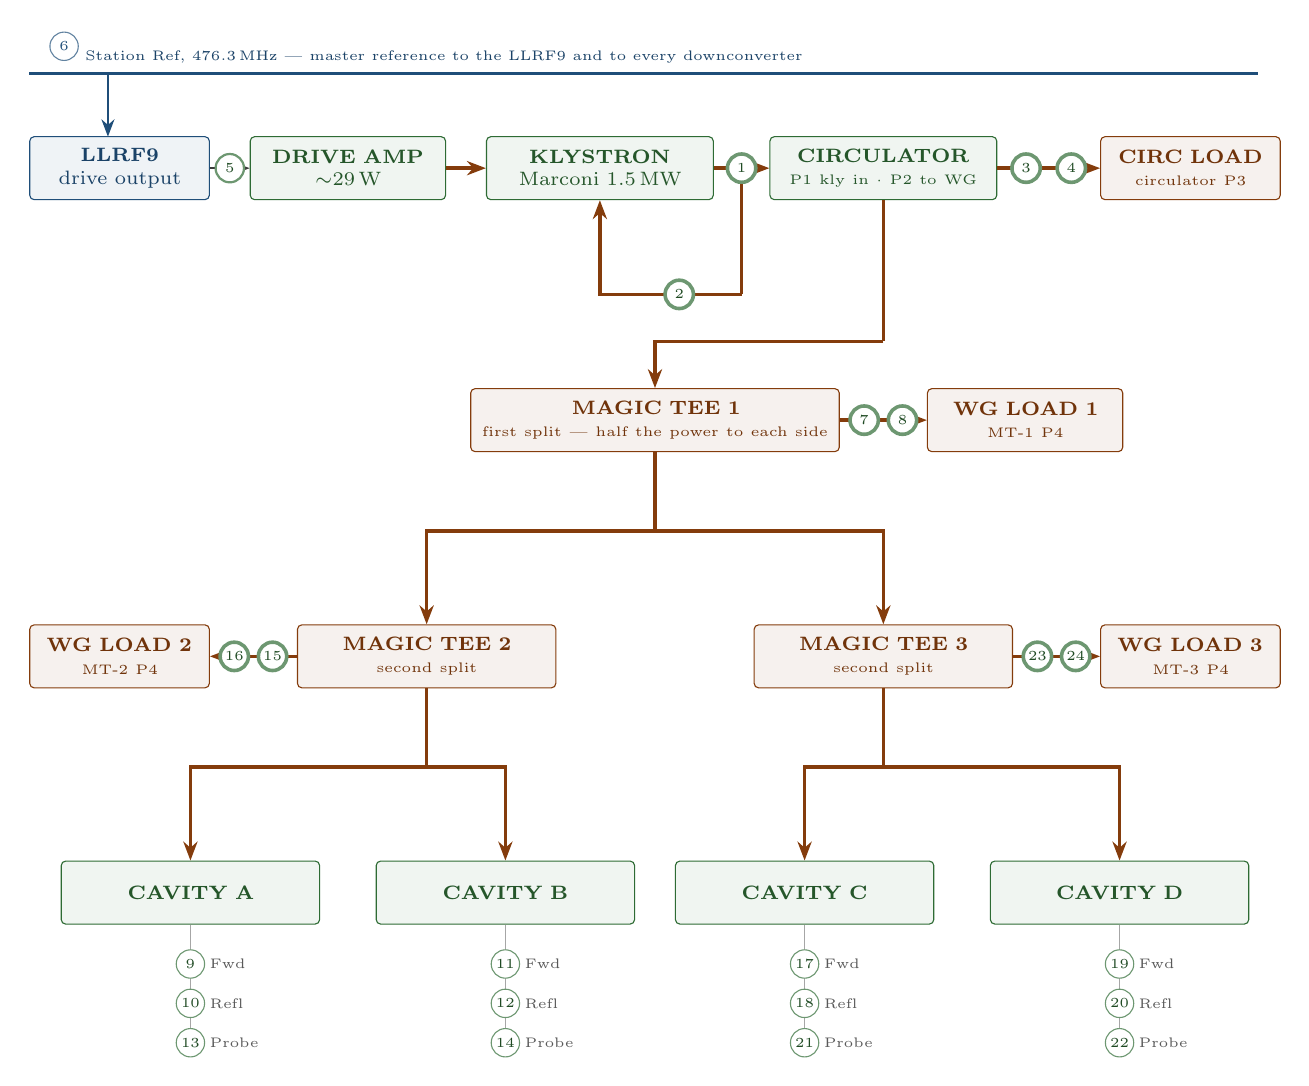
\begin{tikzpicture}[
  font=\scriptsize, x=1mm, y=1mm,
  sn/.style={circle,draw=cRf!70,fill=white,inner sep=0.3pt,font=\tiny,
             text=cRf!70!black,minimum size=3.6mm},
  wg/.style={draw=cPwr,line width=1.3pt,-{Stealth[length=2.4mm]}},
  wgp/.style={draw=cPwr,line width=1.3pt},
]

% ===== station reference rail ============================================
\draw[bus,draw=cCtrl] (0,12) -- (156,12);
\node[tag,anchor=south west,text=cCtrl!85!black] at (2,12.8)
  {\tikz[baseline=-0.6ex]\node[sn,draw=cCtrl!70,text=cCtrl]{6};\ %
   Station Ref, \qty{476.3}{\mega\hertz} --- master reference to the LLRF9 and
   to every downconverter};
\draw[sig,draw=cCtrl] (10,12) -- (10,4);

% ===== drive chain =======================================================
\node[ctrl,text width=20mm,anchor=west] (llrf) at (0,0)  {\textbf{LLRF9}\\ drive output};
\node[rf,text width=22mm,anchor=west]   (amp)  at (28,0) {\textbf{DRIVE AMP}\\ $\sim$\qty{29}{\watt}};
\node[rf,text width=26mm,anchor=west]   (kly)  at (58,0) {\textbf{KLYSTRON}\\ Marconi \qty{1.5}{\mega\watt}};
\node[rf,text width=26mm,anchor=west]   (circ) at (94,0)
  {\textbf{CIRCULATOR}\\ {\tiny P1 kly in $\cdot$ P2 to WG}};
\node[pwr,text width=20mm,anchor=west]  (cl)   at (136,0)
  {\textbf{CIRC LOAD}\\ {\tiny circulator P3}};

\draw[sig] (llrf.east) -- node[sn]{5} (amp.west);
\draw[wg]  (amp.east)  -- (kly.west);
\draw[wg]  (kly.east)  -- node[sn] (n1) {1} (circ.west);
\draw[wg]  (circ.east) -- node[sn,pos=0.28]{3} node[sn,pos=0.72]{4} (cl.west);

% Klystron reflected power.  Same directional coupler as (1), so the branch
% drops out of the BOTTOM of the (1) marker rather than from a bare point on
% the waveguide run.
\coordinate (r2) at ($(n1.south)+(0,-14)$);
\draw[wgp] (n1.south) -- (r2);
\draw[wg]  (r2) -| node[sn,pos=0.22]{2} (kly.south);

% ===== magic tee 1 =======================================================
\node[pwr,text width=44mm,anchor=west] (mt1) at (56,-32)
  {\textbf{MAGIC TEE 1}\\ {\tiny first split --- half the power to each side}};
\node[pwr,text width=22mm,anchor=west] (wl1) at (114,-32)
  {\textbf{WG LOAD 1}\\ {\tiny MT-1 P4}};
\draw[wg] (mt1.east) -- node[sn,pos=0.28]{7} node[sn,pos=0.72]{8} (wl1.west);
% circulator P2 down into MT1
\coordinate (p2) at (107,-22);
\draw[wgp] (circ.south) -- (circ.south|-p2);
\draw[wg]  (circ.south|-p2) -| (mt1.north);

% ===== magic tee 2 / 3 ===================================================
\node[pwr,text width=20mm,anchor=west] (wl2) at (0,-62)
  {\textbf{WG LOAD 2}\\ {\tiny MT-2 P4}};
\node[pwr,text width=30mm,anchor=west] (mt2) at (34,-62)
  {\textbf{MAGIC TEE 2}\\ {\tiny second split}};
\node[pwr,text width=30mm,anchor=west] (mt3) at (92,-62)
  {\textbf{MAGIC TEE 3}\\ {\tiny second split}};
\node[pwr,text width=20mm,anchor=west] (wl3) at (136,-62)
  {\textbf{WG LOAD 3}\\ {\tiny MT-3 P4}};
\draw[wg] (mt2.west) -- node[sn,pos=0.28]{15} node[sn,pos=0.72]{16} (wl2.east);
\draw[wg] (mt3.east) -- node[sn,pos=0.28]{23} node[sn,pos=0.72]{24} (wl3.west);

\coordinate (s1) at ($(mt1.south)+(0,-10)$);
\draw[wgp] (mt1.south) -- (s1);
\draw[wg]  (s1) -| (mt2.north);
\draw[wg]  (s1) -| (mt3.north);

% ===== cavities ==========================================================
\def\yC{-92}
\node[rf,text width=30mm,anchor=west] (ca) at (4,\yC)   {\textbf{CAVITY A}};
\node[rf,text width=30mm,anchor=west] (cb) at (44,\yC)  {\textbf{CAVITY B}};
\node[rf,text width=30mm,anchor=west] (cc) at (82,\yC)  {\textbf{CAVITY C}};
\node[rf,text width=30mm,anchor=west] (cd) at (122,\yC) {\textbf{CAVITY D}};

\coordinate (s2) at ($(mt2.south)+(0,-10)$);
\draw[wgp] (mt2.south) -- (s2);
\draw[wg]  (s2) -| (ca.north);
\draw[wg]  (s2) -| (cb.north);
\coordinate (s3) at ($(mt3.south)+(0,-10)$);
\draw[wgp] (mt3.south) -- (s3);
\draw[wg]  (s3) -| (cc.north);
\draw[wg]  (s3) -| (cd.north);

% Per-cavity directional-coupler channels.  Each cavity drops a thin spine and
% the three numbered taps hang off it, so all four groups align exactly.
\newcommand{\cavsig}[4]{%
  \draw[draw=black!35] (#1.south) -- ($(#1.south)+(0,-15)$);
  \node[sn] (#1a) at ($(#1.south)+(0,-5)$)  {#2};
  \node[sn] (#1b) at ($(#1.south)+(0,-10)$) {#3};
  \node[sn] (#1c) at ($(#1.south)+(0,-15)$) {#4};
  \node[anchor=west,font=\tiny,text=black!65,inner sep=1.5pt] at (#1a.east) {Fwd};
  \node[anchor=west,font=\tiny,text=black!65,inner sep=1.5pt] at (#1b.east) {Refl};
  \node[anchor=west,font=\tiny,text=black!65,inner sep=1.5pt] at (#1c.east) {Probe};}
\cavsig{ca}{9}{10}{13}
\cavsig{cb}{11}{12}{14}
\cavsig{cc}{17}{18}{21}
\cavsig{cd}{19}{20}{22}
\end{tikzpicture}
}
\caption{RF plant signal flow.  Heavy lines are waveguide, light lines coaxial.  Circled numbers are the directional-coupler channel indices used in \Cref{rf-signal-monitoring}.  Channel~2 (klystron reflected power) branches from the bottom of channel~1 because both are ports of the same directional coupler between the klystron and the circulator.}\label{fig:rf-signal-flow}
\end{figure}
\subsubsection{Monitored RF Signals}\label{monitored-rf-signals}

\begin{longtable}[]{@{}P{\dimexpr 0.0428\linewidth-1.50\tabcolsep\relax}P{\dimexpr 0.1256\linewidth-1.50\tabcolsep\relax}P{\dimexpr 0.1035\linewidth-1.50\tabcolsep\relax}P{\dimexpr 0.7281\linewidth-1.50\tabcolsep\relax}@{}}
\toprule\noalign{}
\begin{minipage}[b]{\linewidth}\raggedright
\#
\end{minipage} & \begin{minipage}[b]{\linewidth}\raggedright
Signal
\end{minipage} & \begin{minipage}[b]{\linewidth}\raggedright
Monitored By
\end{minipage} & \begin{minipage}[b]{\linewidth}\raggedright
Notes
\end{minipage} \\
\midrule\noalign{}
\endhead
\bottomrule\noalign{}
\endlastfoot
1 & Klystron Output Forward Power & LLRF9 Unit 2 BRD2 & RF power at the klystron output traveling toward the circulator; primary measure of station RF output level. \\
2 & Klystron Output Reflected Power & LLRF9 Unit 2 BRD2 & RF power reflected back into the klystron output port from the load chain; should be near zero; used for klystron protection. \\
3 & Circulator Load Forward Power & LLRF9 Unit 1 BRD3 & Power delivered to the circulator load (circulator port 3); absorbs power the circulator does not properly direct to the cavities plus any net reflection returning from the waveguide network. Sits at \textasciitilde20 kW, increases to \textasciitilde40 kW at full power with no beam --- more significant signal than WG Load 1 Fwd. \\
4 & Circulator Load Reflected Power & Waveform Buffer Ch2 & Power reflected from the circulator load back into the circulator; indicates load match quality. \\
5 & Klystron Drive Power & LLRF9 Unit 2 BRD1 & Input drive signal level to the klystron from the drive amplifier; sets the klystron gain and operating point. \\
6 & Station Reference Power & Waveform Buffer Ch3 & Monitor of the 476 MHz reference signal level distributed to the LLRF system; loss of this signal indicates a reference chain fault. \\
7 & Waveguide Load 1 Forward Power & Waveform Buffer (slow) & Power entering WG Load 1 at port 4 of Magic Tee 1. Rarely exceeds 2 kW --- suitable for slow monitoring only. \\
8 & Waveguide Load 1 Reflected Power & Waveform Buffer Ch4 & Power reflected from WG Load 1 back into Magic Tee 1; indicates load match quality. \\
9 & Cavity A Forward Power & LLRF9 Unit 1 BRD1 & RF power traveling into Cavity A from Magic Tee 2; used to monitor power distribution balance and provide reference phase for cavity probe phase measurement. \\
10 & Cavity A Reflected Power & LLRF9 Unit 2 BRD3 & Power reflected from Cavity A back into the waveguide; elevated reflection indicates cavity detuning or mismatch. \\
11 & Cavity B Forward Power & LLRF9 Unit 1 BRD2 & RF power traveling into Cavity B from Magic Tee 2; compared with Cavity A forward to verify magic-tee balance and provide reference phase for cavity probe phase measurement. \\
12 & Cavity B Reflected Power & LLRF9 Unit 2 BRD3 & Power reflected from Cavity B; monitored for detuning and arc detection. \\
13 & Cavity A Probe Signal & LLRF9 Unit 1 BRD1 & Electric field sampled by Cavity A's internal pickup probe; direct measure of the accelerating voltage amplitude and phase; primary LLRF fast feedback and tuner control input for Cavity A. \\
14 & Cavity B Probe Signal & LLRF9 Unit 1 BRD1 & Electric field from Cavity B's internal probe; used in the LLRF vector-sum feedback and Cavity B tuner control. \\
15 & Waveguide Load 2 Forward Power & LLRF9 Unit 1 BRD3 & Power entering WG Load 2 at port 4 of Magic Tee 2; absorbs the sum of equal reflected power from Cavities A and B. \\
16 & Waveguide Load 2 Reflected Power & Waveform Buffer Ch5 & Power reflected from WG Load 2; indicates match quality of the load. \\
17 & Cavity C Forward Power & LLRF9 Unit 1 BRD2 & RF power traveling into Cavity C from Magic Tee 3. \\
18 & Cavity C Reflected Power & LLRF9 Unit 2 BRD3 & Power reflected from Cavity C; monitored for detuning and arc detection. \\
19 & Cavity D Forward Power & LLRF9 Unit 2 BRD1 & RF power traveling into Cavity D from Magic Tee 3. \\
20 & Cavity D Reflected Power & LLRF9 Unit 2 BRD2 & Power reflected from Cavity D. \\
21 & Cavity C Probe Signal & LLRF9 Unit 1 BRD2 & Electric field from Cavity C's internal probe; used in the LLRF vector-sum feedback and Cavity C tuner control. \\
22 & Cavity D Probe Signal & LLRF9 Unit 2 BRD1 & Electric field from Cavity D's internal probe; used in the LLRF vector-sum feedback and Cavity D tuner control. \\
23 & Waveguide Load 3 Forward Power & LLRF9 Unit 1 BRD3 & Power entering WG Load 3 at port 4 of Magic Tee 3; absorbs the sum of equal reflected power from Cavities C and D. \\
24 & Waveguide Load 3 Reflected Power & Waveform Buffer Ch6 & Power reflected from WG Load 3; indicates match quality of the load. \\
\end{longtable}

\begin{center}\rule{0.5\linewidth}{0.5pt}\end{center}

\section{Subsystem 1: LLRF Controller}\label{subsystem-1-llrf-controller}

\begin{quote}
\textbf{Detailed reference}: \texttt{llrf/llrf9}
\end{quote}

\subsection{Legacy System}\label{legacy-system}

The legacy LLRF controller is a custom PEP-II analog RF Processor (RFP) module in a VXI chassis. It performs analog I/Q processing at \textasciitilde+/-90 kHz bandwidth for the fast RF feedback loop. Associated modules include the Clock Module and three IQA (\textasciitilde1 MHz amplitude and phase detector) modules. The VXI chassis also hosts a processor running VxWorks RTOS with SNL (State Notation Language) control programs.

The legacy system processes 24 RF channels through the VXI system and uses analog-domain signal processing for feedback and calibration.

\subsection{Upgraded System --- Dimtel LLRF9/476}\label{upgraded-system-dimtel-llrf9476}

Two Dimtel LLRF9/476 units replace the entire VXI-based LLRF system (four units purchased; two active, two spares).

\textbf{Hardware per unit}:

\begin{itemize}
\tightlist
\item
  3 × LLRF4.6 boards: each with a Xilinx FPGA, 4 high-speed ADC channels, 2 DAC channels, 3 RF channels
\item
  LO/Interconnect module: divide-and-mix LO synthesis for low phase noise, RF reference distribution, output amplification/filtering, interlock logic
\item
  Linux SBC (mini-ITX): runs the built-in EPICS IOC. Dmitry upgraded it from EPICS Base 3.14 to EPICS 7 in June 2026, so it now matches the SSRL site standard.
\item
  Thermal stabilization: aluminum cold plate with 3 TEC modules under PID control, only available to board1\&2
\item
  Power supply: 90-264 VAC auto-ranging
\item
  3U 19'' rack chassis
\end{itemize}

\textbf{LO Frequency Plan (LLRF9/476)} --- nominal frequency 476.3 MHz (current: 476.3051755 MHz):

\begin{longtable}[]{@{}P{\dimexpr 0.3502\linewidth-1.33\tabcolsep\relax}P{\dimexpr 0.2296\linewidth-1.33\tabcolsep\relax}P{\dimexpr 0.4202\linewidth-1.33\tabcolsep\relax}@{}}
\toprule\noalign{}
Signal & Ratio to f\_rf & Nominal Frequency (MHz) \\
\midrule\noalign{}
\endhead
\bottomrule\noalign{}
\endlastfoot
Reference (f\_rf) & 1 & 476.3052 \\
IF & 1/12 & 39.6921 \\
Local Oscillator & 11/12 & 436.6131 \\
ADC Clock & 11/48 & 109.1533 \\
DAC Clock & 11/24 & 218.3065 \\
\end{longtable}

\textbf{Auxiliary I/O per unit}:

\begin{itemize}
\tightlist
\item
  8 slow ADC channels (12-bit, selectable ranges, galvanically isolated)
\item
  12 slow DAC outputs (AD5644)
\item
  Opto-isolated interlock input (3.3V/5V/24V selectable --- confirm exact voltage logic levels from test summaries)
\item
  Interlock output (+4.75V high / \textless0.1V tripped, 220 Ω)
\item
  Two opto-isolated trigger inputs
\end{itemize}

\subsection{Two-Unit Configuration for SPEAR3}\label{two-unit-configuration-for-spear3}

\textbf{Unit 1 --- Field Control \& Tuner Loops}:

\begin{longtable}[]{@{}P{\dimexpr 0.0781\linewidth-1.71\tabcolsep\relax}P{\dimexpr 0.1554\linewidth-1.71\tabcolsep\relax}P{\dimexpr 0.1486\linewidth-1.71\tabcolsep\relax}P{\dimexpr 0.1435\linewidth-1.71\tabcolsep\relax}P{\dimexpr 0.1384\linewidth-1.71\tabcolsep\relax}P{\dimexpr 0.1852\linewidth-1.71\tabcolsep\relax}P{\dimexpr 0.1507\linewidth-1.71\tabcolsep\relax}@{}}
\toprule\noalign{}
\begin{minipage}[b]{\linewidth}\raggedright
Board
\end{minipage} & \begin{minipage}[b]{\linewidth}\raggedright
Ch0 (Ref)
\end{minipage} & \begin{minipage}[b]{\linewidth}\raggedright
Ch1
\end{minipage} & \begin{minipage}[b]{\linewidth}\raggedright
Ch2
\end{minipage} & \begin{minipage}[b]{\linewidth}\raggedright
Ch3
\end{minipage} & \begin{minipage}[b]{\linewidth}\raggedright
Output
\end{minipage} & \begin{minipage}[b]{\linewidth}\raggedright
Thermal Stabilization
\end{minipage} \\
\midrule\noalign{}
\endhead
\bottomrule\noalign{}
\endlastfoot
BRD1 & Station Ref & Cav A Probe & Cav B Probe & Cav A Fwd & Klystron Drive & Y \\
BRD2 & Station Ref & Cav C Probe & Cav C Fwd & Cav B Fwd & (Spare / Monitor) & Y \\
BRD3 & Station Ref & Circ Load Fwd & WG Load 2 Fwd & WG Load 3 Fwd & (Not used) & N \\
\end{longtable}

\begin{itemize}
\tightlist
\item
  \textbf{Feedback Architecture}: Cavity probes A and B can be monitored on BRD1 with proportional and integral control driving output 1. Probes C and D can be monitored on BRD2 with integral control driving output 2. An external power combiner combines the outputs to generate a signal containing an integral of all four cavities. The outputs of the two boards are synchronized via phase controls.
\item
  \textbf{Tuner phase data}: All 4 cavity probe phases available at 10 Hz for tuner control
\end{itemize}

\textbf{Unit 2 --- Monitoring \& Interlocks}:

\begin{longtable}[]{@{}P{\dimexpr 0.0891\linewidth-1.71\tabcolsep\relax}P{\dimexpr 0.1772\linewidth-1.71\tabcolsep\relax}P{\dimexpr 0.1500\linewidth-1.71\tabcolsep\relax}P{\dimexpr 0.1346\linewidth-1.71\tabcolsep\relax}P{\dimexpr 0.1258\linewidth-1.71\tabcolsep\relax}P{\dimexpr 0.1520\linewidth-1.71\tabcolsep\relax}P{\dimexpr 0.1713\linewidth-1.71\tabcolsep\relax}@{}}
\toprule\noalign{}
\begin{minipage}[b]{\linewidth}\raggedright
Board
\end{minipage} & \begin{minipage}[b]{\linewidth}\raggedright
Ch0 (Ref)
\end{minipage} & \begin{minipage}[b]{\linewidth}\raggedright
Ch1
\end{minipage} & \begin{minipage}[b]{\linewidth}\raggedright
Ch2
\end{minipage} & \begin{minipage}[b]{\linewidth}\raggedright
Ch3
\end{minipage} & \begin{minipage}[b]{\linewidth}\raggedright
Output
\end{minipage} & \begin{minipage}[b]{\linewidth}\raggedright
Thermal Stabilization
\end{minipage} \\
\midrule\noalign{}
\endhead
\bottomrule\noalign{}
\endlastfoot
BRD1 & Station Ref & Cav D Probe & Cav D Fwd & Drv Fwd & (Not used) & Y \\
BRD2 & Station Ref & Cav D Refl & Kly Refl & Kly Fwd & (Not used) & Y \\
BRD3 & Station Ref & Cav A Refl & Cav B Refl & Cav C Refl & (Not used) & N \\
\end{longtable}

\begin{itemize}
\tightlist
\item
  \textbf{Reflected power monitoring}: All 4 cavity reflected + klystron reflected for arc/mismatch detection
\item
  \textbf{Interlock chain}: Reflected power events → Unit 2 interlock output → Interface Chassis → disables Unit 1 drive
\item
  \textbf{No drive output required} from Unit 2
\end{itemize}

\begin{quote}
\textbf{Remaining RF signals}: The 6 signals not covered by the two LLRF9 units (Waveguide 1 Load Fwd, Circulator Load Refl, Station Reference, WG Load 1/2/3 Reflected) are monitored by the Waveform Buffer System --- see Section 11.
\end{quote}

\subsection{Key Performance Specifications}\label{key-performance-specifications}

\begin{longtable}[]{@{}P{\dimexpr 0.6272\linewidth-1.00\tabcolsep\relax}P{\dimexpr 0.3728\linewidth-1.00\tabcolsep\relax}@{}}
\toprule\noalign{}
Parameter & Value \\
\midrule\noalign{}
\endhead
\bottomrule\noalign{}
\endlastfoot
Direct loop delay & 270 ns \\
RF input channels & 9 per unit (18 total) \\
RF input range & +2 dBm full-scale \\
ADC resolution & 12-bit \\
Setpoint profile points & 512 \\
Setpoint step time range & 70 μs to 37 ms per step \\
Waveform samples/channel & 16,384 \\
Scalar readback rate & 10 Hz \\
Phase readback resolution & Sub-degree \\
Interlock timestamp resolution & $\pm$17.4 ns \\
\end{longtable}

\subsection{Interfaces}\label{interfaces}

\begin{itemize}
\tightlist
\item
  \textbf{RF inputs}: 50 Ω SMA from cavity probes, forward couplers, reflected couplers, station reference
\item
  \textbf{RF output}: SMA to drive amplifier (Unit 1 only, thermally stabilized, BRD1 or BRD2)
\item
  \textbf{Interlock I/O}: LEMO connectors; Unit 1 external interlock input from Interface Chassis, Unit 2 interlock output to Interface Chassis (exact voltage logic levels still to be confirmed from the LLRF9 test summaries\openitem{O2})
\item
  \textbf{Slow ADC}: DA-15 connector; HVPS monitoring signals, auxiliary sensors
\item
  \textbf{Ethernet}: Channel Access for EPICS communication (default ports 5064/5065)
\item
  \textbf{Unit 1 ↔ Unit 2}: Interlock daisy-chain (e.g.~Unit 2 reflected power trip disables Unit 1 drive)
\end{itemize}

\begin{center}\rule{0.5\linewidth}{0.5pt}\end{center}

\section{Subsystem 2: High Voltage Power Supply (HVPS)}\label{subsystem-2-high-voltage-power-supply-hvps}

\begin{quote}
\textbf{Primary source references}: Architecture: \fpath{hvps/architecture/}
\end{quote}

\subsection{Power Section (Retained)}\label{power-section-retained}

Based on the proven PEP-II design architecture from 1997, this legacy system has been adapted for SPEAR3 operational requirements while maintaining the innovative star point controller topology and multi-layer arc protection system. The HVPS converts 12.47 kV RMS 3-phase AC to regulated DC high voltage for the klystron cathode. It is \textbf{rated −90 kV at 27 A (2.5 MW)} and typically operates at \textbf{≈ −72 to −75 kV at 19--22 A (≈ 1.4--1.6 MW DC)}, which supports the klystron's ≈ 800 kW typical RF output. The power section, including transformers, thyristor stacks, filter inductors, secondary rectifiers, crowbar, oil system, and all power cabling, is retained unchanged.

\begin{figure}[p]
\centering
\begin{fitpicture}% !TeX root = ../0_system_design_report.tex
% Figure 3 -- HVPS power chain, B514.  12-pulse phase-controlled rectifier.
%
% Full conversion chain from the incoming substation feeder to the klystron
% cathode.  Component values are the VERIFIED as-built ones from Doc L §9.3 --
% they deliberately differ from the 1997 PEP-II design figures that circulated
% earlier (T0 2750 kVA not 350 kVA; capacitors 8 uF per stage x 4 stages not
% 8 uF total; divider ~10,000:1 not 1000:1; termination inductors 350 uH not
% 200 uH; crowbar conduction ~10 us not ~1 us).
%
% Layout: power chain in a 150 mm column on the right; the Waveform Buffer on
% the left with four dashed monitoring taps.  Tap lanes are ordered so that the
% tap entering the buffer highest uses the leftmost lane -- each horizontal turn
% then passes only over lanes that have already turned, so no tap crosses
% another.  The single deliberate crossing is the Inductor 2 tap over the L1
% power drop; no route avoids it, and dashed blue over solid dark reads clearly.
\begin{tikzpicture}[font=\scriptsize, x=1mm, y=1mm,
  full/.style={pwr,text width=150mm,anchor=north},
  half/.style={pwr,text width=54mm,anchor=north},
  tap/.style ={draw=cCtrl!75,densely dashed,line width=0.6pt,
               -{Stealth[length=1.8mm]}},
  cn/.style  ={circle,draw=cCtrl!70,fill=white,inner sep=0.3pt,font=\tiny,
               text=cCtrl!80!black,minimum size=3.6mm},
]

\node[lbl,anchor=north] at (133,9) {BUILDING B514 --- high-voltage power section};

% ===== incoming feeder ===================================================
\node[full,fill=black!8,draw=black!55,text=black!75] (sub) at (133,0)
  {\textbf{SUBSTATION 507, BREAKER 160}\\
   \qty{12.47}{\kilo\volt} RMS 3-phase AC};

\node[full] (sw) at (133,-16)
  {\textbf{SWITCHGEAR \& SAFETY}\\
   disconnect switch $\cdot$ fuses (3\,$\times$\,\qty{50}{\ampere}) $\cdot$
   vacuum contactor (Ross HQ3)\\
   ground switch $\cdot$ interlocks};
\draw[sig] (sub.south) -- (sw.north);

\node[full] (t0) at (133,-38)
  {\textbf{PHASE-SHIFT TRANSFORMER T0}\\
   extended delta $\cdot$ \qty{2750}{\kilo\voltampere},
   \qty{12.5}{\kilo\volt} at \qty{127}{\ampere} RMS\\
   primary \qty{12.47}{\kilo\volt} delta \quad$\vert$\quad
   secondary dual wye, $\pm 15^\circ$ phase shift};
\draw[sig] (sw.south) -- node[right,tag]{\qty{12.47}{\kilo\volt} delta} (t0.north);

% ===== two rectifier transformers ========================================
\node[half] (t1) at (85,-62)
  {\textbf{RECTIFIER XFMR T1}\\
   \qty{1.5}{\mega\voltampere} $\cdot$ $+15^\circ$\\
   open wye primary $\cdot$ dual wye \qty{12.5}{\kilo\volt}};
\node[half] (t2) at (181,-62)
  {\textbf{RECTIFIER XFMR T2}\\
   \qty{1.5}{\mega\voltampere} $\cdot$ $-15^\circ$\\
   open wye primary $\cdot$ dual wye \qty{12.5}{\kilo\volt}};
\draw[sig] (t1.north|-t0.south) -- node[right,tag]{$+15^\circ$} (t1.north);
\draw[sig] (t2.north|-t0.south) -- node[right,tag]{$-15^\circ$} (t2.north);

% ===== the two 6-pulse bridges, gated from the Interface Chassis =========
\node[half] (b1) at (85,-88)
  {\textbf{6-PULSE BRIDGE B+} (SCR 1--6)\\
   6 stacks $\times$ 14 Powerex T8K7\\ star-point controller};
\node[half] (b2) at (181,-88)
  {\textbf{6-PULSE BRIDGE B$-$} (SCR 7--12)\\
   6 stacks $\times$ 14 Powerex T8K7\\ star-point controller};
\draw[sig] (t1.south) -- (b1.north);
\draw[sig] (t2.south) -- (b2.north);

\node[plc,text width=26mm,anchor=north,draw=cPlc,dashed,align=center] (icx) at (133,-88)
  {\textbf{INTERFACE}\\\textbf{CHASSIS}\\[1pt]
   {\tiny SCR ENABLE\\ CROWBAR}};
\draw[{Stealth[length=2mm]}-,draw=cPlc,thick] (icx.west -| b1.east) -- (icx.west);
\draw[{Stealth[length=2mm]}-,draw=cPlc,thick] (icx.east -| b2.west) -- (icx.east);

% ===== filter inductors ==================================================
\node[half] (l1) at (85,-116)
  {\textbf{FILTER INDUCTOR L1}\\
   \qty{0.3}{\henry} $\cdot$ \qty{85}{\ampere} $\cdot$ \qty{0.38}{\ohm} DC\\
   \qty{1084}{\joule} stored $\cdot$ temp.\ monitored};
\node[half] (l2) at (181,-116)
  {\textbf{FILTER INDUCTOR L2}\\
   \qty{0.3}{\henry} $\cdot$ \qty{85}{\ampere} $\cdot$ \qty{0.38}{\ohm} DC\\
   \qty{1084}{\joule} stored $\cdot$ temp.\ monitored};
\draw[sig] (b1.south) -- (l1.north);
\draw[sig] (b2.south) -- (l2.north);

% the two legs recombine into the series rectifier stack
\draw[draw=cNeut,thick] (l1.south) -- (85,-138) -- (181,-138);
\draw[draw=cNeut,thick] (l2.south) -- (181,-138);

\node[full] (sr) at (133,-144)
  {\textbf{SECONDARY RECTIFIERS D1--D24}\\
   4 six-pulse main bridges in series --- \qty{30}{\kilo\volt},
   \qty{30}{\ampere} each\\
   plus 4 filter bridges --- \qty{30}{\kilo\volt}, \qty{3}{\ampere} average};
\draw[sig] (133,-138) -- (sr.north);

\node[full] (fb) at (133,-166)
  {\textbf{FILTER BANK \& ISOLATION RESISTORS}\\
   capacitors \qty{8}{\micro\farad} per stage $\times$ 4 series stages
   ($\approx$\,\qty{2}{\micro\farad} net, \qty{8.8}{\kilo\joule})\\
   \qty{500}{\ohm} / \qty{1}{\kilo\watt} isolation resistors (PEP-II)
   $\cdot$ output divider $\approx$ 10\,000:1};
\draw[sig] (sr.south) -- (fb.north);

\node[full] (cb) at (133,-188)
  {\textbf{CROWBAR PROTECTION} (SCR 13--16)\\
   4 thyristor stacks in series, \qty{100}{\kilo\volt}\\
   fiber-optic trigger, $\approx$\,\qty{10}{\micro\second} conduction delay
   $\cdot$ dV/dt snubbers\\
   crowbar tank, FR3 oil-filled};
\draw[sig] (fb.south) -- (cb.north);

\node[full] (ti) at (133,-214)
  {\textbf{CABLE TERMINATION INDUCTORS}\\
   \qty{350}{\micro\henry}, \qty{40}{\ampere} each (as built)\\
   limit cable discharge current into the klystron};
\draw[sig] (cb.south) -- (ti.north);

\node[full,fill=cPwr!16,draw=cPwr] (out) at (133,-236)
  {\textbf{KLYSTRON CATHODE} --- \qty{-74}{\kilo\volt} DC at
   \qty{22}{\ampere} typical\\
   {\tiny rated \qty{-90}{\kilo\volt} / \qty{27}{\ampere};
    cable run to Building B132}};
\draw[sig] (ti.south) -- (out.north);

% ===== waveform buffer and its four monitoring taps ======================
% wb spans x = 1..35; entries on its east edge at -163 / -168 / -172 / -178.
\node[ctrl,text width=34mm,anchor=north,align=center] (wb) at (18,-160)
  {\textbf{WAVEFORM}\\\textbf{BUFFER SYSTEM}\\[1pt]
   {\tiny 4 HVPS channels, circular\\ buffers, pre-fault capture}\\[2pt]
   {\tiny \textbf{1} HVPS voltage\\ \textbf{2} HVPS current\\
          \textbf{3} Inductor 1 voltage\\ \textbf{4} Inductor 2 voltage}};

% ch 3 -- Inductor 1 voltage: lane 40, turns first (highest entry)
\draw[tap] (l1.west) -| (40,-163) -- (35,-163);
\node[cn] at (52,-122) {3};

% ch 4 -- Inductor 2 voltage: lane 45.  Crosses the L1 power drop at x = 85.
\draw[tap] (l2.west) -| (150,-133) -- (45,-133) -- (45,-168) -- (35,-168);
\node[cn] at (148,-122) {4};

% ch 1 -- HVPS voltage from the output divider: straight in, no lane needed
\draw[tap] (fb.west) -- (35,-172);
\node[cn] at (52,-172) {1};

% ch 2 -- HVPS current from the output run: lane 50, turns last (lowest entry)
\draw[tap] (out.west) -| (50,-178) -- (35,-178);
\node[cn] at (54,-240.5) {2};
\end{tikzpicture}
\end{fitpicture}
\caption{HVPS power chain in Building B514, from the incoming substation feeder to the klystron cathode.  The \ang{15} phase offset between the two rectifier transformers is what turns two 6-pulse bridges into a single 12-pulse supply.  Dashed blue lines are the four Waveform Buffer monitoring taps, numbered as in \Cref{channel-configuration}; they are the only non-power signals shown.  Component values are the as-built ones verified against the original drawings --- T0 is \qty{2750}{\kilo\voltampere}, the filter capacitors are \qty{8}{\micro\farad} \emph{per stage} across four series stages, the output divider is $\approx$\,10\,000:1, and the cable termination inductors are \qty{350}{\micro\henry}.}\label{fig:hvps-power-chain}
\end{figure}
\begin{longtable}[]{@{}P{\dimexpr 0.4346\linewidth-1.00\tabcolsep\relax}P{\dimexpr 0.5654\linewidth-1.00\tabcolsep\relax}@{}}
\toprule\noalign{}
\begin{minipage}[b]{\linewidth}\raggedright
Parameter
\end{minipage} & \begin{minipage}[b]{\linewidth}\raggedright
Value
\end{minipage} \\
\midrule\noalign{}
\endhead
\bottomrule\noalign{}
\endlastfoot
Maximum output voltage & −90 kV DC \\
Maximum output current & 27 A \\
Maximum output power & 2.5 MW \\
Nominal operating voltage & −74.4 kV \\
Nominal operating current & 22.0 A \\
Nominal operating beam current & 500 mA \\
Rectifier topology & 12-pulse, thyristor phase-controlled (two 6-pulse bridges, B+ and B−) \\
Number of HVPSs & 2 (SPEAR1 and SPEAR2) --- see note below \\
\end{longtable}
} % closes the \footnotesize opened in 1.1

\begin{quote}
\textbf{Spare-supply posture.} The two supplies are \textbf{not} in a warm-standby arrangement. One supply is energised and the other is \textbf{off}. Roles are exchanged during scheduled downtimes (typically one in April and one in August); either supply may be the active one. Both are fully operational.
\end{quote}

\begin{quote}
\textbf{T0 rating.} The phase-shifting transformer nameplate is
\textbf{\qty{2750}{\kilo\voltampere}, \qty{12.5}{\kilo\volt} at
\qty{127}{\ampere} RMS}, per NWL's own electrical schematic EI-730-790-00-C0
(NWL \#39308). The two nameplate figures are internally consistent:
\[
  I \;=\; \frac{S}{\sqrt{3}\,V}
    \;=\; \frac{\qty{2750}{\kilo\voltampere}}
               {\sqrt{3}\times\qty{12.5}{\kilo\volt}}
    \;=\; \qty{127}{\ampere}.
\]
This supersedes the \qty{350}{\kilo\voltampere} figure in PS-341-360-01 §1.5
(a decimal error --- far too small to pass \qty{2.5}{\mega\watt}) and the
rounded ``3000 KVA'' label on SD-730-790-01-C1.
\end{quote}

\subsection{Legacy Controller}\label{legacy-controller}

The legacy controller is housed in a Hoffman NEMA enclosure (34''×42'') in Building B118 and contains:

\begin{itemize}
\tightlist
\item
  \textbf{PLC}: Allen-Bradley SLC-500 (1747-L532 CPU) with I/O modules (OBSOLETE):
\end{itemize}

\begin{longtable}[]{@{}P{\dimexpr 0.0547\linewidth-1.33\tabcolsep\relax}P{\dimexpr 0.1721\linewidth-1.33\tabcolsep\relax}P{\dimexpr 0.7731\linewidth-1.33\tabcolsep\relax}@{}}
\toprule\noalign{}
\begin{minipage}[b]{\linewidth}\raggedright
Slot
\end{minipage} & \begin{minipage}[b]{\linewidth}\raggedright
Module
\end{minipage} & \begin{minipage}[b]{\linewidth}\raggedright
Function
\end{minipage} \\
\midrule\noalign{}
\endhead
\bottomrule\noalign{}
\endlastfoot
CPU & AB-1747-L532 & Processor \\
1 & AB-1747-DCM & Data Communications (Scanner) \\
2 & AB-1746-IO8 & 8-pt Digital I/O --- Ross switch coil (OUT3) \\
3 & AB-1746-THERMC & Thermocouple inputs (SCR/air/transformer temps) \\
5 & AB-1746-OX8 & 8-pt Relay Output --- Contactor enable K4 (OUT2), Contactor On/Off (OUT1) \\
6 & AB-1746-IB16 & 16 DC Input --- PPS 1 (IN14), PPS 2 (IN15), Oil Level (IN8), Manual GRN SW (IN9) \\
7 & AB-1746-IV16 & 16 DC Input (various permits) \\
8 & AB-1746-NIO4V & 4-ch Analog I/O --- voltage setpoint output to Enerpro via regulator (N7:10 → OUT0) \\
9 & AB-1746-NI4 & 4-ch Analog Input --- Danfysik HVPS current (IN3) \\
\end{longtable}

\begin{quote}
\textbf{Source}: \fpath{hvps/documentation/plc/plcNotesR1.docx} (N7:10/N7:11 analysis, slot assignments)
\end{quote}

\begin{itemize}
\tightlist
\item
  \textbf{Enerpro Firing Board}: FCOG6100 + FCOAUX60 (30° delayed triggering daughter board) --- Current SCR gate driver
\item
  \textbf{Regulator Card} (SD-237-230-14-C1): SLAC-designed analog voltage regulation loop with INA117 (difference amp), INA114 (instrumentation amp), OP77 (op-amp, 600 kHz GBW), BUF634 (high-current buffer), 4N32 optocoupler, and VTL5C opto-controlled variable resistor (OBSOLETE component)
\item
  \textbf{Power Supplies}: SOLA $\pm$15V/+5V/24V, Kepko 120V (×2), Kepko 5V/20A, Kepko 240V
\item
  \textbf{PS Monitor Board} (SD-730-793-12): Monitors power supply health
\item
  \textbf{Terminal Strips}: TS-5 (contactor, 15 terminals), TS-6 (grounding tank, 21 terminals), TS-3 (PPS LEDs), TS-7 (power distribution)
\item
  \textbf{PPS Connector}: Originally Burndy circular 8-pin; possibly replaced with Souriau Trim Trio equivalent (GOB1208PNE) --- exact current part number requires field verification\openitem{O3}
\end{itemize}

The SLC-500 PLC executes ladder logic for voltage regulation, contactor management, temperature monitoring, and --- critically --- PPS safety chain control:

\begin{itemize}
\tightlist
\item
  \textbf{PPS 1}: Controls K4 enable path for 12kV contactor; also has hardware fail-safe wired directly to OX8 relay input (bypasses PLC)
\item
  \textbf{PPS 2}: Controls Ross grounding switch coil via Slot-2 IO8 OUT3 (Rung 0016) (Ross relay shorts out HV input to klystron.)
\item
  \textbf{Hardware fail-safe}: K4 relay input side wired directly to PPS 1 signal (24 VDC), preventing PLC failure from keeping K4 energized without PPS enable
\end{itemize}

\begin{quote}
\textbf{Sources}: \fpath{hvps/architecture/designNotes/HoffmanBoxPPSWiring.docx}, \fpath{hvps/architecture/designNotes/RFSystemMPSRequirements.docx}
\end{quote}

\begin{quote}
\textbf{Note on PPS chain status}:

\begin{itemize}
\tightlist
\item
  \textbf{Current system}: only \emph{overall} PPS status is reported. One chain is reported directly and the other only indirectly, so the two cannot be distinguished at the RF station. Determining which chain caused a given event means going to the SPEAR Event Log (\url{https://www-ssrl.slac.stanford.edu/spear/eventlog}) and inferring it after the fact.
\item
  \textbf{Upgraded system}: each PPS chain gets its own dedicated status signal, taken from an auxiliary contact on a relay energised by that chain's PPS signal. Both chains are then monitored and logged directly, and no inference from the event log is needed.
\end{itemize}
\end{quote}

\subsection{Upgraded Controller}\label{upgraded-controller}

The HVPS controller upgrade replaces the PLC and SCR gate driver while retaining the power section and Hoffman enclosure.

\textbf{New hardware}:

\begin{itemize}
\tightlist
\item
  \textbf{CompactLogix PLC}: Replaces SLC-500; handles voltage regulation, temperature monitoring, fault management, and EPICS communication
\item
  \textbf{Enerpro FCOG1200 Board}: Upgraded SCR gate driver with modified RN4 resistors for SPEAR monitor winding impedance (2 MΩ)
\item
  \textbf{Redesigned Analog Regulator}: Replaces obsolete regulator card components
\item
  \textbf{Fiber Optic Interfaces}: Bidirectional communication with Interface Chassis:

  \begin{itemize}
  \tightlist
  \item
    STATUS: HVPS controller → HFBR-1412 transmitter → Interface Chassis (indicates control supply presence + no crowbar fired)
  \item
    SCR ENABLE: Interface Chassis → HFBR-2412 receiver → HVPS controller (permit signal, active-high for fail-safe)
  \item
    CROWBAR: Interface Chassis → HFBR-2412 receiver → HVPS controller (crowbar fire command)
  \item
    Normal operation: All signals illuminated/active; signal loss = fault condition
  \end{itemize}
\end{itemize}

\textbf{Key change}: The CompactLogix PLC is removed from the PPS safety chain. PPS functions (K4 relay, Ross switch control) are handled by a separate dedicated PPS interface box, not the Interface Chassis. The Interface Chassis handles only non-PPS interlocks. The PLC handles only non-safety functions: voltage regulation, temperature monitoring, and EPICS interface.

\subsection{HVPS Controller Interface}\label{hvps-controller-interface}

\textbf{With EPICS}:

\begin{longtable}[]{@{}P{\dimexpr 0.2178\linewidth-1.33\tabcolsep\relax}P{\dimexpr 0.5092\linewidth-1.33\tabcolsep\relax}P{\dimexpr 0.2730\linewidth-1.33\tabcolsep\relax}@{}}
\toprule\noalign{}
PV Category & Example PV & Update Rate \\
\midrule\noalign{}
\endhead
\bottomrule\noalign{}
\endlastfoot
Setpoint & \fpath{SRF1:HVPS:VOLT:CTRL.VAL} & ≤1 Hz (from Python) \\
Readback & \fpath{SRF1:HVPS:VOLT:RBCK} & \textasciitilde1 Hz \\
Status & \fpath{SRF1:HVPS:STATUS:READY} & \textasciitilde1 Hz \\
Control & \fpath{SRF1:HVPS:CONTACTOR:CMD} & On demand \\
Interlock & \fpath{SRF1:HVPS:INTLK:SUMMARY} & \textasciitilde1 Hz \\
\end{longtable}

\textbf{Legacy HVPS Status PVs} (for reference and troubleshooting):

\begin{longtable}[]{@{}P{\dimexpr 0.2199\linewidth-1.33\tabcolsep\relax}P{\dimexpr 0.5618\linewidth-1.33\tabcolsep\relax}P{\dimexpr 0.2183\linewidth-1.33\tabcolsep\relax}@{}}
\toprule\noalign{}
\begin{minipage}[b]{\linewidth}\raggedright
Status Parameter
\end{minipage} & \begin{minipage}[b]{\linewidth}\raggedright
Function
\end{minipage} & \begin{minipage}[b]{\linewidth}\raggedright
Source
\end{minipage} \\
\midrule\noalign{}
\endhead
\bottomrule\noalign{}
\endlastfoot
Contactor Closed & K4 relay status / Aux relay status & Slot-6 inputs \\
Over Voltage & Regulator card latch indication & SD-237-230-14-C1 \\
Klystron Arc & Grounding tank + LHS trigger board detection & BNC-12 input \\
Transformer Arc & HVPS + RHS trigger board detection & BNC-0 input \\
Crowbar Status & Thyristor pulse detection & Enerpro board \\
PPS Chain Status & PPS 1 and PPS 2 availability (upgraded: both chains via relay aux contact) & Slot-6 IN14/IN15 \\
SCR 1/2 Firing & Left/right side thyristor trigger status & Enerpro monitoring \\
AC Current & Input current measurement & Transformer monitoring \\
Temperature/Oil & SCR/air/transformer temperatures, oil level & Slot-3 thermocouples \\
12 kV Availability & Supply status/readiness & Switchgear feedback \\
Fast Inhibit/Slow Start & Enerpro protection states & Gate driver board \\
\end{longtable}

\begin{quote}
\textbf{Source}: \fpath{hvps/architecture/designNotes/rfedmHvpsLabelsPvs.docx} (RF expert panel configuration)
\end{quote}

\textbf{With Interface Chassis}:

\begin{itemize}
\tightlist
\item
  \textbf{Interface Chassis} (fiber optic): SCR ENABLE (in), CROWBAR inhibit (in), STATUS (out)
\end{itemize}

\textbf{Crowbar Triggering Sources} (five independent sources for defense-in-depth protection):

\begin{enumerate}
\def\labelenumi{\arabic{enumi}.}
\tightlist
\item
  \textbf{SCR ENABLE} (fiber-optic): Interface Chassis → HVPS controller (loss of signal disables SCR triggers)
\item
  \textbf{TRANSFORMER ARC TRIGGER} (BNC-0): Electronic signal from Hoffman box (AC current measurement or Stangenes transformer arc detection)
\item
  \textbf{KLYSTRON CROWBAR} (fiber-optic): LLRF/Interface Chassis → HVPS controller (klystron protection command)
\item
  \textbf{KLYSTRON ARC TRIGGER} (BNC-12): Electronic signal from Hoffman box (termination tank shunt sensing excessive current)
\item
  \textbf{PLC FORCE CROWBAR} (Slot-5 OUT3): Active-low signal from SLC-500, monitored on BNC connector
\end{enumerate}

\begin{quote}
\textbf{Protection philosophy}: Any single source can disable SCR triggers or fire crowbar; redundancy ensures protection even with single-point failures. Filter inductor stored energy is safely discharged through Enerpro logic and secondary rectifiers. Source: \fpath{hvps/architecture/designNotes/RFSystemMPSRequirements.docx}
\end{quote}

\begin{itemize}
\tightlist
\item
  \textbf{EPICS Coordinator} (Ethernet): Voltage setpoint, readbacks, fault status
\item
  \textbf{Waveform Buffer System}: HVPS voltage, current, inductor voltages monitored on 4 dedicated channels. HVPS voltage and current sent back to B132 as analog signals for RF MPS.
\item
  \textbf{Switchgear}: Existing field cables to vacuum contactor controller and grounding tank
\end{itemize}

\begin{center}\rule{0.5\linewidth}{0.5pt}\end{center}

\section{Subsystem 3: RF Machine Protection System (RF MPS)}\label{subsystem-3-rf-machine-protection-system-rf-mps}

\begin{quote}
\textbf{Scope clarification}: The RF MPS is the klystron/RF station equipment protection PLC. It is distinct from the facility-wide \textbf{SPEAR MPS}, which is an external system that provides a permit input signal to the RF MPS via the Interface Chassis.
\end{quote}

\subsection{Purpose and Protection Philosophy}\label{purpose-and-protection-philosophy}

The RF Machine Protection System (RF MPS) is the subsystem-level protection controller for the SPEAR3 RF station. Its purpose is to aggregate fault status from all RF subsystems and external safety systems (including the SPEAR MPS permit), manage the overall klystron/RF permit, and coordinate fault recovery.

The protection philosophy, as defined in the RF system MPS requirements (\fpath{hvps/architecture/designNotes/RFSystemMPSRequirements.docx}), is:

\begin{itemize}
\tightlist
\item
  Protect high-power elements (HVPS controller protects the HVPS; the RF MPS system protects the klystron and cavities) from damage by eliminating stored energy and disabling upstream power sources when faults occur.
\item
  Redundant protection --- multiple independent mechanisms protect each element (e.g., fiber-optic SCR disable, crowbar firing, contactor opening).
\item
  Fail-safe design --- all permits are active-high so that a broken cable or lost signal removes the permit.
\item
  Graceful shutdown --- when upstream elements trip, downstream elements are notified so they can shut down in an orderly fashion.
\end{itemize}

The RF MPS does \textbf{not} directly control the LLRF9 or HVPS hardware. Instead, it provides permit and control signals to the \textbf{Interface Chassis} (Section 8), which performs the fast hardware AND-logic and drives the actual interlock outputs to the LLRF9 and HVPS controller. This separation ensures that hardware interlock response times remain at the microsecond scale (Interface Chassis), while the RF MPS operates at PLC scan rates (\textasciitilde milliseconds) for fault aggregation, logging, and coordination.

\subsection{Legacy System}\label{legacy-system-1}

The legacy RF MPS uses an \textbf{Allen-Bradley PLC-5} processor with \textbf{1771-series I/O modules}. It aggregates interlock signals from the RF system (via distributed analog modules and direct wiring) and the HVPS, and manages the RF permit chain. The SPEAR MPS beam permit and orbit interlock are \textbf{not} direct inputs to the legacy RF MPS PLC --- they wire to the back connector of VXI Slot 5 (MPS Shutoff module) where they participate in the VXI-backplane RF permit logic. See Doc~I §4.2.

In the legacy system, interlock coordination was distributed across analog modules, PLC I/O, and direct point-to-point wiring with no central coordination point. The PLC-5 communicated with the EPICS control system via a 1771-DCM scanner module.

\begin{quote}
\textbf{Legacy RF MPS wiring diagrams}: 33 sheets in \fpath{llrf/documentation/mpsWiringDiagrams/} (drawings wd3403300200 through wd3403303400).
\end{quote}

\subsection{Upgraded System --- ControlLogix 1756}\label{upgraded-system-controllogix-1756}

The RF MPS PLC is upgraded from PLC-5 to \textbf{Allen-Bradley ControlLogix 1756} platform using a Rockwell Automation conversion kit. The ControlLogix platform provides modern Ethernet/IP communication, faster scan times, and long-term vendor support.

\textbf{Status}: Hardware assembled, software written, tested on SPEAR3 without RF power. Ready for EPICS IOC development and system integration.

\subsection{RF MPS Outputs to Interface Chassis}\label{rf-mps-outputs-to-interface-chassis}

In the upgraded system, the RF MPS communicates with the Interface Chassis via digital signals. These are the \textbf{only} direct hardware outputs from the RF MPS PLC to the interlock system:

\begin{longtable}[]{@{}P{\dimexpr 0.1075\linewidth-1.33\tabcolsep\relax}P{\dimexpr 0.0836\linewidth-1.33\tabcolsep\relax}P{\dimexpr 0.8089\linewidth-1.33\tabcolsep\relax}@{}}
\toprule\noalign{}
\begin{minipage}[b]{\linewidth}\raggedright
Output Signal
\end{minipage} & \begin{minipage}[b]{\linewidth}\raggedright
Type
\end{minipage} & \begin{minipage}[b]{\linewidth}\raggedright
Description
\end{minipage} \\
\midrule\noalign{}
\endhead
\bottomrule\noalign{}
\endlastfoot
RF MPS Summary Permit & Digital & Global RF permit from the RF MPS. One of several AND-gate inputs in the Interface Chassis. When removed, the Interface Chassis removes LLRF9 Enable and HVPS SCR ENABLE. \\
RF MPS Heartbeat & Digital & Watchdog signal. If the Interface Chassis stops receiving the heartbeat (indicating RF MPS PLC failure or communication loss), it removes all output permits. \\
RF MPS Reset & Digital & Clears all latched faults in the Interface Chassis first-fault register simultaneously. Required to restore system permits after a fault. \\
\end{longtable}

\textbf{Important}: The RF MPS does \textbf{not} directly drive the LLRF9 Enable, HVPS SCR ENABLE, or HVPS KLYSTRON CROWBAR signals. Those are Interface Chassis outputs, driven by the AND-logic of all input permits (see Section 8). The RF MPS contributes its Summary Permit as one input to that AND gate.

\subsection{RF MPS Inputs from Interface Chassis}\label{rf-mps-inputs-from-interface-chassis}

The RF MPS receives comprehensive status from the Interface Chassis via a multi-conductor digital cable:

\begin{longtable}[]{@{}P{\dimexpr 0.1644\linewidth-1.00\tabcolsep\relax}P{\dimexpr 0.8356\linewidth-1.00\tabcolsep\relax}@{}}
\toprule\noalign{}
\begin{minipage}[b]{\linewidth}\raggedright
Input Signal
\end{minipage} & \begin{minipage}[b]{\linewidth}\raggedright
Description
\end{minipage} \\
\midrule\noalign{}
\endhead
\bottomrule\noalign{}
\endlastfoot
All input permit states & Status of every Interface Chassis input (LLRF9 Status, HVPS STATUS, SPEAR MPS permit, Orbit Interlock, Arc Detection, Waveform Buffer, expansion ports) \\
All output permit states & Status of every Interface Chassis output (LLRF9 Enable, HVPS SCR ENABLE, HVPS CROWBAR) \\
First-fault register & Identifies the initiating fault source when multiple faults cascade. Hardware-latched at the moment of initial fault detection. \\
\end{longtable}

This information allows the RF MPS to:

\begin{itemize}
\tightlist
\item
  Determine which subsystem caused a trip
\item
  Log complete fault histories with timestamps
\item
  Report detailed status to the EPICS coordinator for operator diagnostics
\end{itemize}

\subsection{RF MPS Role in the Protection Chain}\label{rf-mps-role-in-the-protection-chain}

The RF system implements a layered protection architecture. The RF MPS operates at \textbf{Layer 3} (PLC scan rate, \textasciitilde milliseconds):

\begin{longtable}[]{@{}P{\dimexpr 0.1185\linewidth-1.50\tabcolsep\relax}P{\dimexpr 0.1376\linewidth-1.50\tabcolsep\relax}P{\dimexpr 0.0987\linewidth-1.50\tabcolsep\relax}P{\dimexpr 0.6452\linewidth-1.50\tabcolsep\relax}@{}}
\toprule\noalign{}
\begin{minipage}[b]{\linewidth}\raggedright
Protection Layer
\end{minipage} & \begin{minipage}[b]{\linewidth}\raggedright
Subsystem
\end{minipage} & \begin{minipage}[b]{\linewidth}\raggedright
Response Time
\end{minipage} & \begin{minipage}[b]{\linewidth}\raggedright
Function
\end{minipage} \\
\midrule\noalign{}
\endhead
\bottomrule\noalign{}
\endlastfoot
Layer 1 & LLRF9 FPGA & few μs & RF overvoltage interlocks, baseband window comparators, DAC zeroing, RF switch \\
Layer 2 & Interface Chassis & few μs & Hardware AND-logic, first-fault latching, HVPS fiber-optic control, LLRF9 enable \\
Layer 3 & RF MPS PLC & \textasciitilde ms (PLC scan) & Fault aggregation, permit management, reset coordination, event logging \\
Layer 4 & EPICS coordinator & \textasciitilde1 Hz & State machine, supervisory control, operator interface, auto-recovery \\
\end{longtable}

The RF MPS functions include:

\begin{itemize}
\tightlist
\item
  Aggregating fault status from all RF station subsystems (via Interface Chassis digital status lines)
\item
  Receiving the SPEAR MPS permit as one of the AND-gate inputs via the Interface Chassis
\item
  Providing the RF MPS Summary Permit to the Interface Chassis AND-gate
\item
  Sending the heartbeat watchdog signal to the Interface Chassis
\item
  Issuing the reset signal to the Interface Chassis to clear latched faults after a trip
\item
  Logging fault events with timestamps for post-mortem analysis
\item
  Providing redundant collector power calculation (from Waveform Buffer System data sent to RF MPS for independent verification)
\item
  Reporting complete system status to the EPICS/MATLAB coordinator
\end{itemize}

\subsection{EPICS Interface}\label{epics-interface}

The RF MPS ControlLogix PLC will provide an EPICS interface for operator monitoring and diagnostics. The PV namespace is \texttt{SRF1:MPS:}. Key PVs include:

\begin{longtable}[]{@{}P{\dimexpr 0.2997\linewidth-1.33\tabcolsep\relax}P{\dimexpr 0.1192\linewidth-1.33\tabcolsep\relax}P{\dimexpr 0.5811\linewidth-1.33\tabcolsep\relax}@{}}
\toprule\noalign{}
\begin{minipage}[b]{\linewidth}\raggedright
PV
\end{minipage} & \begin{minipage}[b]{\linewidth}\raggedright
Type
\end{minipage} & \begin{minipage}[b]{\linewidth}\raggedright
Description
\end{minipage} \\
\midrule\noalign{}
\endhead
\bottomrule\noalign{}
\endlastfoot
\fpath{SRF1:MPS:PERMIT} & BINARY & Overall MPS permit status \\
\fpath{SRF1:MPS:FAULTS:ACTIVE} & MULTI-BIT & Currently active fault sources \\
\fpath{SRF1:MPS:FAULTS:FIRST} & ENUM & First-fault identification (from Interface Chassis) \\
\fpath{SRF1:MPS:FAULTS:COUNT} & INTEGER & Accumulated fault event count \\
\end{longtable}

The EPICS coordinator reads these PVs to:

\begin{itemize}
\tightlist
\item
  Determine whether the MPS permit is active before allowing state transitions (e.g., OFF → STANDBY → ON)
\item
  Force a transition to OFF state if MPS permit is lost during operation
\item
  Display fault summaries and first-fault information to operators
\end{itemize}

\subsection{Interfaces Summary}\label{interfaces-summary}

\begin{longtable}[]{@{}P{\dimexpr 0.1920\linewidth-1.50\tabcolsep\relax}P{\dimexpr 0.1506\linewidth-1.50\tabcolsep\relax}P{\dimexpr 0.3755\linewidth-1.50\tabcolsep\relax}P{\dimexpr 0.2818\linewidth-1.50\tabcolsep\relax}@{}}
\toprule\noalign{}
\begin{minipage}[b]{\linewidth}\raggedright
Interface Partner
\end{minipage} & \begin{minipage}[b]{\linewidth}\raggedright
Signal Direction
\end{minipage} & \begin{minipage}[b]{\linewidth}\raggedright
Signals
\end{minipage} & \begin{minipage}[b]{\linewidth}\raggedright
Medium
\end{minipage} \\
\midrule\noalign{}
\endhead
\bottomrule\noalign{}
\endlastfoot
Interface Chassis & RF MPS → IC & Summary Permit, Heartbeat, Reset & Digital (multi-conductor cable) \\
Interface Chassis & IC → MPS & All input/output states, first-fault register & Digital (multi-conductor cable) \\
EPICS Coordinator & Bidirectional & Permit status, fault history, reset commands & EPICS Channel Access (Ethernet) \\
\end{longtable}

\textbf{Note}: External safety systems (SPEAR MPS permit, orbit interlock) connect to the \textbf{Interface Chassis} directly, not to the MPS PLC. The MPS receives their status indirectly via the Interface Chassis digital status lines. This design ensures that external safety permits participate in the fast hardware AND-logic (few μs) within the Interface Chassis, rather than being limited to PLC scan rates.

\subsection{Source Documents}\label{source-documents}

\begin{longtable}[]{@{}P{\dimexpr 0.3904\linewidth-1.00\tabcolsep\relax}P{\dimexpr 0.6096\linewidth-1.00\tabcolsep\relax}@{}}
\toprule\noalign{}
\begin{minipage}[b]{\linewidth}\raggedright
File
\end{minipage} & \begin{minipage}[b]{\linewidth}\raggedright
Description
\end{minipage} \\
\midrule\noalign{}
\endhead
\bottomrule\noalign{}
\endlastfoot
\fpath{hvps/architecture/designNotes/RFSystemMPSRequirements.docx} & RF system machine protection requirements and protection philosophy (J. Sebek) \\
\fpath{hvps/architecture/designNotes/interfacesBetweenRFSystemControllers.docx} & Interface Chassis design --- defines the MPS-to-Interface Chassis signal interface \\
\fpath{llrf/documentation/mpsWiringDiagrams/} & 33 legacy MPS wiring diagram sheets (wd3403300200--wd3403303400) \\
\fpath{pps/HoffmanBoxPPSWiring.docx} & System-level architecture showing MPS in the upgraded system context \\
\fpath{llrf/llrf9/iGp/dl_llrf/interlock_summary.edl} & LLRF9 interlock summary display (EDM) --- shows LLRF9-side interlock PVs that feed into the protection chain \\
\end{longtable}

\begin{center}\rule{0.5\linewidth}{0.5pt}\end{center}

\section{Subsystem 4: Interface Chassis}\label{subsystem-4-interface-chassis}

\begin{quote}
\textbf{Detailed reference}: \fpath{llrf/architecture/llrfInterfaceChassis.docx}
\end{quote}

\subsection{Purpose}\label{purpose}

The Interface Chassis is a completely new subsystem that serves as the central hub for all hardware interlock coordination. It did not exist in the legacy system, where interlocks were distributed across analog modules, PLC I/O, and direct wiring with no central coordination point.

\textbf{It absorbs the functions of three legacy units that are removed outright} (Section~\ref{what-stays-what-changes-what-is-new}): the \textbf{Fast Interlock Chassis 340-308} (fast trip decision, arc inputs, SCR ENABLE / CROWBAR outputs), the \textbf{AIM} in VXI Slot 12 (per-channel arc latching and \texttt{RF\_FAULT} assertion --- the fault-history buffer function goes to the Waveform Buffer instead), and the \textbf{Local Panel 340-310} (local control and indication). Consolidating all three into one chassis is what makes single-point first-fault detection possible; in the legacy system the trip decision, its digital record and the operator indication lived in three different boxes. The separate \textbf{Local Control Chassis} that aggregated part of the station's hardwired interlock wiring and fed the Fast IC has no documented I/O list, so whether any of it is re-terminated here or retired with the Fast IC is not yet decided.\openitem{O4}

\textbf{Key capabilities}:

\begin{itemize}
\tightlist
\item
  \textbf{First-fault detection} --- hardware latching identifies the initiating fault in cascade scenarios
\item
  \textbf{Microsecond-scale response} --- combinational logic with no processor in the critical path
\item
  \textbf{Electrical isolation} --- all external signals isolated via optocouplers and/or other galvanic isolation and fiber-optic transceivers
\item
  \textbf{Fault latching} --- all inputs latch when faulted until external MPS reset
\item
  \textbf{Status reporting} --- comprehensive digital reporting to MPS PLC
\end{itemize}

\subsection{Interface Summary}\label{interface-summary}

\textbf{Primary inputs}: LLRF9 status, HVPS fiber-optic status, MPS permits/heartbeat/reset, SPEAR MPS, orbit interlock, arc detection, power monitoring, expansion ports

\textbf{Primary outputs}: LLRF9 enable, HVPS SCR ENABLE (fiber), HVPS CROWBAR (fiber), fault status reporting to MPS

\textbf{Critical design consideration}: The Interface Chassis creates a bidirectional feedback loop between LLRF9 and HVPS that requires careful recovery sequencing logic.

\subsection{Implementation Status}\label{implementation-status}

\textbf{Shared physical chassis}: the Interface Chassis and the Waveform Buffer System (Section~\ref{subsystem-7-waveform-buffer-system}) are \textbf{one small physical chassis carrying two separate PCBs} --- one board per subsystem. They remain functionally distinct subsystems with distinct interfaces, and this report continues to describe them separately, but they are procured, fabricated and installed as a single unit.

\begin{longtable}[]{@{}P{\dimexpr 0.3189\linewidth-1.00\tabcolsep\relax}P{\dimexpr 0.6811\linewidth-1.00\tabcolsep\relax}@{}}
\toprule\noalign{}
\begin{minipage}[b]{\linewidth}\raggedright
Item
\end{minipage} & \begin{minipage}[b]{\linewidth}\raggedright
Status
\end{minipage} \\
\midrule\noalign{}
\endhead
\bottomrule\noalign{}
\endlastfoot
Interface specification & In progress (J. Sebek, \fpath{llrf/architecture/llrfInterfaceChassis.docx}) \\
Chassis design & Shared with the Waveform Buffer board; being raised from 2U to \textbf{3U} \\
Prototype & Built \\
Panels & Front and back panels to be modified for the 3U chassis \\
Bench test & Planned October--November 2026 \\
\end{longtable}

\begin{center}\rule{0.5\linewidth}{0.5pt}\end{center}

\section{Subsystem 5: Personnel Protection System (PPS) Interface}\label{subsystem-5-personnel-protection-system-pps-interface}

\begin{quote}
\textbf{Detailed reference}: \texttt{pps/}
\end{quote}

\subsection{PPS Overview}\label{pps-overview}

The PPS is the radiation and electrical safety interlock system managed by SLAC's radiation protection group. It controls two points in the HVPS power chain:

\begin{itemize}
\tightlist
\item
  \textbf{Chain 1}: Vacuum contactor (removes 12.47 kV input power to HVPS)
\item
  \textbf{Chain 2}: Ross grounding switch (shorts the HVPS output to ground)
\end{itemize}

The PPS interface uses a GOB1208PNE (Burndy/Souriau Trim Trio) 8-pin circular connector mounted in a locked box on the Hoffman enclosure.

\subsection{Legacy PPS Design (Problems)}\label{legacy-pps-design-problems}

In the legacy system, PPS signals are routed through the Hoffman Box:

\begin{itemize}
\tightlist
\item
  \textbf{PPS wiring exposure} --- PPS wires terminate on terminal strips (TS-5, TS-6) inside the HVPS controller, co-located with non-PPS wiring
\item
  \textbf{PLC in safety chain} --- The Ross grounding switch is controlled by the SLC-500 PLC (Slot-2 IO8 OUT3, 120 VAC). If the PLC fails in a stuck-on state, the Ross switch coil stays energized (unsafe)
\item
  \textbf{K4 relay via PLC} --- Although the K4 relay coil uses PPS 1 voltage for its power rail (providing a hardware fail-safe), the enable path runs through PLC OX8 OUT2
\end{itemize}

\subsection{Upgraded PPS Design}\label{upgraded-pps-design}

The upgraded design adopts the standard PPS interface solution already approved and in use by the PPS group for the 6575 modulator and gallery systems. It uses a dedicated PPS interface box.

\textbf{PPS Interface Box Characteristics} (per Ben Morris, March 5, 2026):

\begin{itemize}
\tightlist
\item
  Small Bud enclosure (≈6 × 5 × 4 inches)
\item
  Contains 4 relays, status LEDs (Permit A/B granted \& enabled), and inhibit push-buttons
\item
  Single board with one connector that the PPS group can lock with their collar
\item
  Provides two independent permit channels + two readback channels (dry contacts)
\item
  Completely isolated from the HVPS internals
\item
  Labeled ``PPS Interface -- RSWCF required to open'' (standard PPS practice)
\end{itemize}

\textbf{PPS Signal Flow}:

\begin{itemize}
\tightlist
\item
  \textbf{Chain 1 (Contactor)}: PPS Enable 1 → PPS Interface Box → HVPS contactor relay direct drive → MX → L1 holding coil. S5 NC auxiliary contact readback via PPS Interface Box to PPS.
\item
  \textbf{Chain 2 (Ross Switch)}: PPS Enable 2 → PPS Interface Box → Ross switch direct drive. Ross NC auxiliary contact readback via PPS Interface Box to PPS.
\end{itemize}

\textbf{Additional Safety Relays}: Because the inhibit and safety-discharge wiring cannot be physically separated inside the existing HVPS and termination tank, a second relay is added in series with the inhibit/safety-discharge lines (one relay per channel). These relays are labeled ``PPS Controlled -- RSWCF required before work'' with PPS-provided cable tags.

\textbf{Key improvements}:

\begin{itemize}
\tightlist
\item
  No PLC dependency for safety functions
\item
  Uses proven PPS-approved design (identical to gallery systems)
\item
  Electrical isolation of all PPS signals
\item
  PPS wiring completely isolated from non-PPS equipment
\item
  Clear visual feedback and independent inhibit capability
\item
  Meets all current PPS requirements (two independent channels, lockable interface, visible verification)
\item
  Eliminates the ``unique RF situation'' that the PPS group dislikes
\end{itemize}

\begin{quote}
\textbf{Source}: PPS meeting note, 5 March 2026
\end{quote}

\subsection{PPS Regulatory Considerations}\label{pps-regulatory-considerations}

Any modification to PPS wiring, control logic, or readback paths requires:

\begin{itemize}
\tightlist
\item
  Review and approval by SLAC AD Safety Division
\item
  Formal change control documentation
\item
  Radiation safety verification testing
\item
  Possibly a radiation safety work control form
\end{itemize}

This adds significant administrative scope beyond the engineering work and requires early engagement with the PPS/protection group.

\begin{center}\rule{0.5\linewidth}{0.5pt}\end{center}

\section{Subsystem 6: Tuner Control System}\label{subsystem-6-tuner-control-system}

\subsection{Physical Mechanism}\label{physical-mechanism}

Each of the 4 RF cavities has a mechanical tuner that adjusts the cavity resonant frequency by moving a plunger into or out of the cavity volume. The tuner is driven by a stepper motor (Superior Electric M093-FC11 or equivalent) through a gear reduction mechanism.

\textbf{Tuner parameters} (from legacy documentation):

\begin{itemize}
\tightlist
\item
  Gear ratio: 80:1 (worm gear)
\item
  Lead screw pitch: 10 turns/inch
\item
  Microstep resolution: 0.002--0.003 mm per microstep (legacy)
\item
  Linear potentiometer: Provides absolute position indication (not used in closed-loop control)
\item
  Travel range: \textasciitilde12 mm total mechanical range
\item
  ON home positions: \textasciitilde10.1--10.7 mm (cavity-dependent)
\item
  Park positions: retracted position for safe storage
\end{itemize}

\subsection{Legacy Controller}\label{legacy-controller-1}

\begin{itemize}
\tightlist
\item
  \textbf{Motor controller}: Allen-Bradley 1746-HSTP1 (high-speed stepper module, OBSOLETE)
\item
  \textbf{Motor driver}: Superior Electric SS2000MD4-M Slo-Syn PWM driver (OBSOLETE)
\item
  \textbf{Control software}: SNL \fpath{rf_tuner_loop.st,v} --- phase-based feedback with home reset, motion monitoring, and load angle offset computation
\item
  \textbf{Phase source}: Legacy analog RFP module
\end{itemize}

\subsection{Upgraded Controller}\label{upgraded-controller-1}

The tuner motor controller is being replaced with a modern motion controller. The leading candidate is the \textbf{Galil DMC-4143} (4-axis), which is supported by the LLRF9's built-in tuner control features and EPICS motor records. Other candidates under investigation include the Domenico/Dunning design and Danh's design.

\textbf{Upgraded tuner control loop}:

\begin{itemize}
\tightlist
\item
  LLRF9 measures cavity probe phase relative to station reference (10 Hz, sub-degree resolution)
\item
  EPICS coordinator processes phase data and computes motor commands
\item
  Motor commands sent via EPICS motor records to motion controller
\item
  Motion controller drives stepper motors
\end{itemize}

\textbf{LLRF9 tuner support}: The LLRF9 includes built-in tuner control PVs (per cavity):

\begin{itemize}
\tightlist
\item
  \fpath{LLRF:TUNER:Cn:GAIN_P} --- proportional gain
\item
  \fpath{LLRF:TUNER:Cn:GAIN_I} --- integral gain
\item
  \fpath{LLRF:TUNER:Cn:OFFSET} --- detuning phase offset
\item
  \fpath{LLRF:TUNER:Cn:CLOSE} --- loop state (open/closed)
\item
  \fpath{LLRF:TUNER:Cn:MINFWD} --- minimum forward power threshold
\end{itemize}

\subsection{Load Angle Offset Loop}\label{load-angle-offset-loop}

The load angle offset loop is a supervisory function that balances gap voltage across all 4 cavities by adjusting the individual tuner phase setpoints. In the legacy system this was embedded in \fpath{rf_tuner_loop.st,v}; in the upgrade it becomes a separate Python module (e.g., \fpath{load_angle_controller.py}) that:

\begin{itemize}
\tightlist
\item
  Reads all 4 cavity probe amplitudes from LLRF9
\item
  Computes amplitude imbalance
\item
  Adjusts individual tuner phase offset PVs to redistribute power
\end{itemize}

\subsection{Tuner Interfaces}\label{tuner-interfaces}

\begin{itemize}
\tightlist
\item
  \textbf{LLRF9 Unit 1}: Provides 10 Hz phase measurements for all 4 cavities (BRD1: Cav 1,2; BRD2: Cav 3,4)
\item
  \textbf{Motion Controller}: EPICS motor records via Ethernet
\item
  \textbf{Stepper Motors}: Power and encoder cables to tunnel (existing field cabling)
\item
  \textbf{EPICS Coordinator}: Tuner manager module processes phase data, commands motor moves, manages load angle
\end{itemize}

\subsection{Risk Note}\label{risk-note}

The tuner motor controller is identified as the hardest-to-prove subsystem. Previous attempts with candidate controllers have had reliability issues. The mitigation plan is to test the chosen controller on the SPEAR3 booster tuners first before committing to storage ring installation. The Galil controller has been selected for this purpose due to its proven track record and compatibility with the other facilities. The controller has been tested with SPEAR in Aug 2026, with successfully driven tuner motors for 4 cavities simultaneously, providing confidence for its deployment.

\begin{center}\rule{0.5\linewidth}{0.5pt}\end{center}

\section{Subsystem 7: Waveform Buffer System}\label{subsystem-7-waveform-buffer-system}

\begin{quote}
\textbf{Detailed reference}: \fpath{llrf/architecture/WaveformBuffersforLLRFUpgrade.docx}
\end{quote}

\begin{keynote}
\textbf{Status: complete (April 2026).} The Waveform Buffer is the first upgrade
subsystem finished. It shares \textbf{one small physical chassis with the
Interface Chassis} (Section~\ref{subsystem-4-interface-chassis}), on \textbf{two
separate PCBs} --- one board per subsystem. The two remain functionally
independent and are described separately throughout this report, but they are
fabricated and installed as a single unit, and the Waveform Buffer board is
therefore already in hand while the Interface Chassis board is also fabricated. The prototype chassis is done and assembled as a single unit.
\end{keynote}

\subsection{Purpose}\label{purpose-1}

The Waveform Buffer System is a new signal conditioning and monitoring chassis that extends the LLRF9's RF monitoring capabilities and adds dedicated HVPS signal monitoring. It serves three functions:

\begin{itemize}
\tightlist
\item
  \textbf{Extended RF signal monitoring} --- 8 RF channels with circular waveform buffers for pre-fault capture; monitors the 6 RF signals not assigned to the two LLRF9 units
\item
  \textbf{HVPS signal monitoring} --- 4 channels (voltage, current, 2 inductor voltages) with circular buffers
\item
  \textbf{Enhanced klystron collector power protection} --- computes DC power minus RF power (vs.~legacy forward power proxy) and triggers a hardware trip if collector power exceeds the limit
\end{itemize}

\subsection{Channel Configuration}\label{channel-configuration}

\textbf{RF Channels (8)}:

The two LLRF9 units together cover 18 of the 24 monitored RF signals (see Section 5.3). The 6 remaining signals are routed to the Waveform Buffer RF inputs:

\begin{longtable}[]{@{}P{\dimexpr 0.0802\linewidth-1.50\tabcolsep\relax}P{\dimexpr 0.0704\linewidth-1.50\tabcolsep\relax}P{\dimexpr 0.3719\linewidth-1.50\tabcolsep\relax}P{\dimexpr 0.4775\linewidth-1.50\tabcolsep\relax}@{}}
\toprule\noalign{}
\begin{minipage}[b]{\linewidth}\raggedright
Channel
\end{minipage} & \begin{minipage}[b]{\linewidth}\raggedright
Signal \#
\end{minipage} & \begin{minipage}[b]{\linewidth}\raggedright
Signal
\end{minipage} & \begin{minipage}[b]{\linewidth}\raggedright
Purpose
\end{minipage} \\
\midrule\noalign{}
\endhead
\bottomrule\noalign{}
\endlastfoot
1 & 7 & Waveguide Load 1 Forward Power & Slow monitoring of WG Load 1 forward power; signal rarely exceeds 2 kW. \\
2 & 4 & Circulator Load Reflected Power & Indicates circulator load match quality \\
3 & 6 & Station Reference Power & Monitors 476 MHz reference level; loss of reference triggers fault. Note: Dmitry's LLRF9 module may also measure this. \\
4 & 8 & Waveguide Load 1 Reflected Power & Monitors WG Load 1 match quality \\
5 & 16 & Waveguide Load 2 Reflected Power & Monitors WG Load 2 match quality \\
6 & 24 & Waveguide Load 3 Reflected Power & Monitors WG Load 3 match quality \\
7 & --- & (Spare --- consider klystron forward power coupled version for collector power calculation) & Reserved\openitem{O5} \\
8 & --- & (Spare) & Reserved for future use \\
\end{longtable}

\textbf{HVPS Channels (4)}:

\begin{longtable}[]{@{}P{\dimexpr 0.0853\linewidth-1.50\tabcolsep\relax}P{\dimexpr 0.2713\linewidth-1.50\tabcolsep\relax}P{\dimexpr 0.3043\linewidth-1.50\tabcolsep\relax}P{\dimexpr 0.3391\linewidth-1.50\tabcolsep\relax}@{}}
\toprule\noalign{}
Channel & Signal & Conditioning & Purpose \\
\midrule\noalign{}
\endhead
\bottomrule\noalign{}
\endlastfoot
1 & HVPS Voltage & Voltage divider & Regulation monitoring \\
2 & HVPS Current & Current transformer & Load monitoring \\
3 & Inductor 1 Voltage & Voltage divider & Firing circuit health \\
4 & Inductor 2 Voltage & Voltage divider & Firing circuit health \\
\end{longtable}

\subsection{Key Features}\label{key-features}

\begin{itemize}
\tightlist
\item
  \textbf{Circular buffers}: Continuous acquisition at kHz rate; freeze on fault trigger for pre/post-fault capture (\textasciitilde100 ms pre-fault data)
\item
  \textbf{Analog comparator trips}: Hardware-based threshold detection on each channel; comparator outputs feed Interface Chassis
\end{itemize}

\textbf{Enhanced collector power protection algorithm} (improvement over legacy forward power proxy):

\begin{align*}
  P_\text{DC}        &= V_\text{HVPS} \times I_\text{HVPS} \\
  P_\text{RF}        &= P_\text{klystron forward} \\
  P_\text{collector} &= P_\text{DC} - P_\text{RF}
\end{align*}

\noindent A hardware comparator trips when $P_\text{collector}$ exceeds the configured collector limit.

This provides direct collector power calculation vs.~the legacy system's forward power proxy method.

\begin{itemize}
\tightlist
\item
  \textbf{EPICS interface}: Waveform readout, threshold configuration, trip status
\end{itemize}

\subsection{Interfaces}\label{interfaces-1}

\begin{itemize}
\tightlist
\item
  \textbf{RF signal inputs}: RF detectors on cavity forward/reflected couplers (signal conditioned)
\item
  \textbf{HVPS signal inputs}: Voltage dividers and current transformers from HVPS
\item
  \textbf{Interface Chassis}: Comparator trip outputs (digital) feed into Interface Chassis permit logic
\item
  \textbf{EPICS Coordinator}: Waveform readout, configuration, collector power trend monitoring
\end{itemize}

\begin{center}\rule{0.5\linewidth}{0.5pt}\end{center}

\section{Subsystem 8: Arc Detection System}\label{subsystem-8-arc-detection-system}

\subsection{Purpose}\label{arc-purpose}

The arc detection system is a new subsystem that provides optical monitoring of the RF cavity windows, the circulator and the klystron output window for electrical arcing. The legacy capability --- fiber-optic arc inputs on the Fast Interlock Chassis 340-308, latched and reported to the VXI backplane by the AIM in Slot 12 --- never performed as intended, and it is not used now (Section~\ref{what-stays-what-changes-what-is-new}).

\subsection{Technology --- AFT microwave ARC4}\label{arc-technology}

\begin{warnbox}
\textbf{Vendor and architecture change --- September 2026.} Orignally
\textbf{Microstep-MIS} waveguide arc detectors are specified for the upgrade. That
selection has been \textbf{abandoned}: the vendor did not respond to repeated
technical enquiries from SSRL (R.~Lion, K.~Vedyanina), and its sensors would in
any case have required custom mechanical adapters and a viewport redesign at
every cavity. The selected system is the \textbf{AFT microwave GmbH (Germany)
ARC4}. Its fiber inputs mate directly with the arc-detection fibers already
pulled through the tunnel to the four cavities, the circulator and the klystron
output window, so \textbf{no mechanical adapter and no viewport redesign are
required}. 
\end{warnbox}

The ARC4 detects the light flash produced by an electrical arc in a waveguide, cavity window or circulator, and converts it into a hardware trip with no processor in the path. It is procured as a \textbf{complete vendor system chassis} --- not as a set of individual sensors and receivers to be integrated by SSRL.

\subsection{System Architecture}\label{arc-architecture}

The ARC4 chassis is self-contained. SSRL buys and integrates it; SSRL does not design it. It contains:

\begin{itemize}
\tightlist
\item
  Its own \textbf{power supply} and \textbf{backplane}
\item
  \textbf{2 system modules} --- these aggregate the state of every detector module across the backplane and present the arc detection system's outputs to the outside world
\item
  \textbf{1 test module} --- provides the self-test / injected-stimulus path that exercises the chain end to end without a real arc
\item
  \textbf{Individual ARC detector modules} --- each accepts one optical fiber on the front panel and drives the backplane. \textbf{The detector modules have no external outputs of their own.}
\end{itemize}

This gives the rest of the system a single clean boundary: \textbf{the SSRL Interface / Waveform Chassis connects to the 2 AFT system modules and to the test module, and to nothing else inside the ARC4}. No SSRL wire lands on an individual detector module.

\subsection{Installation and Channel Assignment}\label{arc-installation}

\textbf{No mechanical work is required.} The arc-detection fibers were pulled to the cavities, the circulator and the klystron output window when the tunnel was cabled, and the ARC4 detector modules accept those fibers directly. The custom CF-flange adapters and viewport modifications that the Microstep-MIS option would have needed are out of scope; the existing window viewports (Section~\ref{rf-cavities}) are used as installed.

There are \textbf{10 arc channels} in the current plant configuration:

\begin{longtable}[]{@{}P{\dimexpr 0.1400\linewidth-1.33\tabcolsep\relax}P{\dimexpr 0.4000\linewidth-1.33\tabcolsep\relax}P{\dimexpr 0.4600\linewidth-1.33\tabcolsep\relax}@{}}
\toprule\noalign{}
Channel & Monitored point & Note \\
\midrule\noalign{}
\endhead
\bottomrule\noalign{}
\endlastfoot
1, 2 & Cavity A window & Two fibers per cavity window \\
3, 4 & Cavity B window & Two fibers per cavity window \\
5, 6 & Cavity C window & Two fibers per cavity window \\
7, 8 & Cavity D window & Two fibers per cavity window \\
9 & Klystron output window & \\
10 & Circulator & \\
11, 12 & (empty slots) & Two spare detector modules held on the shelf \\
\end{longtable}

\textbf{12 detector modules} are procured. Ten are installed and assigned as above; the remaining two are shelf spares, and their chassis slots stay empty.

\subsection{Signal Path and Design}\label{arc-signal-path}

The chain is \textbf{optical fiber $\rightarrow$ ARC4 detector module $\rightarrow$ ARC4 backplane $\rightarrow$ ARC4 system modules $\rightarrow$ Interface Chassis}, shown in Figure~\ref{fig:arc-detection}.

\begin{figure}[tbp]
\centering
\begin{fitpicture}% !TeX root = ../0_system_design_report.tex
% Figure 4 -- arc detection signal path, AFT ARC4.  The dashed outline is the
% vendor boundary: fibers land on detector modules, the detector modules drive
% the chassis backplane, and only the two system modules and the test module
% face the Interface Chassis.  Drawn this way on purpose -- the whole point of
% the September 2026 change is that no SSRL wire lands on a detector module.
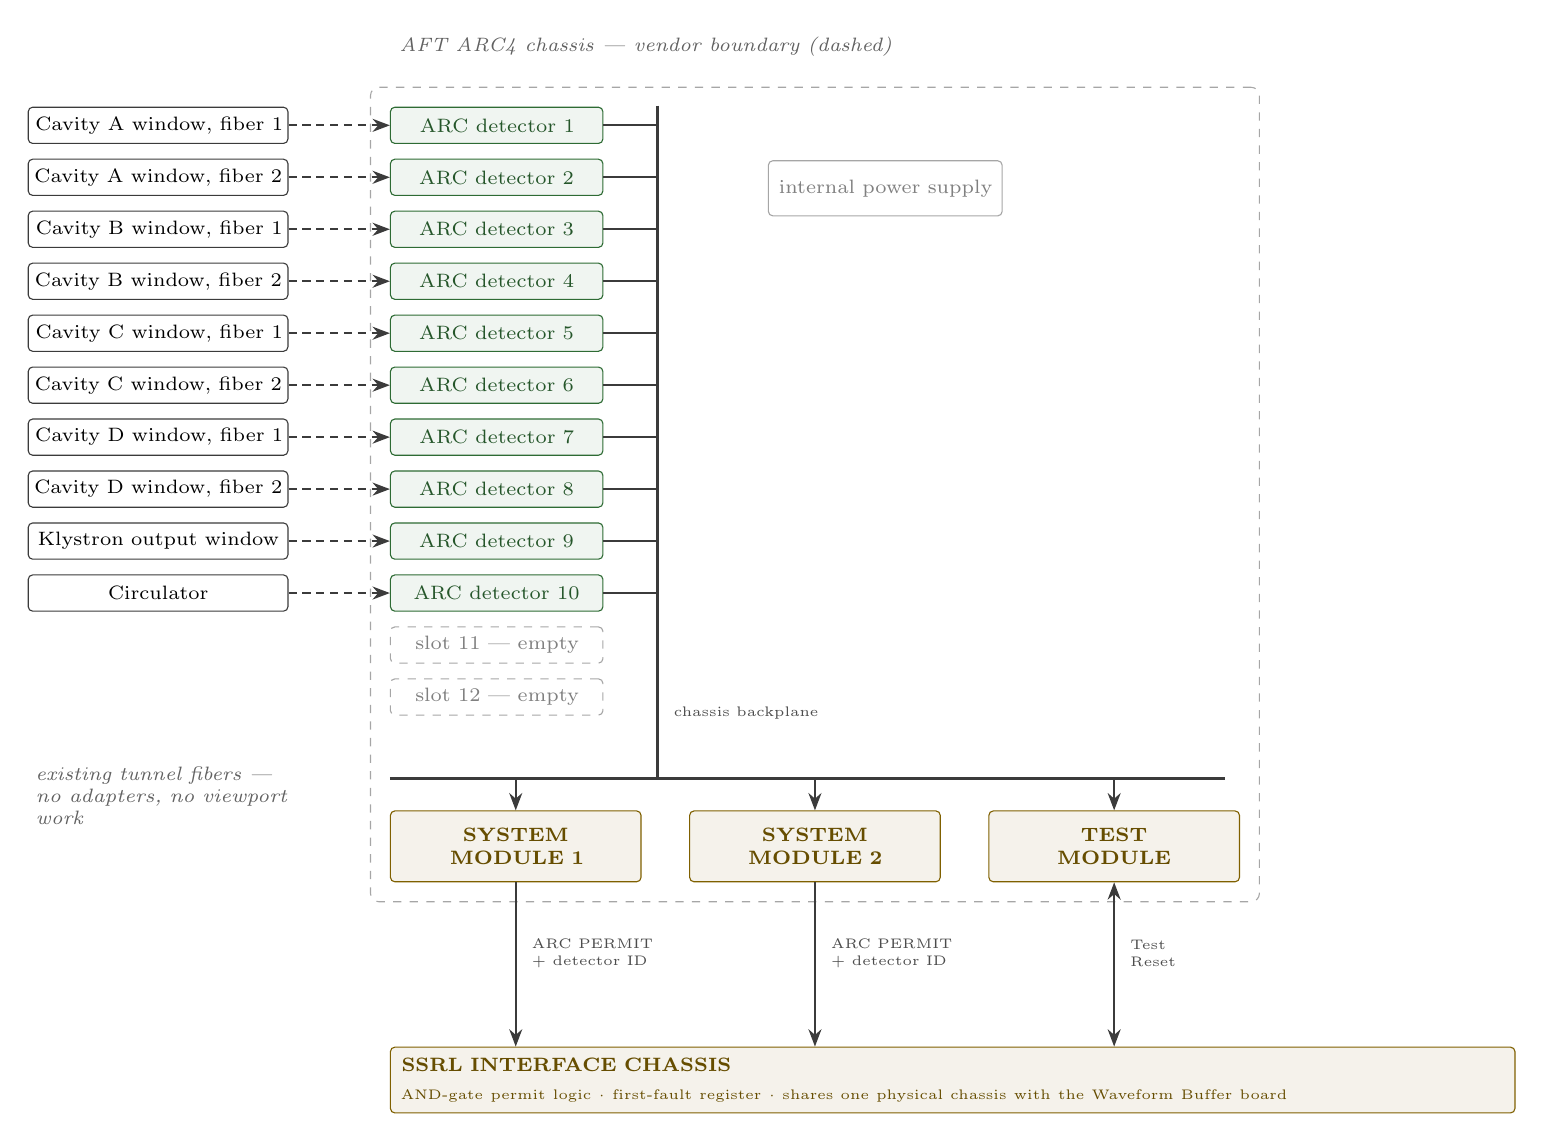
\begin{tikzpicture}[font=\scriptsize, x=1mm, y=1mm,
  src/.style={blk,text width=32mm,minimum height=4.6mm,inner sep=1.4pt,
              font=\scriptsize,anchor=west},
  det/.style={rf,text width=26mm,minimum height=4.6mm,inner sep=1.4pt,
              font=\scriptsize,anchor=west},
  mod/.style={plc,text width=30mm,minimum height=9mm,inner sep=2.6pt,
              align=center,anchor=north west},
  gry/.style={draw=black!35,text=black!50,dashed,fill=white},
]

\def\dy{6.6}
\def\xbus{80}     % vertical backplane collection bus
\def\yrail{-83}   % horizontal backplane rail

% ===== fibers in, one detector module each ==============================
\foreach [count=\i from 0] \s in {%
  {Cavity A window, fiber 1},
  {Cavity A window, fiber 2},
  {Cavity B window, fiber 1},
  {Cavity B window, fiber 2},
  {Cavity C window, fiber 1},
  {Cavity C window, fiber 2},
  {Cavity D window, fiber 1},
  {Cavity D window, fiber 2},
  {Klystron output window},
  {Circulator}}{%
    \pgfmathsetmacro\y{-\i*\dy}
    \pgfmathtruncatemacro\n{\i+1}
    \node[src] (s\i) at (0,\y) {\s};
    \node[det] (d\i) at (46,\y) {ARC detector \n};
    \draw[fib] (s\i.east) -- (d\i.west);
    \draw[draw=cNeut,thick] (d\i.east) -- (\xbus,\y);
  }
% Slots 11 and 12 carry no detector module: the chassis is 12-slot, 10 are
% populated, and the two remaining modules are held as shelf spares.
\foreach [count=\j from 10] \n in {11,12}{%
  \pgfmathsetmacro\y{-\j*\dy}
  \node[det,gry] (d\j) at (46,\y) {slot \n{} --- empty};
}
\node[lbl,anchor=north west,text width=34mm] at (0,-12*\dy-1)
  {existing tunnel fibers ---\\ no adapters, no viewport work};

% ===== chassis backplane ================================================
\draw[bus] (\xbus,2.5) -- (\xbus,\yrail);
\draw[bus] (46,\yrail) -- (152,\yrail);
\node[tag,anchor=south west] at (\xbus+1.5,-76) {chassis backplane};

% ===== internal power supply (no external connection) ===================
\node[blk,text width=28mm,minimum height=7mm,inner sep=2.4pt,anchor=west,
      draw=black!35,text=black!50] at (94,-8)
  {internal power supply};

% ===== system and test modules ==========================================
\node[mod] (sm1) at (46,-87)  {\textbf{SYSTEM}\\\textbf{MODULE 1}};
\node[mod] (sm2) at (84,-87)  {\textbf{SYSTEM}\\\textbf{MODULE 2}};
\node[mod] (tst) at (122,-87) {\textbf{TEST}\\\textbf{MODULE}};
\foreach \m in {sm1,sm2,tst}{\draw[sig] ($(\m.north)+(0,4)$) -- (\m.north);}

% ===== vendor boundary ==================================================
\node[grp,fit=(d0)(d11)(sm1)(tst)] {};
\node[lbl,anchor=west] at (46,10) {AFT ARC4 chassis --- vendor boundary (dashed)};

% ===== SSRL interface chassis ===========================================
\node[plc,text width=140mm,anchor=north west,align=left,inner sep=4pt]
  (ic) at (46,-117)
  {\textbf{SSRL INTERFACE CHASSIS}\\[2pt]
   {\tiny AND-gate permit logic $\cdot$ first-fault register $\cdot$
    shares one physical chassis with the Waveform Buffer board}};

\draw[sig] (sm1.south) -- (sm1.south|-ic.north);
\node[tag,anchor=west,align=left] at ($(sm1.south)+(1.5,-9)$)
  {ARC PERMIT\\ + detector ID};
\draw[sig] (sm2.south) -- (sm2.south|-ic.north);
\node[tag,anchor=west,align=left] at ($(sm2.south)+(1.5,-9)$)
  {ARC PERMIT\\ + detector ID};
\draw[{Stealth[length=2.2mm]}-{Stealth[length=2.2mm]},draw=cNeut,thick]
  (tst.south) -- (tst.south|-ic.north);
\node[tag,anchor=west,align=left] at ($(tst.south)+(1.5,-9)$) {Test\\ Reset};
\end{tikzpicture}

\end{fitpicture}
\caption{Arc detection signal path.  The dashed outline is the vendor boundary: everything inside it is AFT ARC4 hardware, and no SSRL wire lands on an individual detector module.  Fibers enter the detector modules from the front; the detector modules drive the chassis backplane; only the two system modules and the test module face the Interface Chassis.  Ten of the chassis's twelve slots are populated; slots 11 and 12 are left empty and their two detector modules are held as shelf spares.}\label{fig:arc-detection}
\end{figure}

\begin{itemize}
\tightlist
\item
  \textbf{Fast trip path}: a detector module that sees light asserts on the backplane, and the system modules combine all detector states into the arc permit presented to the Interface Chassis. The permit is active-high and the whole path is hardware --- no processor, no encoding step --- so the trip reaches the Interface Chassis AND-gate in the same microsecond class as the LLRF9's own FPGA interlocks.
\item
  \textbf{Diagnostic identification path}: the identity of the detector that fired is held inside the ARC4 and presented to the Interface Chassis alongside the permit. The Interface Chassis includes it in the fault status word that the RF MPS PLC reads, so the first-fault record names the specific window rather than only ``arc''.
\item
  \textbf{Test path}: the test module lets the complete chain --- detector module, backplane, system module, Interface Chassis permit input --- be exercised without a real arc. This is what makes a periodic proof test of the arc interlock possible, which the legacy Fast IC arc inputs never supported.
\end{itemize}

\begin{keynote}
\textbf{Open item --- ARC4 external interface definition.} The exact electrical
form of the system-module and test-module interface is not yet fixed: how many
discrete lines there are, their logic levels, whether the fired-detector
identification arrives as parallel bits or as an encoded word, and how the latch
is reset. These must be taken from the AFT ARC4 documentation and settled
\textbf{before the Interface Chassis PCB is laid out}.\openitem{O6}
\end{keynote}

\subsection{Permit Logic}\label{arc-permit-logic}

\begin{itemize}
\tightlist
\item
  The arc permit from the ARC4 system modules is \textbf{active-high} (permit present = no arc); any arc event drives it low --- consistent with the fail-safe convention throughout the Interface Chassis
\item
  The Interface Chassis removes the RF permit immediately upon any arc event
\item
  The fired-detector identification carried in the Interface Chassis fault status word indicates which channel fired, and is held until reset
\item
  If multiple detectors fire simultaneously, all are reported
\item
  Reset requires an explicit EPICS command via the RF MPS after the fault is acknowledged; the reset acts on both the ARC4 latch and the Interface Chassis first-fault register
\end{itemize}

\subsection{Interfaces}\label{arc-interfaces}

\begin{itemize}
\tightlist
\item
  \textbf{Tunnel fibers → ARC4 detector modules}: one existing optical fiber per channel, landed on the detector module front panel. No adapters, no viewport changes.
\item
  \textbf{ARC4 system modules (×2) → Interface Chassis}: arc permit (fail-safe active-high) plus fired-detector identification. Signal count and logic levels not yet defined --- open item \textbf{O6}.
\item
  \textbf{ARC4 test module ↔ Interface Chassis}: test initiate and test response, plus latch reset.
\item
  \textbf{Interface Chassis → RF MPS PLC}: arc permit state and fired-detector identification included in the Interface Chassis fault status word.
\item
  \textbf{RF MPS / EPICS}: per-channel trip status PVs, fired-detector identification, event count, latch reset command.
\item
  \textbf{EPICS Coordinator}: reads arc fault status for operator displays and state machine fault handling.
\end{itemize}

\textbf{Not an interface}: nothing outside the ARC4 connects to an individual detector module. Adding or moving a channel is a change inside the vendor chassis only, and does not touch the Interface Chassis design.

\begin{center}\rule{0.5\linewidth}{0.5pt}\end{center}

\section{Subsystem 9: Klystron Cathode Heater}\label{subsystem-9-klystron-cathode-heater}

\begin{quote}
\textbf{Detailed reference}: \fpath{llrf/documentation/filamentHeater/sd3403110002.pdf}
\end{quote}

\subsection{Legacy System}\label{legacy-system-2}

The system was originally designed for the PEP-II B-Factory program at SLAC by P. Corredoura and the PEP-II LLRF group, and was subsequently adapted for use in the SPEAR3 storage ring RF system at SSRL. It has been in continuous service for over 25 years.

\textbf{Key Design Characteristics}:

Motor-driven variac providing continuously variable AC voltage

10:1 step-down toroidal isolation transformer (T1)

Solid-state relay (SSR) for on/off switching

Comprehensive monitoring: AC voltmeter, AC ammeter, current transformer (Texmate CT), and elapsed-time meter

Remote control interface via Allen-Bradley (A/B) PLC digital/analog I/O

Front-panel indicators (DS1, DS2 green LEDs) and local metering

\textbf{Power Supply Capabilities}:

\begin{longtable}[]{@{}P{\dimexpr 0.5262\linewidth-1.00\tabcolsep\relax}P{\dimexpr 0.4738\linewidth-1.00\tabcolsep\relax}@{}}
\toprule\noalign{}
Parameter & Legacy \\
\midrule\noalign{}
\endhead
\bottomrule\noalign{}
\endlastfoot
AC Input & 120 VAC, 60 Hz \\
Maximum Power Rating & \textasciitilde1 kW (1000 W) \\
Nominal Operating Power & \textasciitilde500 W (actual sustained operation) \\
Nominal Operating Voltage & 68 V (AC, at transformer input) \\
Nominal Operating Current & 7.3 A \\
Transformer Ratio & 10:1 step-down \\
Secondary Output (Post-Transformer) & \textasciitilde6.8 V RMS at 73 A \\
Maximum Rating & 14.0 V RMS @ 71 A \\
\end{longtable}

\subsection{Upgraded System}\label{upgraded-system}

The \textbf{TDK Lambda programmable AC power supply} is the selected replacement for the motor-driven variac, and the unit is already in hand. It requires an \textbf{external \qty{60}{\hertz} sync circuit}, which is being designed in-house by B.~Morris, so that the heater output stays phase-locked to the site line rather than free-running against it.\openitem{O7}

\textbf{Key advantages over the legacy variac}:

\begin{itemize}
\tightlist
\item
  Analog voltage programming input --- allows the RF MPS to directly ramp output voltage via a DAC signal, replacing the slow motor-driven variac
\item
  Ethernet interface with an ASCII (SCPI-style) command set --- enables EPICS monitoring and enable/disable control via an ASYN driver module
\item
  Solid-state, no mechanical wear
\end{itemize}

\begin{longtable}[]{@{}P{\dimexpr 0.2440\linewidth-1.33\tabcolsep\relax}P{\dimexpr 0.2177\linewidth-1.33\tabcolsep\relax}P{\dimexpr 0.5383\linewidth-1.33\tabcolsep\relax}@{}}
\toprule\noalign{}
\begin{minipage}[b]{\linewidth}\raggedright
Parameter
\end{minipage} & \begin{minipage}[b]{\linewidth}\raggedright
Legacy
\end{minipage} & \begin{minipage}[b]{\linewidth}\raggedright
Upgraded (TDK Lambda)
\end{minipage} \\
\midrule\noalign{}
\endhead
\bottomrule\noalign{}
\endlastfoot
Control method & Motor-driven variac & Programmable AC supply, analog voltage ramp \\
Line synchronization & Inherent (variac on the line) & External \qty{60}{\hertz} sync circuit, in design (B.~Morris) \\
Response time & Seconds--minutes & \textless100 ms \\
Voltage regulation & not specified & From the selected model's data sheet \\
Reliability & Mechanical wear & Solid-state; MTBF from the data sheet \\
EPICS integration & Limited & ASYN module over Ethernet (monitoring + enable/disable) \\
\end{longtable}

\textbf{Control architecture}:

\begin{itemize}
\tightlist
\item
  \textbf{MPS controls the supply} via an analog ramp on the programming input. The RF MPS PLC DAC output drives the TDK Lambda voltage programming pin, setting the output level. This keeps the safety-critical ramp control in hardware (MPS) with fast response.
\item
  \textbf{External \qty{60}{\hertz} sync}: an in-house circuit (B.~Morris) supplies the line-frequency reference to the supply. It is a new design item and is on the heater subsystem's critical path.
\item
  \textbf{EPICS communicates via Ethernet} for monitoring and enable/disable. An ASYN EPICS module will be developed to provide readback PVs (output voltage, current, status) and to send enable/disable commands from the EPICS coordinator.
\item
  \textbf{Existing V/I metering retained}: The current analog voltage and current meters (feeding MPS analog inputs) are kept in place to provide hardware-level monitoring of the output within rating limits, independent of the Ethernet path.
\end{itemize}

\begin{figure}[tbp]
\centering
\begin{fitpicture}% !TeX root = ../0_system_design_report.tex
% Figure 5 -- klystron heater controller architecture.  The control chain runs
% down the left; the two monitoring paths branch to the right.  All row members
% use anchor=west at a common y so the horizontal links are exactly horizontal.
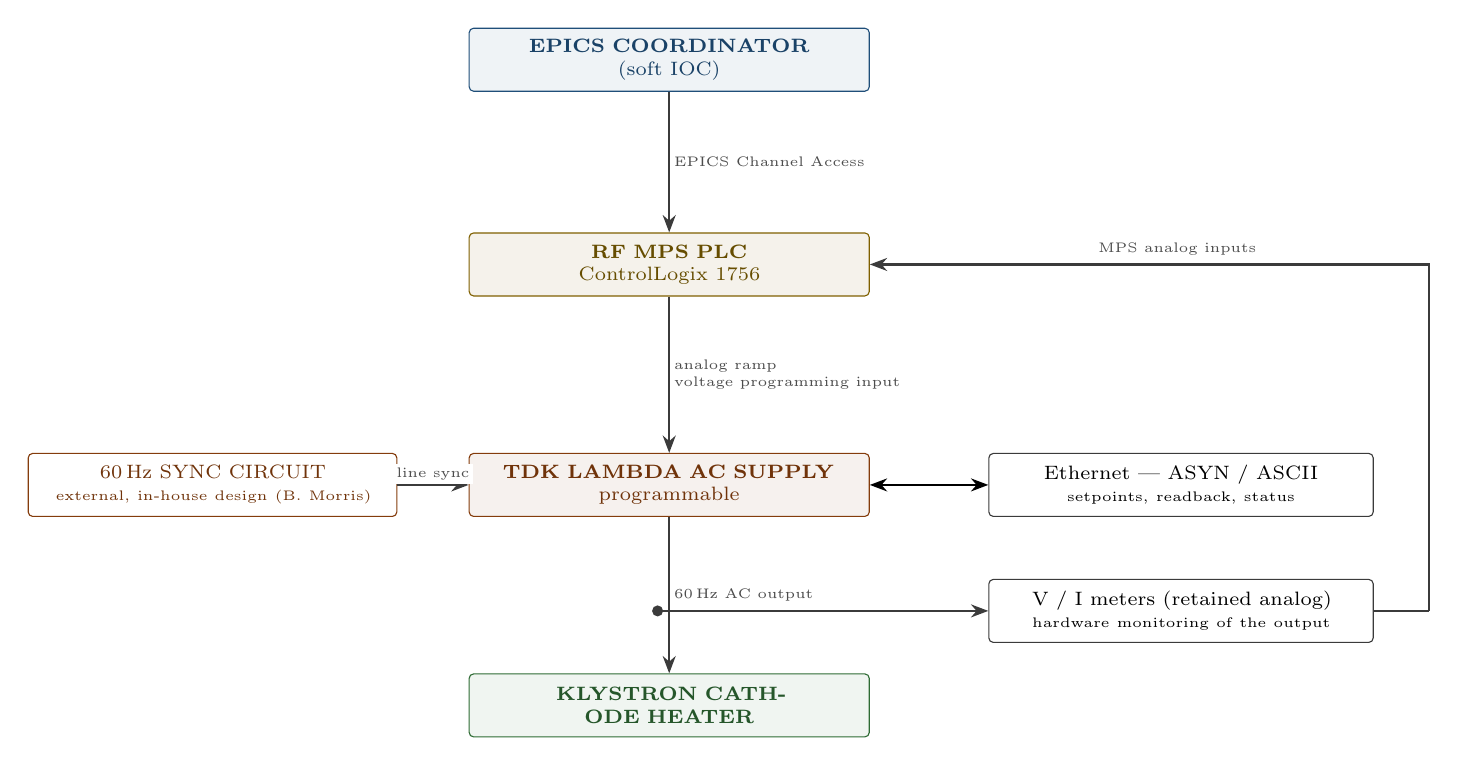
\begin{tikzpicture}[font=\scriptsize, x=1mm, y=1mm]

\node[ctrl,text width=48mm,anchor=west] (ep)  at (10,0)
  {\textbf{EPICS COORDINATOR}\\ (soft IOC)};
\node[plc,text width=48mm,anchor=west]  (mps) at (10,-26)
  {\textbf{RF MPS PLC}\\ ControlLogix 1756};
\node[pwr,text width=48mm,anchor=west]  (ch)  at (10,-54)
  {\textbf{TDK LAMBDA AC SUPPLY}\\ programmable};
\node[rf,text width=48mm,anchor=west]   (kc)  at (10,-82)
  {\textbf{KLYSTRON CATHODE HEATER}};

\draw[sig] (ep.south)  -- node[right,tag]{EPICS Channel Access} (mps.north);
\draw[sig] (mps.south) -- node[right,tag,align=left]
  {analog ramp\\{\tiny voltage programming input}} (ch.north);
\draw[sig] (ch.south)  -- node[right,tag]{\qty{60}{\hertz} AC output} (kc.north);

% --- external line-frequency sync, new in-house design item --------------
\node[blk,text width=44mm,anchor=west,draw=cPwr,text=cPwr!85!black] (sy) at (-46,-54)
  {\qty{60}{\hertz} SYNC CIRCUIT\\{\tiny external, in-house design (B.~Morris)}};
\draw[sig] (sy.east) -- node[above,tag]{line sync} (ch.west);

% --- Ethernet: setpoints and readback, same row as the supply -------------
\node[blk,text width=46mm,anchor=west] (eth) at (76,-54)
  {Ethernet --- ASYN / ASCII\\{\tiny setpoints, readback, status}};
\draw[{Stealth[length=2.2mm]}-{Stealth[length=2.2mm]},thick] (ch.east) -- (eth.west);

% --- retained analog V/I metering, tapped off the supply output -----------
\node[blk,text width=46mm,anchor=west] (vi) at (76,-70)
  {V / I meters (retained analog)\\{\tiny hardware monitoring of the output}};
\fill[cNeut] (34,-70) circle (0.7);
\draw[sig] (34,-70) -- (vi.west);
% return to the MPS analog inputs, routed clear of everything on the far right
\draw[draw=cNeut,thick] (vi.east) -- (132,-70);
\draw[sig] (132,-70) |- (mps.east);
\node[tag,anchor=south] at (100,-25.4) {MPS analog inputs};

\end{tikzpicture}
\end{fitpicture}
\caption{Klystron cathode heater controller architecture.  Three paths are deliberately separate: the MPS ramps the TDK Lambda output through the \emph{analog} programming input, so controlled warm-up and cooldown do not depend on the network; the Ethernet link carries setpoints and readback only; and the existing analog V/I meters are retained, so the delivered output is monitored in hardware independently of both.  The external \qty{60}{\hertz} sync circuit is a new in-house design item.  There are no mechanical components anywhere in the control path.}\label{fig:heater-architecture}
\end{figure}
\textbf{Key design considerations}:

\begin{itemize}
\tightlist
\item
  MPS ramps the supply output voltage via analog programming input for controlled warm-up and cooldown; no mechanical components
\item
  External \qty{60}{\hertz} sync circuit to be designed, built and tested (B.~Morris) before the supply can be commissioned
\item
  ASYN EPICS module required to interface to the TDK Lambda Ethernet port; module to be developed once the model and its command subset are fixed
\item
  Existing analog V/I metering feeds MPS hardware inputs directly --- hardware protection path is independent of Ethernet/EPICS
\item
  Automated warm-up, standby, and cooldown sequences managed by the EPICS coordinator
\item
  Heater interlock: klystron does not receive an RF permit until the heater has reached operating power and the soak timer has elapsed; EPICS provides an expert override for short power dips
\end{itemize}

\subsection{Interfaces}\label{interfaces-3}

\begin{itemize}
\tightlist
\item
  \textbf{RF MPS → TDK Lambda (hardware control)}: MPS PLC DAC output drives the analog voltage programming input. Output is ramped up/down under MPS control for warm-up and cooldown sequences. MPS also provides the hardware enable/disable signal.
\item
  \textbf{Sync circuit → TDK Lambda}: external \qty{60}{\hertz} line-frequency reference, in-house design (B.~Morris).
\item
  \textbf{EPICS → TDK Lambda (monitoring + soft control)}: ASYN EPICS module communicates over Ethernet using an ASCII command set. Provides readback PVs for output voltage, current, and status; sends enable/disable commands from the EPICS coordinator.
\item
  \textbf{Existing V/I metering (retained)}: Legacy analog voltage and current meters feed MPS analog inputs directly, providing hardware-level protection independent of the Ethernet path. Output is monitored against rating limits.
\item
  \textbf{HVPS coordination}: Heater must be at operating temperature before HVPS enable; HVPS must be off before heater cooldown.
\item
  \textbf{RF MPS permit}: Heater ``ready'' status required for RF permit. Hardware heater current and voltage monitored by MPS analog inputs.
\end{itemize}

\begin{center}\rule{0.5\linewidth}{0.5pt}\end{center}

\section{Subsystem 10: Control Software}\label{subsystem-10-control-software}

\begin{quote}
\textbf{Detailed reference}: \fpath{spear-rf-code-legacy/rfApp/src/seq/}, \fpath{Docs_JS/LLRFOperation_jims.docx}
\end{quote}

\subsection{Legacy Software}\label{legacy-software}

The legacy control software consists of SNL (State Notation Language) programs running on VxWorks RTOS in the VXI crate processor:

\begin{longtable}[]{@{}P{\dimexpr 0.2077\linewidth-1.33\tabcolsep\relax}P{\dimexpr 0.0763\linewidth-1.33\tabcolsep\relax}P{\dimexpr 0.7161\linewidth-1.33\tabcolsep\relax}@{}}
\toprule\noalign{}
\begin{minipage}[b]{\linewidth}\raggedright
Program
\end{minipage} & \begin{minipage}[b]{\linewidth}\raggedright
Lines
\end{minipage} & \begin{minipage}[b]{\linewidth}\raggedright
Function
\end{minipage} \\
\midrule\noalign{}
\endhead
\bottomrule\noalign{}
\endlastfoot
\fpath{rf_states.st,v} & 2,227 & Master state machine (OFF/PARK/TUNE/ON\_CW), turn-on, fault handling \\
\fpath{rf_dac_loop.st,v} & 290 & DAC control loop (gap voltage regulation) \\
\fpath{rf_hvps_loop.st,v} & 343 & HVPS control loop (drive power regulation) \\
\fpath{rf_tuner_loop.st,v} & 555 & Tuner control (×4 cavities, phase-based, load angle) \\
\fpath{rf_calib.st,v} & 3,345 & Calibration (analog offset nulling, coefficient calibration, \textasciitilde20 min) \\
\fpath{rf_msgs.st,v} & 352 & Message logging, HVPS faults, TAXI error detection \\
\textbf{Total} & \textbf{7,112} & Six programs, one \texttt{rfSeq} IOC library \\
\end{longtable}

Line counts are the head revision of each RCS archive in \fpath{spear-rf-code-legacy/rfApp/src/seq/}, counted including blank and comment lines.

\subsection{Upgraded Software --- EPICS/MATLAB Coordinator}\label{upgraded-software-epicsmatlab-coordinator}

\begin{quote}
\textbf{Note}: Much of the new software functionality will already be in the LLRF9 internal EPICS IOC (written by Dmitry). Additional supervisory software will be in EPICS/Python/MATLAB as needed.
\end{quote}

The upgrade replaces all SNL code with an EPICS/MATLAB coordinator application that operates as a supervisory control layer at \textasciitilde1 Hz. It is NOT in the fast safety path.

\subsection{Key Design Principles}\label{key-design-principles}

\begin{itemize}
\tightlist
\item
  \textbf{Separation of concerns}: Each module has a single responsibility
\item
  \textbf{Hardware abstraction}: All hardware interfaces go through the EPICS layer
\item
  \textbf{Configuration-driven}: All operational parameters in configuration files
\item
  \textbf{Fault tolerance}: Graceful degradation when subsystems are unavailable
\item
  \textbf{Diagnostics}: Structured event logging, LLRF9 + waveform buffer readout, system performance metrics, and logging
\item
  \textbf{Testability}: Mock interfaces for all hardware dependencies
\item
  \textbf{Safety delegation}: Hardware safety handled by Interface Chassis; software handles sequencing and coordination only
\end{itemize}

\begin{center}\rule{0.5\linewidth}{0.5pt}\end{center}

\section{Control Loop Architecture}\label{control-loop-architecture}

This section maps the control loops in the system, identifying which hardware subsystem closes each loop, the loop bandwidth, and the upgrade path.

\subsection{Fast RF Feedback (Direct Loop)}\label{fast-rf-feedback-direct-loop}

This is the fastest loop in the system and is entirely closed inside the LLRF9 FPGA. The EPICS coordinator does NOT participate.

\subsection{HVPS Supervisory Loop (\textasciitilde1 Hz)}\label{hvps-supervisory-loop-1-hz}

This loop trims the HVPS voltage setpoint to hold the requested operating point while respecting vacuum, gap-voltage and klystron-power limits. \textbf{The supervisory function is unchanged by the upgrade}; only the endpoints it reads and writes change.

The legacy implementation is \fpath{rf_hvps_loop.st,v} (343 lines), which runs a 0.5\,s cycle with a 10\,s hard deadline and operates in one of three states --- \texttt{off}, \texttt{proc} and \texttt{on}:

\begin{itemize}
\tightlist
\item
  \textbf{PROC (cavity processing)}: each cycle the loop compares klystron forward power against its limit and checks the cavity vacuum and gap-voltage alarm severities. If any is bad it applies a fixed negative step to the voltage setpoint; if all are good it applies a fixed positive step. This is what walks the cavities up in voltage during conditioning.
\item
  \textbf{ON (normal operation)}: the correction step is taken from the drive-power error when the direct loop is closed, or from the station gap-voltage error when it is not. The result is clamped to the configured voltage minimum and maximum.
\item
  \textbf{Tolerance supervision}: if the voltage readback disagrees with the requested value by more than the allowed difference for 10 consecutive cycles, the loop holds the setpoint and raises a status code rather than continuing to drive. A separate 10-cycle counter guards the case where the cavities are already at their voltage limit.
\end{itemize}

The loop reports one of 16 status codes (for example \texttt{GOOD}, \texttt{CAVV\_LIM}, \texttt{VOLT\_TOL}, \texttt{VOLT\_LIM}, \texttt{VACM\_BAD}) together with a human-readable string, so the operator sees \emph{why} the loop is holding rather than only that it is.

\textbf{In the upgrade} the same algorithm runs in the EPICS coordinator at \textasciitilde1 Hz. The differences are all at the interfaces: the voltage setpoint and readback move over Ethernet to the CompactLogix HVPS PLC instead of through the Allen-Bradley serial link to the SLC-500, and the gap-voltage and drive-power inputs come from the LLRF9 units rather than from the RFP and IQA modules. Because the Waveform Buffer System now measures HVPS voltage and current directly, the loop also has a true power reading available where the legacy loop had only a forward-power proxy.

\subsection{Tuner Control Loops (×4, \textasciitilde1 Hz)}\label{tuner-control-loops-4-1-hz}

One loop per cavity nulls the cavity detuning by driving the tuner stepper motor until the probe-to-forward phase difference reaches its setpoint. \textbf{The control law is unchanged by the upgrade.}

The legacy implementation is \fpath{rf_tuner_loop.st,v} (555 lines), instantiated four times --- once per cavity --- with five states (\texttt{loop\_init}, \texttt{loop\_unknown}, \texttt{loop\_off}, \texttt{loop\_reset}, \texttt{loop\_on}). Each cycle it:

\begin{enumerate}
\tightlist
\item
  reads the cavity phase error (probe phase minus forward phase);
\item
  converts it to a tuner position delta through the per-cavity gain;
\item
  clamps the resulting position to the motor drive limits and skips the move entirely if the change falls inside the deadband, so the tuner does not chatter;
\item
  commands the move and then waits for the motor's done-moving flag before trusting the new position.
\end{enumerate}

Guards are on the motion rather than the arithmetic: five consecutive failed moves raise a motor-stall status, a missing or bad-severity phase measurement stops motion rather than moving on stale data, and forward power below the configured minimum disables the loop. There is a separate homing sequence with distinct home positions for the ON and PARK states, retried up to five times. The loop reports 14 status codes distinguishing the warning cases (at a drive limit, not at requested position, taking too long to move) from the non-functional cases (bad tuner readback, missing measurements, RF power too low).

\textbf{In the upgrade} the phase measurement comes from the LLRF9 units, which deliver all four cavity probe phases at 10 Hz with sub-degree resolution --- an order of magnitude better than the legacy IQA chain --- and the motor command goes to the Galil DMC-4143 through EPICS motor records instead of to the Allen-Bradley 1746-HSTP1. The LLRF9 also provides its own built-in tuner control PVs (\texttt{GAIN\_P}, \texttt{GAIN\_I}, \texttt{OFFSET}, \texttt{CLOSE}, \texttt{MINFWD} per cavity), so the loop can either be closed inside the LLRF9 or run in the coordinator using LLRF9 phase data. Which of the two is used is a commissioning decision\openitem{O8}; the deadband, drive-limit and stall guards above are required either way.

\subsection{Load Angle Offset Loop (\textasciitilde1 Hz)}\label{load-angle-offset-loop-1-hz}

This outer loop balances gap voltage across the four cavities by biasing the individual tuner phase setpoints, as described in Section~\ref{load-angle-offset-loop}. It reads the four cavity probe amplitudes, computes the imbalance, and adjusts each cavity's phase offset to redistribute power.

\textbf{Legacy status}: the framework exists inside \fpath{rf_tuner_loop.st,v} and the offset is computed in the EPICS database, but it is \emph{not used} on SPEAR3 --- the phase offset fed to the tuner servo is fixed at zero, so the legacy tuners run in pure resonance-seeking mode. The mechanism is inherited from PEP-II, where it regulated cavity voltage in park mode.

\textbf{In the upgrade} the loop becomes a distinct supervisory module in the EPICS coordinator rather than logic buried in the tuner sequencer, writing to the per-cavity tuner phase offset. Whether it is enabled is an operational decision; if it is, it needs an integrator limit and a hold condition tied to tuner loop health, because an outer loop writing into a servo that is itself faulted is a known way to walk a tuner into a limit.

\subsection{Station State Machine}\label{station-state-machine}

The station sequencer owns turn-on, turn-off, mode changes and the response to a fault. \textbf{The sequencing responsibility is unchanged by the upgrade}; the state set is simplified because much of the legacy complexity existed to manage PEP-II loops that SPEAR3 does not use.

The legacy implementation is \fpath{rf_states.st,v} (2,227 lines) --- by a wide margin the largest piece of legacy control software. It comprises 23 states across three concurrent state sets:

\begin{itemize}
\tightlist
\item
  \textbf{5 operating states}: \texttt{OFF}, \texttt{PARK}, \texttt{TUNE}, \texttt{ON\_FM}, \texttt{ON\_CW}.
\item
  \textbf{12 transition substates} that carry the station between them, including the orderly shutdown, the station-reset retry, and the fault-file capture.
\item
  \textbf{5 loop-protection substates} that ramp gap voltage up and down and ramp the direct and comb loop gains, plus a concurrent fault-file writer.
\end{itemize}

Not every transition is legal. \texttt{PARK} cannot go directly to either ON state --- it must pass through \texttt{TUNE} --- and returning from \texttt{ON\_CW} to a lower state is routed through a controlled fallback rather than a direct jump. On a fault the sequencer captures the fault waveform files, performs an orderly shutdown, and then attempts an automatic restart up to a retry limit; a forced-fault latch blocks that automatic restart until an operator clears it.

\textbf{In the upgrade} the sequencer moves to the EPICS coordinator and the state set collapses, because \texttt{ON\_FM} and the comb and gap-voltage-feedback ramps it existed to manage are PEP-II features that SPEAR3 does not use (Section~\ref{eliminated-loops}). Ramping drive power and closing the field loop become LLRF9 operations; the HVPS turn-on and turn-off sequences become CompactLogix operations; tuner homing becomes a Galil operation. What the coordinator retains is exactly the part that was always supervisory: deciding which transitions are legal, ordering the subsystem operations, arming and clearing the fault response, and enforcing the retry limit and the forced-fault latch.

The one behaviour that must be preserved carefully is the interaction with the protection chain. The legacy sequencer could afford to be in the trip path because it ran on a real-time kernel; the upgraded coordinator is explicitly \emph{not} in the fast safety path (Section~\ref{protection-philosophy}), so the state machine must react to a trip that the Interface Chassis has already executed, rather than being the thing that executes it.

\subsection{Calibration}\label{calibration}

Calibration nulls the offsets through the RF signal chain and measures the modulator response so that commanded I/Q corresponds to actual field. \textbf{The need is unchanged by the upgrade; the implementation is entirely replaced.}

The legacy implementation is \fpath{rf_calib.st,v}, 3,345 lines running a 28-state sequence that takes about 20 minutes. Each stage performs a binary search on a DAC channel, settling after each step, averaging a long I/Q record, and halving the step until the residual is within one LSB. It works through the cavity modulator terms, the direct loop, the comb loop, the summing and gain stages, the klystron stage and demodulator, and the final modulator null --- on the order of sixty DAC channels. It aborts cleanly on operator interrupt, on a missing comb module, and when RF is not enabled, restoring the saved DAC values on the way out.

\textbf{In the upgrade} almost all of this disappears with the hardware it calibrated. The offsets being nulled were those of the analog RFP signal chain; the LLRF9 performs its own internal calibration of its ADC and DAC chains and provides it as a built-in function. What remains at the system level is the \emph{station} calibration that no single unit can do for itself: establishing the phase and amplitude relationship between the two LLRF9 units, the cable-length and coupler-calibration constants that convert LLRF9 readings into cavity gap voltage and waveguide power, and the tuner phase reference per cavity. These are coordinator-level procedures operating on LLRF9 measurements rather than DAC-level nulling, and they should be expected to take minutes rather than the legacy twenty.

\subsection{Eliminated Loops}\label{eliminated-loops}

The following legacy loops are eliminated in the upgrade because the LLRF9's digital feedback inherently provides their function (note: comb filter and GVF were used for PEP-II, not SPEAR3):

\begin{itemize}
\tightlist
\item
  \textbf{Ripple rejection loop} --- LLRF9 digital feedback inherently rejects power-line ripple
\item
  \textbf{Comb filter loop (CFM)} --- used for PEP-II multi-bunch stabilization, not applicable to SPEAR3
\item
  \textbf{Gap voltage feedback (GVF)} --- used for PEP-II, not SPEAR3; cavity field stabilization now handled by LLRF9 vector sum feedback
\item
  \textbf{4-way branching (DAC loop)} --- Eliminated; LLRF9 controls all via single vector sum
\end{itemize}

\begin{center}\rule{0.5\linewidth}{0.5pt}\end{center}

\section{Inter-Subsystem Interface Matrix}\label{inter-subsystem-interface-matrix}

This matrix summarizes all physical and logical interfaces between subsystems in the upgraded system.

\begin{longtable}[]{@{}P{\dimexpr 0.0933\linewidth-1.82\tabcolsep\relax}P{\dimexpr 0.0881\linewidth-1.82\tabcolsep\relax}P{\dimexpr 0.0881\linewidth-1.82\tabcolsep\relax}P{\dimexpr 0.0881\linewidth-1.82\tabcolsep\relax}P{\dimexpr 0.0881\linewidth-1.82\tabcolsep\relax}P{\dimexpr 0.1455\linewidth-1.82\tabcolsep\relax}P{\dimexpr 0.0881\linewidth-1.82\tabcolsep\relax}P{\dimexpr 0.0567\linewidth-1.82\tabcolsep\relax}P{\dimexpr 0.0881\linewidth-1.82\tabcolsep\relax}P{\dimexpr 0.0881\linewidth-1.82\tabcolsep\relax}P{\dimexpr 0.0881\linewidth-1.82\tabcolsep\relax}@{}}
\toprule\noalign{}
\begin{minipage}[b]{\linewidth}\raggedright
From ~To
\end{minipage} & \begin{minipage}[b]{\linewidth}\raggedright
LLRF9 \#1
\end{minipage} & \begin{minipage}[b]{\linewidth}\raggedright
LLRF9 \#2
\end{minipage} & \begin{minipage}[b]{\linewidth}\raggedright
HVPS PLC
\end{minipage} & \begin{minipage}[b]{\linewidth}\raggedright
RF MPS PLC
\end{minipage} & \begin{minipage}[b]{\linewidth}\raggedright
Interface Chassis
\end{minipage} & \begin{minipage}[b]{\linewidth}\raggedright
Waveform Buffer
\end{minipage} & \begin{minipage}[b]{\linewidth}\raggedright
Arc Detect
\end{minipage} & \begin{minipage}[b]{\linewidth}\raggedright
Motor Ctrl
\end{minipage} & \begin{minipage}[b]{\linewidth}\raggedright
Heater Ctrl
\end{minipage} & \begin{minipage}[b]{\linewidth}\raggedright
EPICS Coord
\end{minipage} \\
\midrule\noalign{}
\endhead
\bottomrule\noalign{}
\endlastfoot
\textbf{LLRF9 \#1} & --- & Interlock daisy (LEMO) & --- & --- & Status (5V digital) & --- & --- & --- & --- & EPICS (Ethernet) \\
\textbf{LLRF9 \#2} & Interlock daisy (LEMO) & --- & --- & --- & Status (5V digital) & --- & --- & --- & --- & EPICS (Ethernet) \\
\textbf{HVPS PLC} & --- & --- & --- & --- & STATUS (fiber), SCR EN (fiber), CROWBAR (fiber) & --- & --- & --- & --- & EPICS (Ethernet) \\
\textbf{RF MPS PLC} & --- & --- & --- & --- & Summary, Heartbeat, Reset (digital) & --- & --- & --- & --- & EPICS (Ethernet) \\
\textbf{Interface Chassis} & Enable (3.2V) & Enable (3.2V) & SCR EN, CROWBAR (fiber) & Fault status (digital) & --- & --- & --- & --- & --- & --- \\
\textbf{Waveform Buffer} & --- & --- & --- & --- & Comparator trips (digital) & --- & --- & --- & --- & EPICS (Ethernet) \\
\textbf{Arc Detect} & --- & --- & --- & --- & Permit + Latching & --- & --- & --- & --- & --- \\
\textbf{Motor Ctrl} & --- & --- & --- & --- & --- & --- & --- & --- & --- & EPICS (Ethernet) \\
\textbf{Heater Ctrl} & --- & --- & --- & --- & --- & --- & --- & --- & --- & EPICS (Ethernet) \\
\textbf{EPICS Coord} & EPICS (Ethernet) & EPICS (Ethernet) & EPICS (Ethernet) & EPICS (Ethernet) & EPICS & EPICS (Ethernet) & --- & EPICS (Ethernet) & EPICS (Ethernet) & --- \\
\textbf{External (SPEAR MPS, Orbit)} & --- & --- & --- & --- & 24V permits & --- & --- & --- & --- & --- \\
\end{longtable}

\subsection{Interface Signal Types Summary}\label{interface-signal-types-summary}

\begin{longtable}[]{@{}P{\dimexpr 0.20\linewidth-1.6\tabcolsep\relax}P{\dimexpr 0.30\linewidth-1.6\tabcolsep\relax}P{\dimexpr 0.24\linewidth-1.6\tabcolsep\relax}P{\dimexpr 0.26\linewidth-1.6\tabcolsep\relax}@{}}
\toprule\noalign{}
\textbf{Type} & \textbf{Used for} & \textbf{Between} & \textbf{Why this medium} \\
\midrule\noalign{}
\endhead
Fiber optic & SCR ENABLE, CROWBAR, STATUS & Interface Chassis $\leftrightarrow$ HVPS & Full galvanic isolation across a building boundary at high voltage; immune to the ground transients a crowbar event produces \\
Digital, opto-isolated & Permits, heartbeat, reset, fault status & Interface Chassis $\leftrightarrow$ MPS, Waveform Buffer, Arc Detect & Deterministic, no protocol stack; response set by propagation not by scan rate \\
LEMO interlock & Interlock daisy-chain & LLRF9 \#1 $\leftrightarrow$ LLRF9 \#2 & Vendor-native interface; propagates a reflected-power trip between units without going through the Interface Chassis \\
Dry contact / solid-state relay & Arc detection outputs & AFT ARC4 system modules $\rightarrow$ Interface Chassis & Vendor-native chassis output; isolated contact closure needs no supply on the SSRL side \\
Analog & Heater voltage programming; HVPS voltage and current; V/I metering & MPS $\rightarrow$ TDK Lambda; HVPS $\rightarrow$ Waveform Buffer and MPS & Continuous quantity with a hardware path that stays valid if the network is down \\
EPICS Channel Access & Setpoints, readbacks, waveforms, status, commands & EPICS coordinator $\leftrightarrow$ all intelligent devices & Supervisory only; every device on it holds its last safe state if the link drops \\
\bottomrule\noalign{}
\end{longtable}

Two conventions apply across all of them. Every permit is \textbf{active-high}, so a broken cable, a lost supply or a dark fiber removes the permit rather than granting it. And every interlock signal that crosses a chassis boundary is isolated --- by optocoupler, by fiber, or by relay contact --- so that no fault current or ground offset propagates between subsystems.

\subsection{Open Interface Questions}\label{open-interface-questions}

Every unsettled interface detail is carried in the master \hyperref[open-items]{\textbf{Open Items}} table in the front matter (p.~\pageref{open-items}). The interface entries in that table are \textbf{O2} (LLRF9 $\leftrightarrow$ Interface Chassis logic levels), \textbf{O4} (Local Control Chassis disposition), \textbf{O5} (Waveform Buffer spare channels), \textbf{O6} (AFT ARC4 $\rightarrow$ Interface Chassis), \textbf{O7} (heater supply), \textbf{O8} (tuner control split) and \textbf{O9} (network addressing). Each must be closed before the corresponding subsystem can be integrated.

\begin{center}\rule{0.5\linewidth}{0.5pt}\end{center}

\section{Protection Chain and Interlock Architecture}\label{protection-chain-and-interlock-architecture}

\subsection{Protection Philosophy}\label{protection-philosophy}

The upgraded system implements a layered protection architecture:

\begin{itemize}
\tightlist
\item
  \textbf{Layer 1 --- LLRF9 FPGA interlocks} (few μs): RF overvoltage, baseband window comparators, internal housekeeping. These are the fastest protection and act within the LLRF9 itself to disable the DAC output.
\item
  \textbf{Layer 2 --- Interface Chassis hardware} (few μs from input change): Aggregates all permit signals and coordinates system-wide protection. All signals are optocoupler-isolated or fiber-optic. First-fault detection identifies the initiating event.
\item
  \textbf{Layer 3 --- RF MPS PLC} (\textasciitilde ms): Aggregates RF interlock status with external safety systems (SPEAR MPS, orbit interlock). Provides reset signal to Interface Chassis.
\item
  \textbf{Layer 4 --- EPICS Coordinator} (\textasciitilde1 s): Supervisory monitoring, logging, fault analysis, and recovery sequencing. NOT in the fast safety path.
\end{itemize}

\subsection{Fault Propagation Example --- RF Arc Event}\label{fault-propagation-example-rf-arc-event}

\begin{figure}[tbp]
\centering
\begin{fitpicture}% !TeX root = ../0_system_design_report.tex
% Figure 6 -- fault propagation for an RF arc event.  The left column is the
% timescale; each step is roughly three orders of magnitude slower than the one
% above it, which is the whole point of the layered protection scheme.
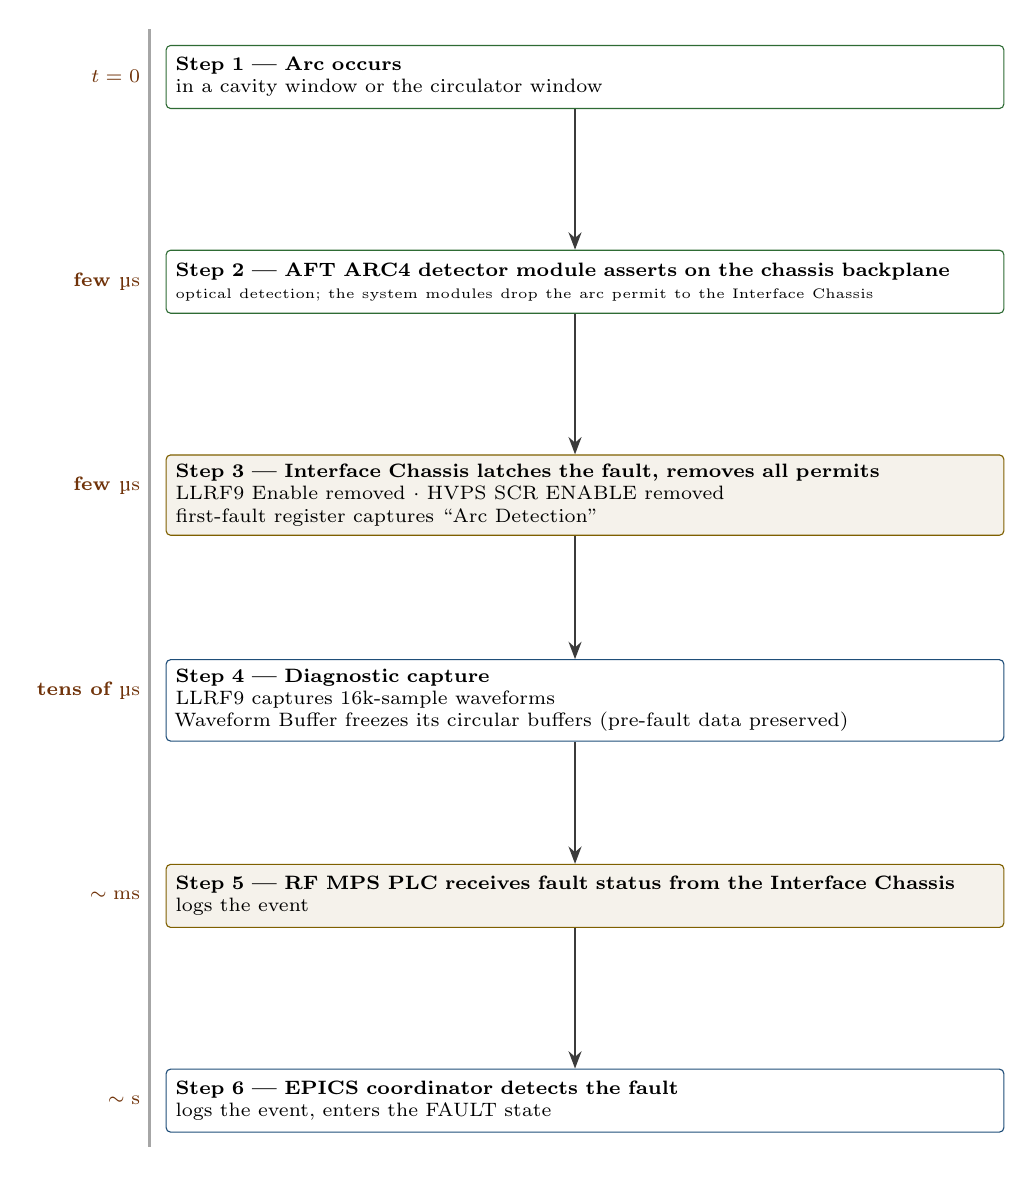
\begin{tikzpicture}[font=\scriptsize, x=1mm, y=1mm,
  stp/.style={blk,text width=104mm,anchor=north west,align=left,inner sep=3.4pt},
  tim/.style={anchor=east,font=\scriptsize\bfseries,text=cPwr!85!black},
]

\def\S{-26}   % step pitch

\node[stp,draw=cRf]   (s1) at (22,0)
  {\textbf{Step 1 --- Arc occurs}\\
   in a cavity window or the circulator window};
\node[tim] at (20,-4) {$t=0$};

\node[stp,draw=cRf]   (s2) at (22,\S)
  {\textbf{Step 2 --- AFT ARC4 detector module asserts on the chassis backplane}\\
   {\tiny optical detection; the system modules drop the arc permit to the Interface Chassis}};
\node[tim] at (20,\S-4) {few \unit{\micro\second}};

\node[stp,draw=cPlc,fill=cPlc!8] (s3) at (22,2*\S)
  {\textbf{Step 3 --- Interface Chassis latches the fault, removes all permits}\\
   LLRF9 Enable removed $\cdot$ HVPS SCR ENABLE removed\\
   first-fault register captures ``Arc Detection''};
\node[tim] at (20,2*\S-4) {few \unit{\micro\second}};

\node[stp,draw=cCtrl] (s4) at (22,3*\S)
  {\textbf{Step 4 --- Diagnostic capture}\\
   LLRF9 captures \num{16}k-sample waveforms\\
   Waveform Buffer freezes its circular buffers (pre-fault data preserved)};
\node[tim] at (20,3*\S-4) {tens of \unit{\micro\second}};

\node[stp,draw=cPlc,fill=cPlc!8] (s5) at (22,4*\S)
  {\textbf{Step 5 --- RF MPS PLC receives fault status from the Interface
   Chassis}\\ logs the event};
\node[tim] at (20,4*\S-4) {$\sim\unit{\milli\second}$};

\node[stp,draw=cCtrl] (s6) at (22,5*\S)
  {\textbf{Step 6 --- EPICS coordinator detects the fault}\\
   logs the event, enters the FAULT state};
\node[tim] at (20,5*\S-4) {$\sim\unit{\second}$};

\foreach \a/\b in {s1/s2,s2/s3,s3/s4,s4/s5,s5/s6}{%
  \draw[sig] (\a.south west) ++(52,0) -- ($(\b.north west)+(52,0)$);}

% timescale rail
\draw[bus,draw=black!35] (20,2) -- (20,5*\S-10);
\end{tikzpicture}
\end{fitpicture}
\caption{Fault propagation for an RF arc event.  Steps 1--3 are pure hardware and complete within a few microseconds: protection is finished before any programmable device is involved.  Each of the remaining steps is roughly three orders of magnitude slower than the one above it, and steps 4--6 are diagnostic and supervisory only --- no protective action depends on them, so a PLC or IOC failure degrades observability but never safety.}\label{fig:fault-propagation}
\end{figure}
\subsection{Fail-Safe Design}\label{fail-safe-design}

All critical subsystems are designed to fail safe:

\begin{longtable}[]{@{}P{\dimexpr 0.2179\linewidth-1.33\tabcolsep\relax}P{\dimexpr 0.2146\linewidth-1.33\tabcolsep\relax}P{\dimexpr 0.5675\linewidth-1.33\tabcolsep\relax}@{}}
\toprule\noalign{}
\begin{minipage}[b]{\linewidth}\raggedright
Subsystem
\end{minipage} & \begin{minipage}[b]{\linewidth}\raggedright
Failure Mode
\end{minipage} & \begin{minipage}[b]{\linewidth}\raggedright
Safe State
\end{minipage} \\
\midrule\noalign{}
\endhead
\bottomrule\noalign{}
\endlastfoot
Interface Chassis power loss & All outputs de-energize & LLRF9 disabled, HVPS SCR disabled (K4/Ross controlled by separate PPS interface box) \\
LLRF9 power loss & Interlock status goes low & Interface Chassis removes permits \\
HVPS PLC failure & STATUS signal lost & Interface Chassis removes permits \\
RF MPS PLC failure & Heartbeat lost & Interface Chassis removes permits \\
EPICS coordinator crash & No effect on safety & Hardware protection continues; supervisory control paused \\
Ethernet failure & No effect on safety & Hardware protection continues; supervisory control paused \\
\end{longtable}

\begin{center}\rule{0.5\linewidth}{0.5pt}\end{center}

\section{Communication Architecture}\label{communication-architecture}

\subsection{EPICS Channel Access Network}\label{epics-channel-access-network}

All supervisory communication in the upgraded system uses EPICS Channel Access over Ethernet:

\begin{longtable}[]{@{}P{\dimexpr 0.2560\linewidth-1.60\tabcolsep\relax}P{\dimexpr 0.0930\linewidth-1.60\tabcolsep\relax}P{\dimexpr 0.3345\linewidth-1.60\tabcolsep\relax}P{\dimexpr 0.1580\linewidth-1.60\tabcolsep\relax}P{\dimexpr 0.1585\linewidth-1.60\tabcolsep\relax}@{}}
\toprule\noalign{}
\begin{minipage}[b]{\linewidth}\raggedright
Device
\end{minipage} & \begin{minipage}[b]{\linewidth}\raggedright
IP Address
\end{minipage} & \begin{minipage}[b]{\linewidth}\raggedright
IOC Type
\end{minipage} & \begin{minipage}[b]{\linewidth}\raggedright
Key PV Prefix
\end{minipage} & \begin{minipage}[b]{\linewidth}\raggedright
Update Rate
\end{minipage} \\
\midrule\noalign{}
\endhead
\bottomrule\noalign{}
\endlastfoot
LLRF9 Unit 1 & TBD\openitem{O9} & Built-in Linux IOC & \texttt{LLRF1:} & 10 Hz (scalars) \\
LLRF9 Unit 2 & TBD & Built-in Linux IOC & \texttt{LLRF2:} & 10 Hz (scalars) \\
HVPS CompactLogix & TBD & External EPICS gateway & \texttt{SRF1:HVPS:} & \textasciitilde1 Hz \\
RF MPS ControlLogix & TBD & External EPICS gateway & \texttt{SRF1:MPS:} & \textasciitilde1 Hz \\
Motion Controller & TBD & EPICS motor record IOC & \texttt{SRF1:MTR:} & On demand \\
Waveform Buffer & TBD & Dedicated IOC & \texttt{SRF1:WFBUF:} & \textasciitilde1 Hz / event \\
EPICS/MATLAB Coordinator & TBD & caproto / PyEPICS / MATLAB client & Various & \textasciitilde1 Hz \\
\end{longtable}

\subsection{Non-EPICS Communication Paths}\label{non-epics-communication-paths}

\begin{longtable}[]{@{}P{\dimexpr 0.2866\linewidth-1.33\tabcolsep\relax}P{\dimexpr 0.3408\linewidth-1.33\tabcolsep\relax}P{\dimexpr 0.3726\linewidth-1.33\tabcolsep\relax}@{}}
\toprule\noalign{}
\begin{minipage}[b]{\linewidth}\raggedright
Path
\end{minipage} & \begin{minipage}[b]{\linewidth}\raggedright
Type
\end{minipage} & \begin{minipage}[b]{\linewidth}\raggedright
Purpose
\end{minipage} \\
\midrule\noalign{}
\endhead
\bottomrule\noalign{}
\endlastfoot
Interface Chassis ↔ all hardware & Hardwired digital/fiber & Safety interlocks (no network dependency) \\
LLRF9 Unit 1 ↔ Unit 2 & LEMO interlock daisy-chain & Fast interlock propagation \\
PPS ↔ PPS Interface Box & Hardwired (GOB1208PNE) & Personnel safety (no network dependency) \\
AFT ARC4 system modules → Interface Chassis & Dry contact relay and/or semiconductor switches & Arc interlock (no network dependency) \\
\end{longtable}

\textbf{Critical design principle}: All safety-critical communication paths are hardwired. No safety function depends on the Ethernet network or EPICS Channel Access. Network loss pauses supervisory control but does not compromise protection.

\begin{center}\rule{0.5\linewidth}{0.5pt}\end{center}

\section{Implementation Phases and Risk Summary}\label{implementation-phases-and-risk-summary}

\subsection{Implementation Phases}\label{implementation-phases}

\begin{quote}
\textbf{Critical Constraint}: The SPEAR3 LLRF upgrade has extremely limited flexibility for integration testing since bringing systems online directly impacts SPEAR operations. This severely constrains the available testing window and requires a fundamentally different approach than typical development projects.
\end{quote}

\textbf{Key Implications}:

\begin{itemize}
\tightlist
\item
  Maximum standalone subsystem testing must occur before installation
\item
  Integration testing must be incremental and carefully planned
\item
  Some subsystems can be brought online for limited testing without full operational impact
\item
  Full system integration testing window is minimal
\end{itemize}

\subsubsection{Phase 1: Maximum Standalone Development}\label{phase-1-maximum-standalone-development}

\begin{itemize}
\tightlist
\item
  \textbf{Software Framework}: Develop with simulated interfaces where live hardware unavailable
\item
  \textbf{Tuner Testing}: Test Galil controller with Booster RF cavity
\item
  \textbf{LLRF9 Installation}: Install both units, connect RF signals, and bring them online
\item
  \textbf{RF MPS Online}: Bring RF MPS online for EPICS interface development
\item
  \textbf{HVPS PLC Online}: Enables EPICS software development
\item
  \textbf{Waveform Buffer Assembly}: Complete assembly and standalone testing --- \textbf{done, April 2026}
\item
  \textbf{Interface Chassis Design/Fab}: Complete design and fabrication (shares the Waveform Buffer chassis; PCB at fab since August 2026, bench test October 2026)
\item
  \textbf{HVPS Controller}: Design, fabrication, and installation
\item
  \textbf{Arc Detector}: Receive and bench-test the AFT ARC4 chassis and its 12 detector modules; define the system-module interface from vendor documentation. \emph{No SSRL design or fabrication --- this is procurement and integration.}
\item
  \textbf{PPS Interface Box}: Design, fabrication, and commissioning
\item
  \textbf{Test Stand 18}: Upgrade to work with the upgraded HVPS controller
\end{itemize}

\subsubsection{Phase 2: Incremental Subsystem Integration}\label{phase-2-incremental-subsystem-integration}

\begin{itemize}
\tightlist
\item
  \textbf{Tuner Test with SPEAR Cavity}
\item
  \textbf{HVPS Integration}: Integrate HVPS PLC with EPICS coordinator (test at test stand T18)
\item
  \textbf{RF MPS Integration}: Integrate RF MPS with LLRF9, waveform buffer, arc detector, HVPS PLC, interface chassis, and software coordinator with existing RF signals
\end{itemize}

\subsubsection{Phase 3: Critical Path Integration}\label{phase-3-critical-path-integration}

\begin{itemize}
\tightlist
\item
  \textbf{LLRF9 Integration --- Basic RF Processing}: Verify vector sum, feedback loops, online calibration
\item
  \textbf{EPICS Integration}: Configure IOC, verify all PV interfaces
\item
  \textbf{End-to-End Interlock Testing}: Verify complete interlock chain (limited RF power)
\end{itemize}

\subsubsection{Phase 4: Full Power Commissioning}\label{phase-4-full-power-commissioning}

\begin{itemize}
\tightlist
\item
  \textbf{Incremental Power Ramp}: Gradually increase power while monitoring all systems
\item
  \textbf{Performance Validation}: Verify all success criteria are met
\item
  \textbf{Operator Training}: Train operators on new system
\item
  \textbf{Documentation}: Complete commissioning report
\end{itemize}

\subsection{Status}\label{status}

\begin{longtable}[]{@{}P{\dimexpr 0.3966\linewidth-1.33\tabcolsep\relax}P{\dimexpr 0.2683\linewidth-1.33\tabcolsep\relax}P{\dimexpr 0.3351\linewidth-1.33\tabcolsep\relax}@{}}
\toprule\noalign{}
\begin{minipage}[b]{\linewidth}\raggedright
Item
\end{minipage} & \begin{minipage}[b]{\linewidth}\raggedright
Status
\end{minipage} & \begin{minipage}[b]{\linewidth}\raggedright
Notes
\end{minipage} \\
\midrule\noalign{}
\endhead
\bottomrule\noalign{}
\endlastfoot
LLRF9 (4 units) & Hardware complete & Two units installed in B132; RF signals to be hooked up October 2026. Two spares on the shelf. \\
RF MPS PLC modules & Hardware complete & EPICS software under development \\
HVPS PLC modules & Hardware complete (HVPS1, HVPS2, B44 Test Stand) & EPICS software under development \\
Enerpro FCOG1200 boards & On order & 5 boards ordered; awaiting delivery \\
Arc detection (AFT ARC4) & Done & Chassis fully assembled with all modules, September 2026 \\
Waveform Buffer System & \textbf{Complete} & April 2026; shares one chassis with the Interface Chassis \\
Interface Chassis & In progress & Prototype built. Front and back panels to be modified and the chassis raised from 2U to \textbf{3U} to arrange components better; bench test Oct--Nov 2026. \\
Heater Controller (TDK Lambda programmable AC supply) & Supply in hand & Awaiting the software specification; external \qty{60}{\hertz} sync circuit in design (B.~Morris) \\
PPS Interface Box & Initial design done & Awaiting design review \\
Software & In progress & Legacy code review complete; functional requirements being drafted; beta expected Spring 2027 \\
\end{longtable}

\subsection{Key Technical Risks}\label{key-technical-risks}

\begin{longtable}[]{@{}P{\dimexpr 0.2177\linewidth-1.50\tabcolsep\relax}P{\dimexpr 0.0882\linewidth-1.50\tabcolsep\relax}P{\dimexpr 0.0978\linewidth-1.50\tabcolsep\relax}P{\dimexpr 0.5963\linewidth-1.50\tabcolsep\relax}@{}}
\toprule\noalign{}
\begin{minipage}[b]{\linewidth}\raggedright
Risk
\end{minipage} & \begin{minipage}[b]{\linewidth}\raggedright
Severity
\end{minipage} & \begin{minipage}[b]{\linewidth}\raggedright
Status
\end{minipage} & \begin{minipage}[b]{\linewidth}\raggedright
Mitigation
\end{minipage} \\
\midrule\noalign{}
\endhead
\bottomrule\noalign{}
\endlastfoot
Tuner motor controller reliability & High & \textbf{Closed} & Galil tested on SPEAR in August 2026, driving all four cavity tuner motors simultaneously \\
HVPS PLC code migration (SLC-500 → CompactLogix) & High & In progress & Reverse-engineer legacy code; build Test Stand 18 (B44) \\
PPS Interface approval delays & High & In progress & Engage protection managers early; provide complete documentation. Initial design done, awaiting review. \\
Interface Chassis logic design (LLRF9/HVPS feedback loop) & High & In progress & Design and simulate before fabrication; careful sequencing logic. Prototype built; panels being reworked and the chassis raised to 3U; bench test Oct--Nov 2026. \\
Waveform Buffer System (new custom hardware) & Medium & \textbf{Closed} & Staged development completed; board complete April 2026 \\
EPICS/MATLAB Coordinator software & Critical & In progress & Largest software scope: state machine, fault handling, auto-recovery sequences, operator interface, and integration with all subsystem IOCs. Legacy code review complete and functional requirements being drafted; beta expected Spring 2027. Must be developed in parallel with hardware integration. \\
RF MPS PLC software integration & High & In progress & MPS hardware is assembled and tested standalone; EPICS IOC development is under way, but integration with Interface Chassis fault status, first-fault logic and reset sequencing has not begun. \\
AFT ARC4 external interface definition & Medium & In progress & No longer an SSRL firmware task --- the OR and latch functions are inside the vendor chassis. The residual risk is that the system-module and test-module interface must be pinned down from AFT documentation before the Interface Chassis PCB is laid out. \\
Heater supply \qty{60}{\hertz} sync circuit & Medium & In progress & TDK Lambda supply is in hand; the sync circuit design, build and test (B.~Morris) is a new in-house item on the heater critical path, and the software specification is still outstanding. \\
Communication latency (Ethernet/EPICS for \textasciitilde1 Hz control) & Low & Validated & Proven in LLRF9 prototype commissioning \\
\end{longtable}

\subsection{Success Criteria}\label{success-criteria}

\begin{longtable}[]{@{}P{\dimexpr 0.2627\linewidth-1.33\tabcolsep\relax}P{\dimexpr 0.2690\linewidth-1.33\tabcolsep\relax}P{\dimexpr 0.4683\linewidth-1.33\tabcolsep\relax}@{}}
\toprule\noalign{}
\begin{minipage}[b]{\linewidth}\raggedright
Metric
\end{minipage} & \begin{minipage}[b]{\linewidth}\raggedright
Legacy Performance
\end{minipage} & \begin{minipage}[b]{\linewidth}\raggedright
Target
\end{minipage} \\
\midrule\noalign{}
\endhead
\bottomrule\noalign{}
\endlastfoot
Amplitude stability & \textless0.1\% & Same or better \\
Phase stability & \textless0.1 deg & Same or better \\
Tuner resolution & \textasciitilde0.002--0.003 mm/microstep & Improved (up to 256 microsteps/step) \\
Control loop response & \textasciitilde1 second & Same or better \\
Uptime & \textgreater99\% (nominal, not formally measured) & Same or better \\
Fault diagnostics & Limited fault file capture & 16k-sample waveform + circular buffer + first-fault \\
\end{longtable}

\begin{center}\rule{0.5\linewidth}{0.5pt}\end{center}

\section{Appendix: Source Document Index}\label{appendix-source-document-index}

\begin{quote}
Every path below has been checked to exist. Note that the legacy SNL source is RCS-archived under \fpath{spear-rf-code-legacy/rfApp/src/seq/}, so each file carries a \texttt{.st,v} extension --- there is no \fpath{llrf/legacyLLRF/} directory.
\end{quote}

\subsection{Governing project document}\label{governing-project-document}

\begin{longtable}[]{@{}P{\dimexpr 0.4194\linewidth-1.00\tabcolsep\relax}P{\dimexpr 0.5806\linewidth-1.00\tabcolsep\relax}@{}}
\toprule\noalign{}
\begin{minipage}[b]{\linewidth}\raggedright
Path
\end{minipage} & \begin{minipage}[b]{\linewidth}\raggedright
Content
\end{minipage} \\
\midrule\noalign{}
\endhead
\bottomrule\noalign{}
\endlastfoot
\fpath{Designs/docx/SPEAR3\_LLRF\_PDR\_R2.docx} & \textbf{SPEAR3 LLRF Upgrade Preliminary Design Review, R2 (28 April 2026)} --- the authoritative upgrade specification. Sections 1--19 of this report track it directly \\
\fpath{Designs/docx/SPEAR3\_LLRF\_Upgrade\_Project\_Schedule.xlsx} & Project schedule \\
\end{longtable}

\subsection{LLRF Source Material}\label{llrf-source-material}

\begin{longtable}[]{@{}P{\dimexpr 0.6116\linewidth-1.00\tabcolsep\relax}P{\dimexpr 0.3884\linewidth-1.00\tabcolsep\relax}@{}}
\toprule\noalign{}
\begin{minipage}[b]{\linewidth}\raggedright
Path
\end{minipage} & \begin{minipage}[b]{\linewidth}\raggedright
Content
\end{minipage} \\
\midrule\noalign{}
\endhead
\bottomrule\noalign{}
\endlastfoot
\fpath{../spear-rf-code-legacy/rfApp/src/seq/rf_states.st,v} & Legacy master state machine (23 states) \\
\fpath{../spear-rf-code-legacy/rfApp/src/seq/rf_dac_loop.st,v} & Legacy DAC control loop \\
\fpath{../spear-rf-code-legacy/rfApp/src/seq/rf_hvps_loop.st,v} & Legacy HVPS control loop \\
\fpath{../spear-rf-code-legacy/rfApp/src/seq/rf_tuner_loop.st,v} & Legacy tuner control loop \\
\fpath{../spear-rf-code-legacy/rfApp/src/seq/rf_calib.st,v} & Legacy calibration system \\
\fpath{../spear-rf-code-legacy/rfApp/src/seq/rf_msgs.st,v} & Legacy message logging \\
\fpath{../spear-rf-code-legacy/codeReviewTechnicalNotes/} & Nine-part code review of the legacy application \\
\fpath{llrf/architecture/llrfInterfaceChassis.docx} & Interface Chassis specification \\
\fpath{llrf/architecture/WaveformBuffersforLLRFUpgrade.docx} & Waveform Buffer System design \\
\fpath{llrf/architecture/arcDetectorHardwareOptions.docx} & Arc detection hardware selection \\
\fpath{llrf/architecture/rfPowerDetector.docx} & RF power detector selection \\
\fpath{llrf/architecture/analogDesignComponents.docx} & Analog component selection \\
\fpath{llrf/documentation/LLRFOperation\_jims.docx} & SPEAR3 RF Station Operation Guide (J. Sebek) \\
\fpath{llrf/documentation/LLRFUpgradeTaskListRev3.docx} & Full project scope, procurement, costs \\
\fpath{llrf/documentation/fiberOpticCableSignalControlRev3.docx} & Fibre-optic signal and control routing \\
\fpath{../llrf/tuners/galil/} & Galil DMC-4143 firmware and \textbf{test-move logs} (the controller is \emph{not} installed --- see §10) \\
\fpath{../llrf/driveAmp/} & Drive amplifier datasheet (KAW2051M12) \\
\fpath{../llrf/arcDetector/} & Arc detector product sheets and mechanical references \\
\fpath{llrf/tests/llrf9Tests.tex} & LLRF9 commissioning measurements (J. Sebek, 2021) \\
\end{longtable}

\subsection{HVPS Source Material}\label{hvps-source-material}

\begin{longtable}[]{@{}P{\dimexpr 0.5366\linewidth-1.00\tabcolsep\relax}P{\dimexpr 0.4634\linewidth-1.00\tabcolsep\relax}@{}}
\toprule\noalign{}
\begin{minipage}[b]{\linewidth}\raggedright
Path
\end{minipage} & \begin{minipage}[b]{\linewidth}\raggedright
Content
\end{minipage} \\
\midrule\noalign{}
\endhead
\bottomrule\noalign{}
\endlastfoot
\fpath{hvps/documentation/wiringDiagrams/ei7307900000.pdf} & \textbf{EI-730-790-00-C0 / NWL \#39308} --- the transformer manufacturer's own schematic. Authoritative for the \textbf{2750 kVA / 127 A} nameplate and all oil, pressure, vacuum and flow protection setpoints \\
\fpath{hvps/documentation/schematics/sd7307900101.pdf} & SD-730-790-01-C1 --- HVPS system schematic \\
\fpath{hvps/documentation/wiringDiagrams/wd7307940400.pdf} & WD-730-794-04-C0 --- contains the \textbf{HVPS output voltage dividers} \\
\fpath{hvps/documentation/wiringDiagrams/wd7307900206.pdf} & WD-730-790-02-C6 --- master trigger enclosure wiring diagram \\
\fpath{hvps/documentation/procedures/spear3HvpsHazards.tex} & J. Sebek --- stored energy, discharge time constants, klystron perveance \\
\fpath{hvps/architecture/designNotes/EnerproVoltageandCurrentRegulatorBoardNotes.docx} & J. Sebek --- authoritative regulator board circuit analysis \\
\fpath{hvps/architecture/designNotes/RFSystemMPSRequirements.docx} & RF system MPS requirements \\
\fpath{hvps/architecture/originalDocuments/slac-pub-7591.pdf} & Cassel \& Nguyen, PAC 1997 --- crowbar timing, regulation, ripple \\
\fpath{hvps/architecture/originalDocuments/ps3413600102.pdf} & PS-341-360-01 --- HVPS power section specification \\
\fpath{hvps/controls/enerpro/enerproBoardHvps.docx} & J. Sebek --- installed Enerpro board revisions, serials, phase references \\
\fpath{hvps/documentation/plc/CasselPLCCode.pdf} & Full SLC-500 ladder logic listing, program SSRLV6-4-05-10 \\
\fpath{hvps/documentation/plc/plcNotesR1.docx} & J. Sebek --- PLC timing and the N7:10 setpoint filter \\
\fpath{../hvps/documentation/procedures/} & Maintenance and safety procedures, EWPs, lockout permits \\
\fpath{../hvps/maintenance/} & Stack installation checklists, phase tank maintenance \\
\end{longtable}

\subsection{Switchgear and PPS Source Material}\label{switchgear-and-pps-source-material}

\begin{longtable}[]{@{}P{\dimexpr 0.5411\linewidth-1.00\tabcolsep\relax}P{\dimexpr 0.4589\linewidth-1.00\tabcolsep\relax}@{}}
\toprule\noalign{}
\begin{minipage}[b]{\linewidth}\raggedright
Path
\end{minipage} & \begin{minipage}[b]{\linewidth}\raggedright
Content
\end{minipage} \\
\midrule\noalign{}
\endhead
\bottomrule\noalign{}
\endlastfoot
\fpath{hvps/documentation/switchgear/gp3085000103.pdf} & \textbf{GP-308-500-01-R3} (LBL, 1977) --- original design drawing; authoritative \textbf{relay legend}; blocking relay blocks trip above 2000 A \\
\fpath{hvps/documentation/switchgear/gp4397040201.pdf} & GP-439-704-02-C1 --- as-built schematic and sequence of operation \\
\fpath{hvps/documentation/switchgear/id3088010601.pdf} & ID-308-801-06-C1 --- as-built connection wiring \\
\fpath{hvps/documentation/switchgear/rossEngr713203.pdf} & Ross 713203 E-1 --- HCA-1-A driver and HQ3 contactor \\
\fpath{pps/HoffmanBoxPPSWiring.docx} & J. Sebek --- terminal-by-terminal PPS wiring trace \\
\fpath{pps/MSG from Jim Sebek to Faya about PPS.md} & 2022 PPS concerns and upgrade drivers \\
\fpath{pps/diagrams/README.md} & PPS diagram note set and the PPS readback trace \\
\end{longtable}

\begin{comment}
  


\subsection{Companion design documents}\label{companion-design-documents}

\begin{longtable}[]{@{}P{\dimexpr 0.5211\linewidth-1.00\tabcolsep\relax}P{\dimexpr 0.4789\linewidth-1.00\tabcolsep\relax}@{}}
\toprule\noalign{}
\begin{minipage}[b]{\linewidth}\raggedright
Document
\end{minipage} & \begin{minipage}[b]{\linewidth}\raggedright
Content
\end{minipage} \\
\midrule\noalign{}
\endhead
\bottomrule\noalign{}
\endlastfoot
\fpath{Designs/tex/docL-legacy-architecture/L\_legacy\_system\_architecture.pdf} & \textbf{The legacy system reference.} All legacy values in this report should agree with it \\
\fpath{Designs/tex/docI-interlock-architecture/I\_interlock\_architecture.pdf} & Legacy interlock and protection architecture \\
\fpath{Designs/tex/docP-rf-physics/P\_rf\_physics\_and\_plant.pdf} & RF physics, cavity parameters, beam loading \\
\fpath{Designs/tex/docT-tuner-control/T\_tuner\_control\_analysis.pdf} & Tuner control system analysis \\
\end{longtable}

\end{comment}

\begin{center}\rule{0.5\linewidth}{0.5pt}\end{center}



\end{document}
